
\documentclass[11pt,oneside,final]{huthesis}

\usepackage{epsfig,bm,epsf,float}
\usepackage{hyperref}
\usepackage{lscape}
\usepackage[utf8]{inputenc}
\usepackage[authoryear,round,comma]{natbib}
\usepackage[spanish,es-nodecimaldot]{babel}
\usepackage[papersize={170mm,225mm},bmargin=20mm,lmargin=25mm,rmargin=20mm]{geometry}  
\usepackage[ruled,vlined,noend,linesnumbered,spanish]{algorithm2e}
\usepackage{amssymb}
\usepackage{amsmath}
\usepackage{dsfont}
\usepackage{caption}
\usepackage{titlesec}

\def\Var{{\rm{Var}}}
\def\E{{\rm{E}}}
\def\VarN{{\rm{Var_N}}}
\def\EN{{\rm{E_N}}}
\def\VarR{{\rm{Var_R}}}
\def\ER{{\rm{E_R}}}

% \titleformat*{\section}{\LARGE\bfseries}
\titleformat*{\section}{\Large\bfseries}
\titleformat*{\subsection}{\large\bfseries}
\titleformat*{\subsubsection}{\normalsize\bfseries}
\titleformat*{\paragraph}{\normalsize\bfseries}
\titleformat*{\subparagraph}{\normalsize\bfseries}
%\includeonly{\files} 


% Table of contents max depth listed:
% 1 = section, 2 = subsection, 3 = subsubsection
\setcounter{tocdepth}{3}


\begin{document}

% Single spacing
% \ssp
\dsp

%% frontmatter.tex
%%
\title{Análisis de Conglomerados Esférico para Comprobar Autocorrelación Espacial Positiva: Una Aplicación al Índice de Marginación en México}
\author{Carlos Espino García}
\degreemonth{Febrero}
\degreeyear{2015}
\degree{Licenciado en Matemáticas Aplicadas}
\field{Matemáticas Aplicadas}
\department{Matemáticas y Estadística}
\advisor{Dr. Juan José Fernández Durán } 
\place{México, D.F.}

\maketitle
% \maketitle
% \copyrightpage
\makeitamdoc




%We show how a systematic subtraction of the `special' components of a general
%deformation can be used to give an improved
%version of the `wall formula' estimate for $\mu(0)$.
%We believe this is the first study of $\omega$-dependent heating rate in
%billards, and the first consideration of the `special' nature of dilation.





% these are optional in the Jan 2000 Harvard thesis GSAS guide:
%\listoffigures
%\listoftables
%(Cut them for my personal thesis format).

% cccccccccccccccccccccccccccccccccccccccccccccccccccccccccccccccccccccccccc
% \begin{citations}

% \vspace{0.8in}

% \ssp
% \noindent
% % Large portions of Chapters~\ref{ch:dil} and \ref{ch:wall}, as well as some
% % of Sections~\ref{sec:qcc} and \ref{sec:quasi}
% have appeared in the following two papers:
% \begin{quote}
% 	``Deformations and dilations of chaotic billiards:
% 	dissipation rate, and quasi-orthogonality of the boundary
% 	wavefunctions'',
% 	A. H. Barnett, D. Cohen, and E. J. Heller,
% 	Phys. Rev. Lett. {\bf 85}, 1412 (2000), {\tt nlin.CD/0003018};
% 	\vspace{.1in} \\
% 	``Rate of energy absorption for a driven chaotic cavity'',
% 	A. H. Barnett, D. Cohen, and E. J. Heller,
% 	submitted to J. Phys. A, {\tt nlin.CD/0006041}.
% \end{quote}
% The numerical methods of
% % Chapter~\ref{ch:verg} were used to calculate data appearing in the above
% papers and in the following:
% \begin{quote}
% 	``Parametric evolution for a deformed cavity'',
% 	D. Cohen, A. H. Barnett, W. Bies, and E. J. Heller,
% 	submitted to Phys. Rev. E, {\tt nlin.CD/0008040}.
% \end{quote}
% % Chapter~\ref{ch:qpc} appears in its entirety as
% \begin{quote}
% 	``Mesoscopic scattering in the half-plane:
% 	how much conductance can you squeeze through a small hole?'',
% 	A. H. Barnett, M. Blaauboer, A. Mody, and E. J. Heller,
% 	submitted to Phys. Rev. B,
% 	{\tt cond-mat/0008279}.
% \end{quote}
% % Finally, most of Chapter~\ref{ch:atom} has been published as
% \begin{quote}
% 	``Substrate-based atom waveguide using guided two-color
% 	evanescent light fields'',
% 	A. H. Barnett, S. P. Smith, M. Olshanii, K. S. Johnson,
% 	A. W. Adams, M. Prentiss,
% 	Phys. Rev. A {\bf 61}, 023608 (2000), {\tt physics/9907014}.
% \end{quote}
% Electronic preprints (shown in {\tt typewriter font}) are available
% on the Internet at the following URL:
% \begin{quote}
% 	{\tt http://arXiv.org}
% \end{quote}
% \end{citations}

\dedication
% Dedicado a mis papás y a mis amigos
\begin{quote}
\hsp
\em
\raggedleft

Para mis papás, Ida y Carlos\\
y mi hermana, Ida.

\end{quote}


\begin{acknowledgments}

Esta tesis representa la conclusión de una de las mejores etapas de mi vida. Quiero expresar mi agradecimiento a todas las personas que han formado parte de esta gran experiencia como estudiante en el ITAM.

Antes que nada, gracias a Dios por todas las bendiciones que he recibido en la vida, por ser mi fortaleza en momentos de debilidad y por brindarme una vida llena de aprendizajes, experiencias y felicidad.

Gracias a mi familia por estar siempre a mi lado. A mis papás, Ida y Carlos, por todo el apoyo, el cariño, los valores que me han inculcado y por haberme dado la oportunidad de tener una excelente educación. A mi hermana, Ida, por ser siempre un gran ejemplo y por inspirarme a estudiar tan increíble carrera. A mi cuñado Mau, por ser como un hermano para mí.

Gracias a mi asesor, Juan José Fernández Durán, por todas las horas dedicadas asesorando esta tesis, por sus enseñanzas, su paciencia y sus consejos.

Gracias a mis sinodales Rubén Hernández, Alberto Tubilla y Fernando Esponda por sus comentarios y revisiones que ayudaron a enriquecer este trabajo.

Muchas gracias a todos mis profesores del ITAM por todas sus enseñanzas que me trajeron hasta aquí. Especialmente quiero agradecer a mis maestros de matemáticas y estadística Guillermo Grabinsky, Ramón Espinosa, Gustavo Preciado, Juan Carlos Aguilar, Victor Guerrero, Manuel Mendoza, Juan Jose Fernández Durán, Rubén Hernández, Luis Felipe González y Luis García Naranjo por reforzar mi gusto por las matemáticas. A mis profesores de computación Fernando Esponda y Silvia Guardati por hacerme disfrutar la programación. A mis profesores de estudios generales Alfredo Villafranca y Margarita Aguilera por enseñarme que no sirve de nada lo que haga en la vida si no está basado en mejorar nuestro entorno y en ayudar a resolver los problemas de nuestra sociedad.

Gracias a mis amigos de toda la vida, Oso, Rodrigo, Gordo, Jeringa, Mañon, Gorgi y Andrés por todos los momentos que hemos vividos y porque sé que pase lo que pase siempre puedo contar con ustedes.

Gracias a mis amigos del ITAM por confiar y creer en mí y haber hecho de mi etapa universitaria una experiencia que jamás olvidaré.

Gracias a Sofía, Julián, Celina, Pau y Chonki por ser parte significativa en mi vida, sé que estos años apenas son el principio de una larga amistad.

Gracias Ame, Raúl, Nico, Hans, Oscarín, Jimmy, Juanpi, Linda y Andrea, sin ustedes tantas clases y tantas horas de estudio no hubieran sido tan divertidas. Sé que su amistad me la llevo para toda la vida.

Gracias a Guillermo Garduño por ofrecerme mi primer trabajo en Sinnia. A Elmer Garduño y Rodrigo Fortes por ser mis maestros fuera del aula de clases, y a mis amigos Tania, Sergio, Andrea, Maru, Yuriko, Areli y Sonia.

\end{acknowledgments}





% \begin{abstract}


% \end{abstract}


\newpage
\addcontentsline{toc}{section}{Índice}
\tableofcontents


\newpage

\startarabicpagination

%%% end



\part{Introducción y Marco Teórico}
%\include{ch1}
\chapter{Introducción}

Este trabajo tiene cuatro objetivos: presentar una introducción al análisis de conglomerados y comparar dos algoritmos, dando enfoque al algoritmo de $k$-medias esférico; dar una introducción del análisis estadístico espacial y presentar algunas pruebas de autocorrelación espacial; hacer una análisis exploratorio espacial del índice de marginación en México; y por último, presentar una aplicación, agrupando municipios de México utilizando variables de marginación y probando autocorrelación espacial positiva entre los grupos formados. Existen algunos algoritmos de conglomerados que utilizan la estructura espacial de los datos para formar los grupos. Sin embargo, este trabajando pretende detectar una estructura espacial latente entre los municipios de México utilizando solamente sus medidas de marginación, sin información espacial, para generar los grupos.

El análisis de conglomerados tiene como objetivo agrupar objetos, tomando como base solamente la información que encontramos en los datos que describen al objeto y a sus relaciones. Para dicho análisis se presentan los algoritmos de $k$-medias tradicional y $k$-medias esférico; este último utiliza la distancia de cosenos entre observaciones para medir la similitud entre observaciones. Así, si normalizamos las observaciones, éstas quedan sobre una esfera de radio 1 y basta con calcular el producto punto para medir el coseno del ángulo formado entre 2 observaciones. Para estimar el número óptimo de grupos, se presenta el estadístico Gap, propuesto por \citet{tibshirani01}.

Adicionalmente, se da una introducción al análisis estadístico espacial y al problema de la autocorrelación espacial. El término ``autocorrelación'' se refiere a la correlación de una variable consigo misma, en este caso, sobre el espacio. El estudio de la estadística espacial toma diferentes formas de acuerdo al tipo de datos utilizados. En consecuencia, se presentan los estadísticos $\mathcal{I}$ de Moran y $\mathcal{C}$ de Geary para datos numéricos, y los estadísticos de conteo de fronteras para datos nominales. También se muestran algunas formas para hacer pruebas de significacncia estadística sobre dichos estadísticos, ya sea utilizando el supuesto de normalidad o utilizando simulaciones de Monte Carlo.

Por último, se presenta una aplicación sobre la base de datos de CONAPO ``Índice de Marginación por Entidad Federativa y Municipio 2010''. Primero, se utilizan los índices $\mathcal{I}$ y $\mathcal{C}$ para comprobar autocorrelación espacial positiva sobre el índice de marginación. En segundo lugar, se utiliza el algoritmo de $k$-medias esféricas sobre las variables indicadoras de marginación y escogiendo el número de grupos a través del estadístico Gap. Por último, se utilizan los estadísticos de conteo de fronteras ra corroborar la auotocorrelación espacial positiva de los grupos formados, comprobando así, la homogeneidad de éstos en el espacio.

El presente trabajo se divide en 5 capítulos además de esta introducción. El segundo capítulo introduce los fundamentos del análisis de conglomerados y presenta los algoritmos de $k$-medias esféricas. El tercer capítulo da una introducción del análisis estadístico espacial. El cuarto capítulo define el término de autocorrelación espacial presentando los índices y pruebas utilizados. En quinto capítulo se exponen los resultados obtenidos al hacer el análisis de conglomerados y las pruebas de autocorrelación espacial. Por último, el sexto capítulo contiene las conclusiones y posibles aplicaciones.
%%%%%%%%%%%%%%%%%%%%%%%%%%%%%%%%%%%%%%%%%%%%%%%%%%%%%%%%%%%%%%%%%%% 
%                                                                 %
%                            Clustering                           %
%                                                                 %
%%%%%%%%%%%%%%%%%%%%%%%%%%%%%%%%%%%%%%%%%%%%%%%%%%%%%%%%%%%%%%%%%%% 


%\headline{\hrulefill}
%\headrulewidth 

\chapter{Análisis de Conglomerados}

Este análisis divide los objetos (individuos) de un conjunto de datos, en grupos (conglomerados o \textit{clusters}) que sean significativos y/o útiles.
Si el objetivo es obtener grupos significativos,  los conglomerados deben capturar la estructura natural de los datos. Sin embargo, en algunos casos el análisis de conglomerados es un punto de partida útil para otros propósitos, como hacer un resumen de los datos. Ya sea por comprensión o por utilidad, este análisis ha jugado un papel importante en una amplia variedad de campos: aprendizaje de máquina, minería de datos, estadística, ciencias sociales y naturales, y reconocimiento de patrones.

\section{¿Qué es el análisis de conglomerados?}
El análisis de conglomerados es una técnica de estadística multivariada que consiste en agrupar objetos, tomando como base solamente la información que encontramos en los datos que describen al objeto y a sus relaciones. El objetivo es formar grupos (conglomerados) cuyos elementos tengan características similares entre sí, pero que estén poco relacionados con los objetos de otros grupos.  

Un objeto puede ser descrito por un conjunto de mediciones, o por su relación con otros objetos. La meta también puede ser organizar los grupos en una jerarquía natural. Esto involucra agrupar sucesivamente de tal manera que a cierto nivel de jerarquía, los conglomerados que estén en el mismo grupo sean más similares entre sí que entre conglomerados de otros grupos.

El análisis de \textit{clusters} también es utilizado para formar estadísticas descriptivas para verificar si los datos consisten o no en un conjunto de grupos, donde cada grupo representa objetos con características diferentes a los objetos en otros grupos.

Un factor común de los objetivos del análisis de conglomerados es la noción de grado de similitud entre dos objetos agrupados. Cualquier algoritmo utilizado para hacer conglomerados busca agrupar objetos basándose en su grado de similaridad.


\textbf{Notación:}
\begin{itemize}
\item $X \in \Re^{n \times p}$ denota el conjunto de observaciones con n individuos y p variables. $x_{ij}$ es la medición del atributo $j$ para el individuo $i$ para $i=1,2,...,N$ y $j=1,2,...,p$.
\item Denotamos al individuo $j$ como $x_{j}$ , donde $x_{j} = (x_{j1},x_{j2},...,x_{jp})^T \in \Re^p$ para $j=1,2,\dots,n$. Así $X=(x_{1},x_{2},...,x_{n})$.
\item $C_{k}$ denota el $k$-ésimo grupo.
\item $K$ denota el número total grupos.
\end{itemize}


\section{Enfoques}
El modo más común para distinguir entre diferentes tipos de conglomerados es si el conjunto de grupos está anidado o no anidado, en términos tradicionales, si es jerárquico o particional.

\subsection{Particional}
Es simplemente una división del conjunto de datos en subconjuntos mutuamente excluyentes de tal forma que cada objeto esté en sólo un subconjunto.

Se busca hacer una partición de $X$ en $K$ grupos, $C = \{C_{1},C_{2},...,C_{K}\}$ tal que:
	\begin{itemize}
	\item $C_{i} \neq \emptyset,i=1,2,...,K $
	\item $\displaystyle \bigcup_{i=1}^{K} C_{i} = X $
	\item $C_{i} \cap C_{j} = \emptyset $ con $, i,j=1,2,...,K $, $i \neq j$ 
	\end{itemize}


\subsection{Jerárquico}
Si los grupos tienen subgrupos, entonces obtenemos un conglomerado jerárquico, que es un conjunto de conglomerados anidados, $H = \{H_{1},H_{2},...,H_{Q}\}$ $(Q \leq n )$ tal que si $C_{i} \in H_{m},C_{j} \in H_{l}$ con $m>l$ entonces, $C_{i} \subset C_{j}$ o $C_{i} \cap C_{j} = \emptyset$ para todo $i \neq j$ y $m,l=1,2,...,Q$ organizados como árbol. 

Cada nodo (grupo) en el árbol (excepto por los nodos de las hojas) es la unión de sus hijos (subgrupos) y la raíz del árbol es el grupo que contiene a todos los objetos. 

Hay dos enfoques para construir una jerarquía de grupos:
\begin{itemize}
  \item Agrupamiento aglomerativo : construye una jerarquía partiendo de grupos pequeños que sucesivamente se van juntando en nodos padre. 
  \item Agrupamiento divisivo : construye una jerarquía de arriba para abajo dividiendo grandes grupos en pequeños, empezando por un grupo que contiene todos los datos.
\end{itemize}

Un conglomerado jerárquico puede ser visto como una secuencia de conglomerados particionales y un conglomerado particional puede ser obtenido tomando cualquier miembro de esa secuencia, es decir, cortando el árbol jerárquico en un nivel en particular.


\section{Matrices de proximidad}
Muchas veces los datos son representados en términos de la proximidad entre pares de objetos. Esto puede ser ya sea por sus similitudes o disimilitudes. Así, los datos pueden ser representados en una matriz $D$ de $n \times n$ , donde $n$ es el número de individuos y cada entrada $d_{ij}$ representa la proximidad entre el individuo $i$ y el $j$. La matriz se introduce en los algoritmos de conglomerados.

La mayoría de los algoritmos utilizan una matriz de disimilitudes con entradas no negativas y elementos en la diagonal $d_{ii} =0 $, $i=1,2,...,n$ .


\section{Medidas de disimilitud basada en atributos}
Los algoritmos de conglomerados más comunes utilizan como entrada la matriz de disimilitud, así que es necesario construir primero la disimilitud entre pares de observaciones. En el caso más común, definimos una disimilitud $d_j(x_{ij},x_{i'j})$ entre valores del $j$-ésimo atributo, y después definimos

\begin{equation}
D(x_{i},x_{i'})= \sum_{j=1}^{p} d_{j}(x_{ij},x_{i'j})
\end{equation}

como la disimilitud entre los objetos $i$ y $i'$ \citep{hastie09}. La elección más común es la distancia cuadrática. Sin embargo, hay más elecciones posibles que pueden conducir a resultados muy diferentes. Para atributos no cuantitativos, la distancia cuadrática podría ser poco apropiada. Además, a veces es deseable ponderar los atributos de manera individual 

\section{K-medias}
El algoritmo de K-medias es uno de los métodos iterativos de conglomerados de descenso más populares. Se utiliza para variables de tipo cuantitativo y la medida de similitud entre dos objetos utilizada es la distancia Euclideana al cuadrado:

\begin{equation}
d(x_{i},x_{i'})= \sum_{j=1}^p (x_{ij}-x_{i'j})^2 = \| x_{i}-x_{i'} \|^2.
\end{equation}



El objetivo es minimizar :


\begin{equation}\label{eq:kmedias}
E = \sum_{i=1}^{n} \| x_{i} - m_{k(x_{i})} \| ^2,
\end{equation}



donde $m_{i}$ es el centroide que corresponde al grupo $i$ para $i=1, 2, \dots, k$  y $k(x_{i})=\underset{k}{\textrm{argmin}} \| x_{i}-m_{k} \| $ es el índice del centroide más cercano a $x_{i}$.

El algoritmo de descenso iterativo está dado por:

%\begin{singlespace}
\ssp
\begin{algorithm}
  \SetAlgoNoLine
  \DontPrintSemicolon
  \KwIn{Conjunto de $n$ individuos $X=(x_{1},x_{2},...,x_{n})$ en $\Re^p$ y el número de grupos $K$ .}
  \KwOut{Una partición de los datos indexado por $Y=(y_{1},y_{2},...,y_{n})$ con $y_{i} \in \{1,2,...,K\} $ para $i = 1,2,...,n$.}

  Inicialización: inicializar los centroides de los grupos  $\{m_{1},m_{2},...,m_{K}\}$
  
  Asignación : para cada objeto $x_{i}$, se toma \\ $y_{i}=\underset{k}{\textrm{argmin}} \| x_{i}-m_{k} \| $ con $i = 1,2,...,n$
 
  Estimación de centroides: para cada grupo $k$, sea $C_{k}=\{x_{n} | y_{n}=k\}$, el centroide es estimado como $m_{k}=\frac{1}{n} \sum_{x \in C_{k}} x_{i} $
  
  Parar si $Y$ no cambia, en otro caso, regresar a paso 2.

  \caption{Algoritmo de K-medias\label{Kmedias}}
\end{algorithm}
\dsp
%\end{singlespace}
Cada uno de los pasos 1 y 2 reducen el valor de la ecuación \ref{eq:kmedias}, asegurando convergencia. Sin embargo, el resultado puede corresponder a un mínimo local. Una forma de solucionar esto es empezar el algoritmo con distintas opciones aleatorias y escoger la solución cuyo valor de la función objetivo sea menor.

EL algoritmo de $K$-medias está relacionado con el algoritmo EM para estimar ciero modelo de mezclas Gaussianas \citep{hastie09}. 
% Una descripción más exacta se da en la próxima sección
 
% \subsubsection{K-medias cómo mezcla de normales}
%  \# FALTA \#

\subsection{K-medias esféricas}
Cuando se cuenta con datos de dimensiones altas como documentos de texto  y canastas de mercado, se ha mostrado que la similitud de cosenos es una métrica superior a la distancia Euclideana. Esta implicación se sigue de que la dirección del vector de un documento, es más importante que su magnitud. La medida de distancia utilizada, que se busca minimizar,  es la de disimilitud de cosenos:

\begin{eqnarray}\label{obj:kmediasesforig}
  d(x_{i},x_{i'})& = &1- \cos(x_{i},x_{i'}) \\ \nonumber
  &=& 1-\frac{\langle x_{i},x_{i'}\rangle}{\|x_{i}\|\|x_{i'}\|} \\ \nonumber
  &=& 1-\frac{x_{i}^Tx_{i'}}{\|x_{i}\|\|x_{i'}\|}
\end{eqnarray}

Pero minimizar $1- \cos(x_{i},x_{i'})$ es equivalente a maximizar $\cos(x_{i},x_{i'})$. Ahora bien, si se normaliza a cada $x_{i}$ de tal forma que $\|x_{i}\|=1$ para $i = 1,2,...,n$ de tal forma que las observaciones pertenezcan a la hiperesfera de dimensión $p$ y radio 1, $\mathcal{S}^p =\lbrace x \in \Re^{p} : x^T x=1 \rbrace $ entonces la ecuación \ref{obj:kmediasesforig} se convierte en $d(x_{i},x_{i'}) = 1- x_{i}^Tx_{i'}$. Sean ${\mu_{1},\mu_{2},...,\mu_{K}}$ un conjunto de centroides unitarios, el algoritmo de k-medias esféricas (i.e. k-medias en una hiperesfera unitaria) busca maximizar la similitud de cosenos promedio 
\begin{equation}\label{eq:kmediasesf}
L = \sum_{i=1}^{n} x_{i}^T \mu_{k(x_{i})} 
\end{equation}

donde $k(x_{i})=\underset{k}{\textrm{argmax}} x_{i}^T \mu_{k}  $ es el índice del centroide cuyo ángulo tiene mayor similitud al ángulo de $x_{i}$.

% \begin{singlespace}
\ssp
\begin{algorithm}
  \SetAlgoNoLine
  \DontPrintSemicolon
  \KwIn{Conjunto de $n$ vectores de individuos unitarios $X=(x_{1},x_{2},...,x_{n})$ en $\Re^p$ y el número de grupos $K$.}
  \KwOut{Una partición de los datos indexado por $Y=(y_{1},y_{2},...,y_{n})$ con $y_{i} \in \{1,2,...,K\} $ para $i = 1,2,...,n$.}
  Inicialización: inicializar los centroides unitarios de los grupos  $\{\mu_{1},\mu_{2},...,\mu_{K}\}$

  Asignación : para cada objeto $x_{i}$, se toma \\ $y_{i}=\underset{k}{\textrm{argmax}}  x_{i}^T \mu_{k}  $ con $i = 1,2,...,n$
 
  Estimación de centroides: para cada grupo $k$, sea $C_{k}=\{x_{n} | y_{n}=k\}$, el centroide es estimado como $\mu_{k}= \sum_{x \in C_{k}} \frac{x_{i}}{\| \sum_{x \in C_{k}} x_{i}\|}$
  
  Parar si $Y$ no cambia, en otro caso, regresar a paso 2.
  \caption{Algoritmo K-medias esféricas\label{Kmediasesf}}
\end{algorithm}
\dsp
% \end{singlespace}

\textbf{Observación: } Cuando $x$ y $\mu$ son vectores unitarios, es equivalente utilizar similitud de cosenos o norma Euclideana para asignar los datos. Razón:
\begin{equation} \label{eq:euc2lin}
\| x-\mu \|^2=\|x\|^2 + \| \mu \|^2-2x^T \mu = 2-2x^T \mu = 2(1-x^T \mu).
\end{equation}
Así pues, en una hiperesfera, maximizar la ecuación~\ref{eq:kmediasesf} es equivalente a minimizar la ecuación~\ref{eq:kmedias}. De esta manera, convertimos el problema de optimización cuadrático en uno lineal.



\textbf{Observación:} El problema de optimización 

\subsubsection{K-medias esféricas como densidad Langevin}
El algoritmo de k-medias clásico regresa los estimadores de máxima verosimilitud para las medias de $k$ distribuciones normales con matrices identidad de covarianza utilizando el algoritmo EM. El algoritmo EM garantiza que dichos estimadores de máxima verosimilitud correspondan a un óptimo local de la función de verosimilitud.

Sean $X_{1},X_{2},...,X_{n}$ variables aleatorias independientemente distribuidas de una densidad Langevin $p$-variada $\mathcal{L}_{p}(\mu ; \kappa)$ dada por

\begin{equation}
f(x ; \mu , \kappa)=\dfrac{1}{c_{p}(\kappa)} \exp(\kappa x^T\mu)
\end{equation}

 donde $\kappa$  es el parámetro de concentración y el coeficiente de normalización $c_{p}$ está dado por
 
\begin{equation}
 c_{p}(\kappa)=\frac{2\pi^{\frac{p}{2}}I_{\frac{p}{2}-1}(\kappa)}{\kappa^{\frac{p}{2}-1}} 
\end{equation} 

  donde $X_{i}$'s están sobre $\mathcal{S}^{p}$ y $I_{v}(\cdot)$ denota la función de Bessel modificada de primer tipo y orden $\nu$. La constante de integración $c_{p}(\kappa)$ se modifica de manera apropiada cuando las $X_{i}$'s se encuentran sobre $\mathcal{S}_{\perp 1}^p$. Asumamos que hay $k$ distribuciones Langevin $f_{h}$, $h=1,\dots, k $, de tal forma que cada punto proviene de exactamente una de éstas. Así, lo que se busca es estimar los parámetros  de dichas distribuciones de tal manera que la verosimilitud de los datos observados es maximizada. Sea $z_{ih}$  el índice que indica si $x_{i}$ fue generada por $f_{h}$ , dado que las $X_{i}$'s son independientes, la función de verosimilitud es

 
\begin{equation} \label{obj:kesf_ver}
L(\Theta;\mathcal{X})=\prod_{i=1}^{n} \sum_{h=1}^k z_{ih} f(x_{i};\mu_{h})
\end{equation}
%\nonumber \\ 
%&=&\dfrac{1}{c_{p}^n(\kappa)}\exp \left( \kappa \sum_{i=1}^n \sum_{k=1}^K %x_{i}^T\mu_{k(x_{i})}\right) 
 
 donde $\mu_{h}$ es la media de la $h$-ésima distribución Langevin, $\Theta = (\kappa ,\mu_{1}, \mu_{2},\dots, \mu_{k})$ y $\mathcal{X} = \lbrace x_1, x_2, \dots, x_n \rbrace$. Para un valor dado de los parámetros la distribución más verosímil de la cual proviene $x_{i}$ (en términos de la log-verosimilitud) está dada por
 
\begin{eqnarray}\label{obj:kopt}
 h^\ast&=& \underset{h}{\textrm{argmax}} \: \log f(x_{i} \; \mu_{h})\nonumber \\ 
 		  &=& \underset{h}{\textrm{argmax}} \: \kappa \,
 x_{i}^T\mu_{h} - \log (c_p(\kappa) \nonumber \\
 &=& \underset{h}{\textrm{argmax}} \: x_{i}^T\mu_{h}. 
 \end{eqnarray}
 
Utilizando ~\ref{obj:kopt} para asignar cada $x_{i}$ a una distribución, es posible reestimar las medias de las distribuciones correspondientes como sigue:
\begin{eqnarray}\label{obj:mu_est}
\mu_{h} = \cfrac{\sum_{x_i \in f_{h}} x_{i}}{\|\sum_{x_i \in f_{h}} x_{i}\|} & , & h = 1, \dots , k .
\end{eqnarray}

Repitiendo los pasos dados en las ecuaciones \ref{obj:kopt} y \ref{obj:mu_est} resulta en un esquema de ascenso gradiente cuya convergencia garantiza un mínimo local de la función de verosimilitud  \ref{obj:kesf_ver}. A este algoritmo se le conoce como $k$-medias esféricas pues las observaciones se encuentran sobre la superficie de la esfera unitaria. El desempeño de dicho algoritmo se puede evaluar a través de la log-verosimilitud normalizada dada por:

\begin{equation}
  \mathcal{J} = \frac{1}{n} \sum_{h=1}^{k} \sum_{x \in f_{h}} x^T\mu_h.
\end{equation}.
 


\subsection{Estadístico Gap para determinar K}
Para poder aplicar el algoritmo de $k$-medias se debe seleccionar primero el número de grupos $K^\ast$ y un punto inicial. El número de grupos a escoger depende de la aplicación. Si se desea segmentar datos, $K$ está definida como parte del problema. Sin embargo, el análisis de conglomerados se utiliza con frecuencia para proporcionar un estadístico descriptivo para determinar si las observaciones cuentan con una agrupación natural. En este caso, el número de grupos $K^\ast$ es desconocido y es necesario estimarlo a través de los datos.

Supongamos que se han agrupado las observaciones en $k$ grupos $C_{1},C_{2}, \dots, C_{K}$ donde $C_{h}$ denota el índice de las observaciones en el conglomerado $h$ y $n_{r}=|{C_{r}}|$. Sea

\begin{equation}
D_r = \sum_{i,i' \in C_{r}} d_{ii'}
\end{equation}

la suma de la distancia entre pares para todos los puntos en el grupo $r$, y sea

\begin{equation}
W_k = \sum_{r=1}^k \dfrac{1}{2n_{r}}D_{r}.
\end{equation}

La idea de este enfoque es estandarizar la gráfica de $\log{W_k}$ comparándola con su valor esperado bajo una distribución de referencia nula de los datos. La importancia de escoger una distribución nula apropiada es demostrada en \citet{gordon}. Así, la estimación del valor óptimo de grupos es el valor $K$ para el cual $\log{W_{k}}$ cae lo más lejano por debajo de su curva de referencia. Así, se define
\begin{equation}
\mbox{Gap}_{n}(k)=E^\ast_{n} \left[ \log(W_{k}) \right]  - \log(W_{k}), 
\end{equation}

donde $E^\ast_{n}$ denota el valor esperado bajo una muestra de tamaño $n$ de la distribución de referencia generada por Monte Carlo. El estimador $\hat{K}$  es aquel valor que maximiza $E^\ast_{n}$.  Se elige la distribución uniforme como distribución de referencia, distribuyendo los datos sobre un rectángulo que contiene los datos. \cite{tibshirani01} resume la implementación computacional del estadístico Gap como sigue:
\begin{enumerate}
\item Agrupar las observaciones  utilizando diferentes números de conglomerados $K=1,2,\dots,M$, donde M es un número fijo. Se calcula $W_{k}$.

\item Generar $B$ conjuntos de datos simulados usando la distribución uniforme. Agrupar cada conjunto y calcular $W^{\ast}_{Kb},  b=1,2,...,B,  K=1,2,\dots,M$ y estimar la estadística Gap de la siguiente manera 
\begin{equation}
\mbox{Gap}=\dfrac{1}{B}\sum_{b=1}^B \log{W^{\ast}_{Kb}}-\log{W_{k}}.
\end{equation}

\item Sea $\bar{l}=\frac{1}{B} \sum_{b=1}^B \log{W^{\ast}_{Kb}}$, calcular la desviación estándar 
\begin{equation}
sd_{K}= \left[ \dfrac{1}{B}\sum_{b=1}^B \left(\log{W^{\ast}_{Kb}}-\bar{l}\right)^2 \right] ^{\frac{1}{2}}
\end{equation}
y definir 
\begin{equation}
s_{K}=sd_{K}\sqrt{1+\frac{1}{B}}.
\end{equation}
Finalmente, escoger $\hat{K}$ donde $\hat{K}$ is la menor $K$ tal que
\begin{equation}\label{tibshiranicriteria}
\mbox{Gap}(K) \geq \mbox{Gap}(K+1)-s_{K+1}.
\end{equation}
\end{enumerate}




%%%%%%%%%%%%%%%%%%%%%%%%%%%%%%%%%%%%%%%%%%%%%%%%%%%%%%%%%%%%%%%%%%% 
%                                                                 %
%                          Spatial Analysis                       %
%                                                                 %
%%%%%%%%%%%%%%%%%%%%%%%%%%%%%%%%%%%%%%%%%%%%%%%%%%%%%%%%%%%%%%%%%%% 

\chapter{Análisis Estadístico Espacial}
%\resetfootnote %this command starts footnote numbering with 1 again.
Este capítulo pretende introducir algunos métodos para analizar datos espaciales cuantitativos. \textit{Espacial} significa que cada elemento de los datos tiene referencia geográfica de tal manera que podamos saber en qué parte del mapa ocurre cada caso. Dicha referencia espacial es importante porque acarrea información relevante para el análisis de los datos.

\section{¿Qué es el análisis espacial?}
El término ``análisis espacial'' es muy utilizado en la literatura de  los Sistemas de Información Geográfica (GIS por sus siglas en inglés)  y de Ciencia de Información Geográfica (GISc por sus siglas en inglés). El análisis espacial es un conjunto de técnicas y modelos que usan la referencia espacial asociada a cada individuo de los datos. Los métodos de análisis espacial necesitan hacer supuestos para describir la asociación o interacción espacial entre los casos. Los resultados de cualquier análisis espacial no son los mismos bajo re-arreglos de la distribución espacial o reconfiguraciones de la estructura espacial del sistema bajo investigación.

El análisis espacial tiene tres elementos principales:

\begin{enumerate}
\item \textit{Modelado cartográfico}. El conjunto de datos es representado como un mapa y las operaciones basadas en mapas generan nuevos mapas.

\item \textit{Modelado matemático}. Las salidas del modelo dependen de la forma de modelar la interacción espacial entre los objetos, de las relaciones espaciales o del posicionamiento geográfico de los objetos dentro del modelo.

\item \textit{Análisis estadístico espacial}. Consiste en el desarrollo y la aplicación de técnicas estadísticas para analizar los datos espaciales, por consiguiente, hace uso de las referencias espaciales en el conjunto de datos.

Se debe de tener cuidado al hacer el análisis estadístico. A pesar de que el análisis de dependencia espacial es una pieza clave del análisis estadístico espacial, si se pone demasiada atención a las características espaciales de los datos, se pueden llegar a ignorar otras características importantes de estos. El análisis estadístico espacial es sólo un subcampo del análisis estadístico. Para hacer un análisis correcto de los datos espaciales, hay un rol muy importante de las otras áreas de la teoría estadística donde no se involucra el uso de datos espaciales.

\end{enumerate}

\section{Estadística Espacial}
Los datos espaciales se distinguen por observaciones obtenidas en ubicaciones espaciales $s_1,s_2,\dots,s_n$ donde $s_i$ pueden ser coordenadas en el plano $\Re^2$ ó $\Re^3$ , líneas que unen un punto con otro o polígonos que cubren un área determinada (e.g. países, regiones o lagos).

Los modelos espaciales intentan modelar la correlación entre observaciones en diferentes posiciones en el espacio.
En estadística espacial, se cuenta principalmente con tres tipos de análisis de datos:

\begin{itemize}

\item \textbf{Geoestadística}. Se caracteriza por datos que involucran la medición de la variable de interés sobre una región espacial (e.g. país, municipio, lago) donde la medición de los datos puede variar de manera continua.

Sea $D$ la región de interés, cada punto $s=(x,y)$ en $D$ puede ser descrito por un par coordenado $x$ y $y$ en el plano.

\item \textbf{Patrón de Puntos Espaciales}. Consideremos la región $D$, en ésta estamos interesados en la ubicación de ciertos ``eventos''. Nos preguntamos si los eventos de interés ocurren de manera aleatoria a lo largo del área o si los eventos tienden a aglomerarse.

El problema con tratar de determinar la presencia de aglomeraciones en un conjunto de datos espaciales, puede ser muy complicado. Puntos generados de manera completamente aleatoria, pueden parecer aglomerados.

\item \textbf{Datos en retícula}. Determinamos la región $D$ como una colección finita de sitios espaciales donde se llevan a cabo las observaciones. A la colección de puntos en $D$ se le conoce como celosía o retícula (en inglés, ``lattice'').  Dichos sitios espaciales en la retícula, son identificados normalmente utilizando su longitud y latitud.

Hay tres características de los datos en celosía a tomar en cuenta:
\begin{enumerate}
\item ¿La retícula es regular o irregular? Por ejemplo, los estados de México son irregulares; pero, por otro lado, podemos tener mediciones sobre un campo agrícola particionado en bloques regulares.
\item ¿Las ubicaciones en la celosía hacen referencia a ``puntos'' o ``regiones''? En los estados de México, cada estado es una región.
\item ¿La variable de interés es categórica o numérica?

Una forma sencilla de ilustrar gráficamente los datos en retícula es utilizando un \textit{mapa coroplético}. Un mapa coroplético es un mapa que muestra las regiones o áreas con características similares. Por ejemplo, si queremos ver el índice de marginación en México dividido por municipio, como se ve en la Figura \ref{map_marg_ej} los municipios con índices similares tienen colores similares.

\begin{figure}[!ht]
\centering
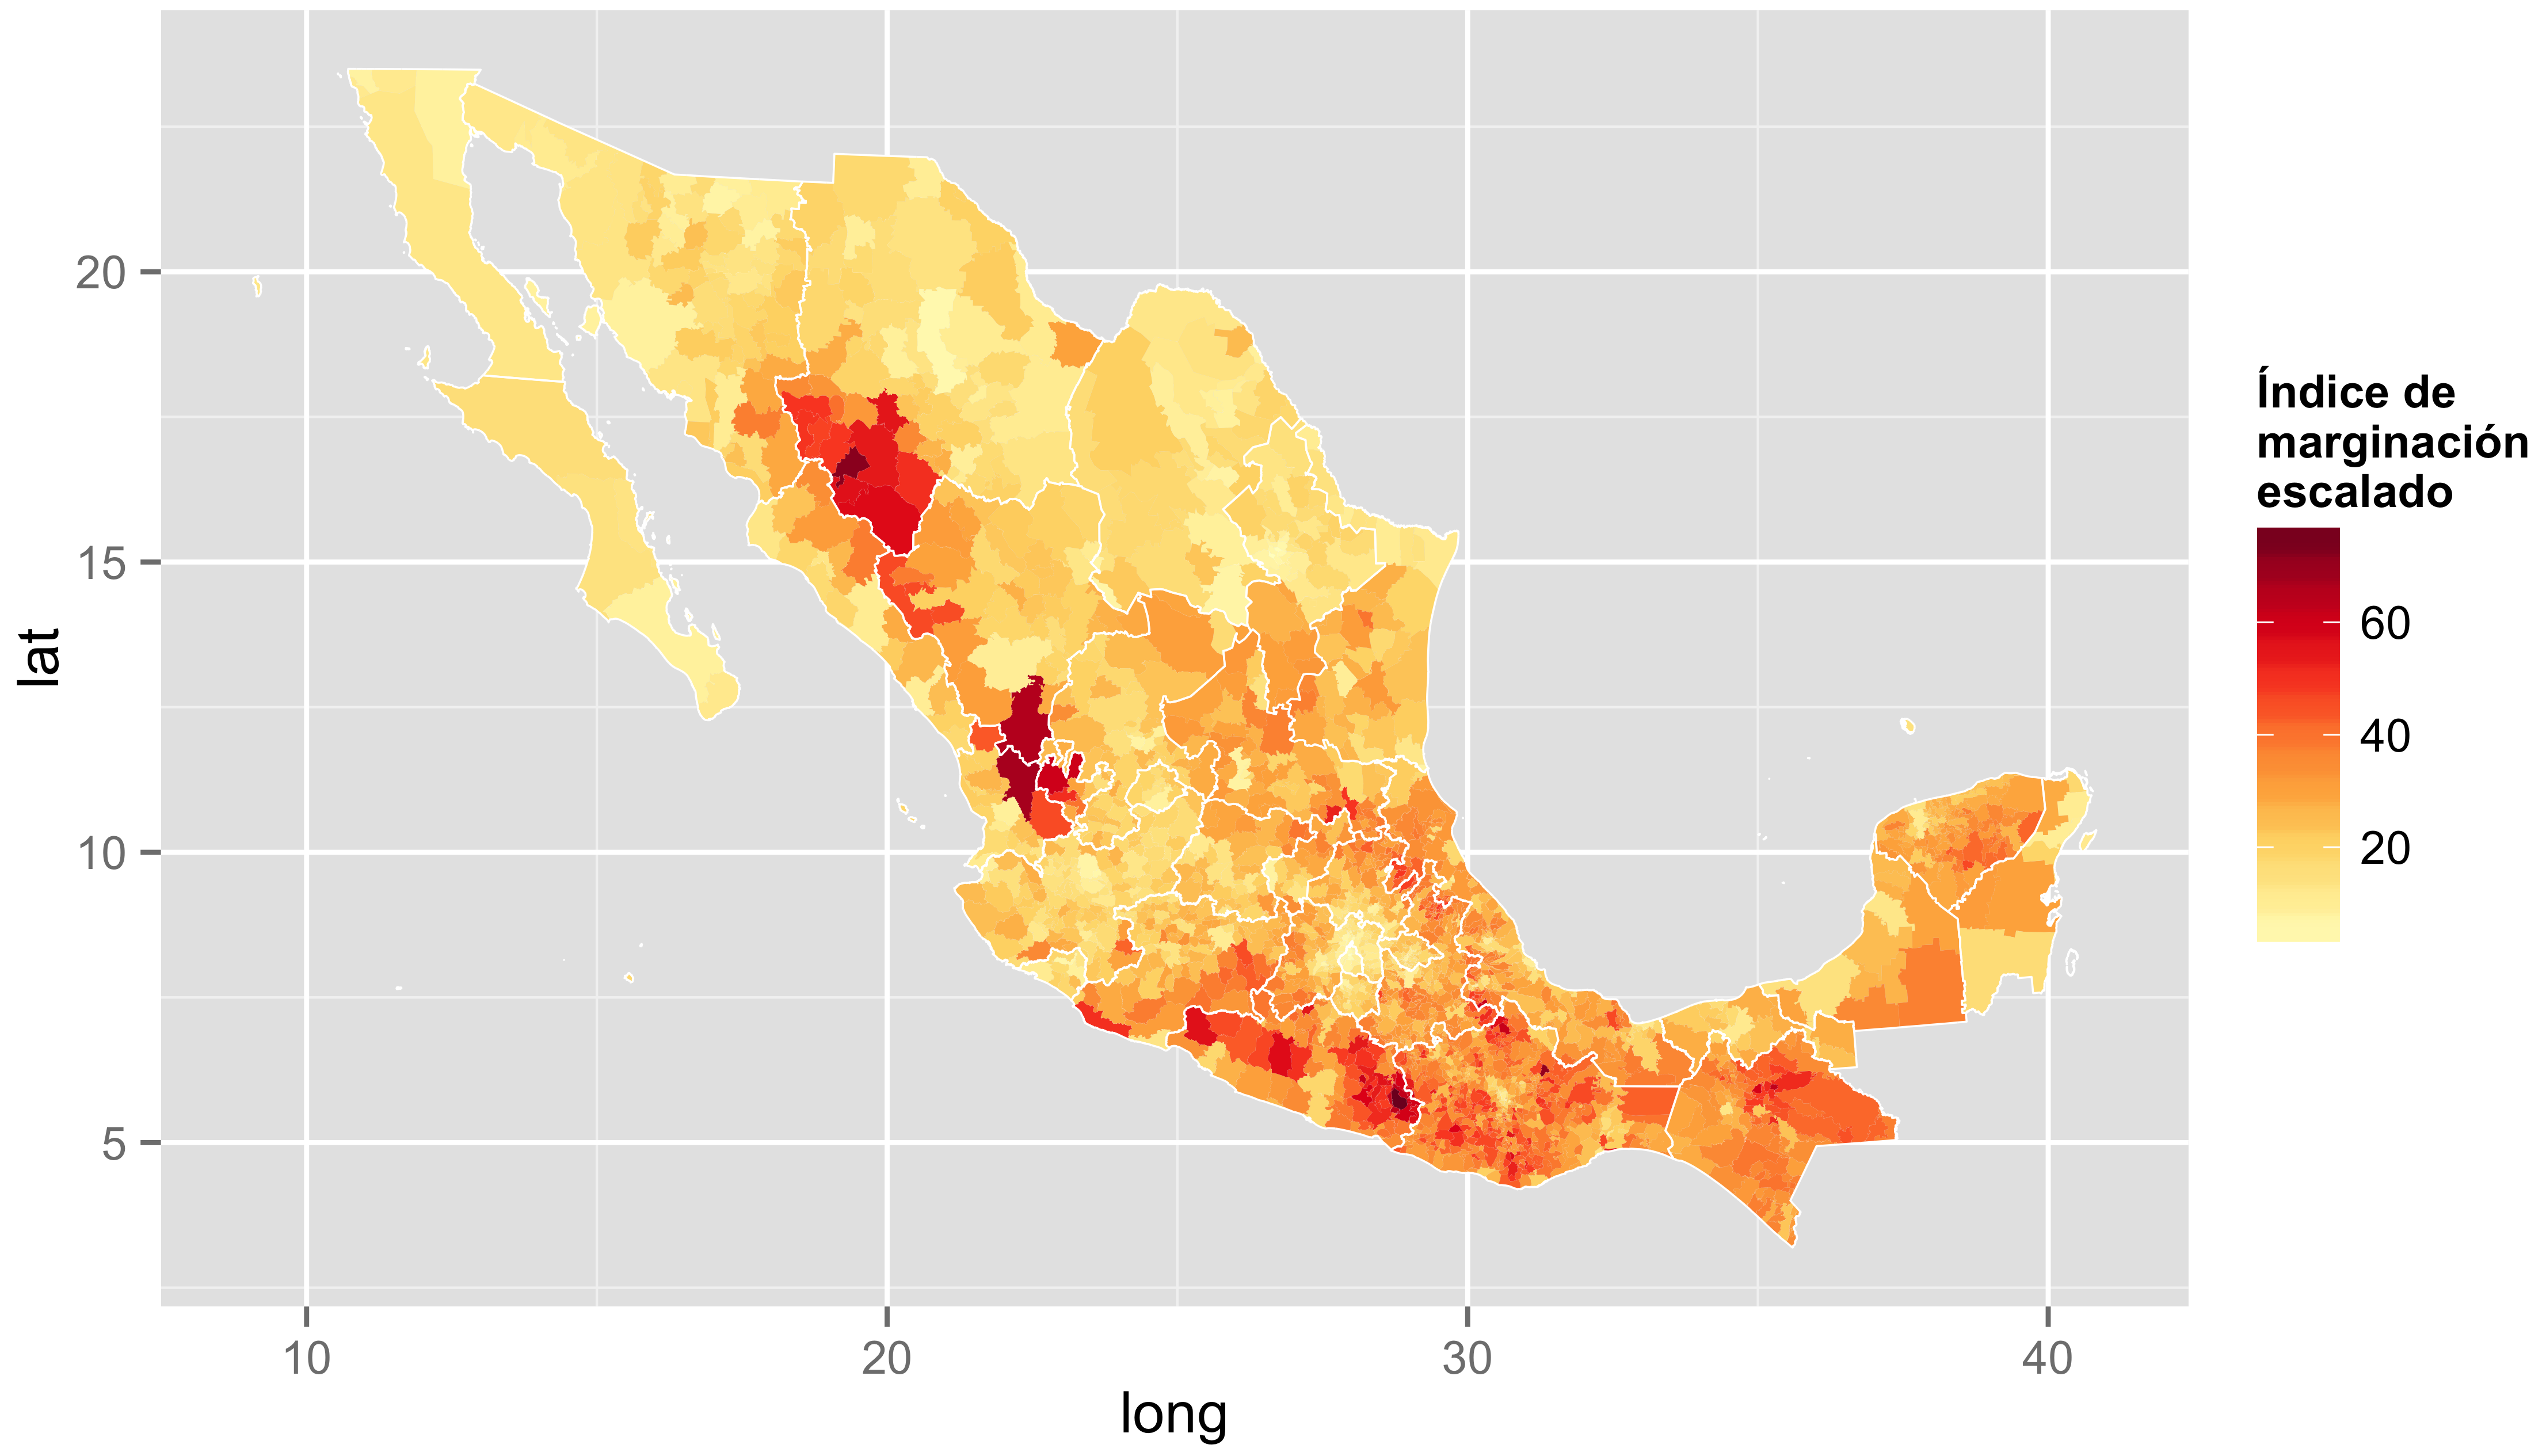
\includegraphics[width=.9\textwidth]{./maps/mapmarg.png} \\
\caption{ Índice de marginación por municipio.}
\label{map_marg_ej}  
\end{figure}

\end{enumerate}

\end{itemize}


\chapter{Autocorrelación Espacial}

Las observaciones realizadas en diferentes puntos espaciales pueden no ser independientes. Por ejemplo, medidas obtenidas en lugares cercanos pueden ser más parecidas que en lugares lejanos. A esto se le llama autocorrelación espacial, la cual mide el grado en el que un fenómeno de interés se relaciona consigo mismo en el espacio \citep{clifford1973, clifford1981}.

Las pruebas de autocorrelación espacial examinan si el valor observado de una variable en algún lugar es independiente de valores de la misma variable en lugares cercanos o  ontiguos.

Un índice de \textit{autocorrelación espacial global} resume el nivel de similitud espacial observada entre las observaciones vecinas sobre el área entera estudiada.

\begin{itemize}
\item \textbf{Autocorrelación espacial positiva} indica que los valores similares están cercanos entre sí, o aglomerados, en el espacio.
\item \textbf{Autocorrelación espacial negativa} indica que valores vecinos no son similares, o equivalentemente, que valores similares están dispersos en el espacio.
\item \textbf{Autocorrelación espacial nula} indica que el patrón espacial es aleatorio.
\end{itemize}

La mayoría de los índices de autocorrelación comparten una estructura común. En dicha estructura, se calcula la similitud entre valores en las localidades $i$ y $j$, luego se pondera dicha similitud por la proximidad entre éstos. Altas similitudes con mucho peso provocan un valor alto del índice, mientras que bajas similitudes con mucho peso provocan un valor bajo del índice.

\section{Matriz de Pesos}
Para evaluar la autocorrelación espacial, se debe definir primero qué significa que dos observaciones sean cercanas, es decir, se debe definir una métrica de distancia. Dichas distancias son presentadas en una matriz de pesos en la cual se define la relación entre los diferentes lugares donde se obtuvieron las observaciones. Si los datos fueron obtenidos en $n$ lugares distintos, entonces la matriz de pesos $W$ es de $n \times n$, donde cada entrada $w_{ij}$, $i,j=1, 2, \dots, n$ representa la dependencia espacial o peso entre los lugares $i$ y $j$ definiendo así la estructura de los vecinos sobre el área entera. \citet{haining} presenta las siguientes maneras para construir los pesos:

\begin{itemize}
\item  \textbf{Contigüidad binaria}: Es la definición de pesos más sencilla, se define como 

\begin{equation} \label{binw}
w_{ij}=  \begin{cases} 1 & \mbox{si la región } i \mbox{ comparte frontera con } j \\ 
0 & \mbox{e.o.c.} 
\end{cases}
\end{equation}.

Nótese que con dicha elección de medida de proximidad $W$ es necesariamente simétrica , pues $w_{ij}=w_{ji}$.


\item \textbf{Distancia}: Se definen los pesos como $w_{ij}=d_{ij}^{-\delta}$ donde $d_{ij}$ denota la distancia entre $i$ y $j$ y el parámetro $\delta \geq 0$. La distancia puede definirse de distintas maneras (e.g. distancia Euclideana).

\item \textbf{Función exponencial de distancia}: Se define como $w_{ij}=e^{d_{ij}^{-\delta}}$.

\item \textbf{Frontera en común}: Sean $l_{ij}$ la longitud de la frontera entre $i$ y $j$ y $l_i$ la longitud de la frontera de la región $i$, se pueden definir los pesos como $w_{ij}=\left( \dfrac{l_{ij}}{l_i}\right)^{\tau}$ con $\tau \geq 0$.

\item \textbf{Combinación de frontera y distancia}: Es una combinación entre los pesos por distancia y por tamaño de frontera, se define como $w_{ij}=\left( \dfrac{l_{ij}}{l_i}\right)^{\tau}d_{ij}^{-\delta}$ donde $\tau, \delta \geq 0$.
\end{itemize}

\textbf{Nota}: Para todos los casos  $w_{ii}=0$ y $w_{ij} \geq 0$ para $i,j=1,2,...,n$, obteniendo así una matriz de la siguiente forma,

\begin{equation}
W= \begin{pmatrix}
 0 & w_{12} & \cdots & w_{1n} \\
 w_{21} & 0 & \cdots & w_{2n}  \\
 \vdots & \vdots & \ddots & \vdots \\
 % w_{n-1,1} & \vdots & \ddots & w_{n-1,n}\\
 w_{n1} & w_{n2} & \cdots & 0  \\
\end{pmatrix}.
\end{equation}

Podemos ajustar $W$ de tal forma que la suma de los pesos por renglón sea igual a $1$  utilizando una matriz estandarizada por filas donde dividimos cada elemento $w_{ij}$ por la suma de los pesos de los vecinos de la región $i$ obteniendo una matriz $W_{std}$ donde

\begin{equation}
w_{std,ij}=\dfrac{w_{ij}}{\displaystyle \sum_{j=1}^n w_{ij}}.
\end{equation}

En el caso de los pesos binarios, dicha estandarización penaliza los pesos de las regiones con muchos vecinos.


\section{Pruebas de Autocorrelación Espacial Global}
Consideremos un área de estudio particionada en $n$ regiones. Sea $Y$ la variable de estudio, $y_i$ es la observación de la variable $Y$ en la región $i$.  Para cada par de regiones $i$ y $j$, si las observaciones $y_i$ y $y_j$ no están correlacionadas, entonces decimos que no hay autocorrelación espacial en el área de estudio para la variable $Y$. De manera inversa, decimos que existe autocorrelación espacial si las observaciones están correlacionadas por pares. Las pruebas de autocorrelación espacial propuestas en la literatura, dependen del tipo de la variable de estudio (discreta, ordinal o continua).

\subsection{Variables continuas u ordinales}
Si $Y$ es de escala continua u ordinal, utilizamos dos coeficientes que miden el grado de autocorrelación entre las $y_i$'s en regiones unidas, donde $y_i$ es una observación en la región $i$.


\subsubsection{Índice $\mathcal{I}$ de Moran} 
El índice $\mathcal{I}$ de Moran propuesto por \citet{moran50} sirve para probar la autocorrelación espacial global para variables continuas. Se basa en los productos cruzados de las desviaciones de la media y se calcula para  $n$ observaciones de una variable $y$ en lugares $i,j$ como sigue:

\begin{equation}
\mathcal{I} = \left( \dfrac{n}{\displaystyle \sum_{i=1}^n \sum_{j=1}^n w_{ij}} \right) \left( \dfrac{\displaystyle \sum_{i=1}^n \sum_{j=1}^n w_{ij} (y_{i} - \bar{y}) (y_{j} - \bar{y}) }{\displaystyle \sum_{i=1}^n (y_{i} - \bar{y})^2} \right).
\end{equation}

$y_{i}$ es el valor de la variable en el lugar $i$ y $\overline{y}$ es la media muestral.

$\mathcal{I}$ no es como un coeficiente de correlación común, pues no pertenece necesariamente al intervalo $(-1,1)$. Usualmente $\mathcal{I} \in (-1,1)$, a menos que se cuente con regiones con valores extremos de $y_{i} - \overline{y}$ con pesos muy altos.


\subsubsection{Índice $\mathcal{C}$ de Geary} 
El índice $\mathcal{C}$ de Geary utiliza la suma de diferencias al cuadrado entre pares de observaciones como medida de variación. Fue sugerido por \citet{geary54} y está dado por

\begin{equation}
\mathcal{C} =  \left(\dfrac{n-1}{\displaystyle 2 \sum_{i=1}^n \sum_{j=1}^n w_{ij}}\right)  \left( \dfrac{\displaystyle \sum_{i=1}^n \sum_{j=1}^n w_{ij} (y_{i} - y_{j})^2}{\displaystyle \sum_{i=1}^n (y_{i} - \hat{y})^2}\right).
\end{equation}

El índice $\mathcal{C}$ de Geary toma valores en el intervalo $[0,2]$ donde 0 indica correlación espacial positiva perfecta (i.e. $y_{i}=y_{j}$ para cualquier par de regiones donde $w_{ij}>0$ y 2 indica correlación espacial negativa perfecta. 

$\mathcal{C}$ no es propiamente un coeficiente de correlación, en cambio, corresponde a una estadístico $d$ de Durbin-Watson \citep{clifford1981}, utilizada para probar autocorrelación serial en análisis de regresión y en análisis de series de tiempo.

En contraste con $\mathcal{I}$ , valores bajos de $\mathcal{C}$ denotan autocorrelación espacial positiva y valores altos indican autocorrelación espacial negativa.


Ambos índices $\mathcal{I}$ y $\mathcal{C}$ tienen la forma clásica de un coeficiente de autocorrelación: el numerador en cada uno es una medida de covarianza entre las $y_i$'s y el denominador es una medida de varianza. Es evidente también que $\mathcal{I}$  está basado en productos cruzados de las desviaciones entre $y_i$ y $\bar{y}$ , opuesto a las diferencias cuadráticas entre las $y_i$'s del coeficiente de Geary.

Se puede mostrar \citep[Capítulo 2]{clifford1973} que  $\mathcal{I}$ y $\mathcal{C}$ asíntóticamente, se distribuyen normal a medida que $n$ aumenta. Los momentos de $\mathcal{I}$ y $\mathcal{C}$ pueden ser evaluados bajo alguna de los siguientes dos supuestos:

\begin{enumerate}
\item \textbf{Normalidad}. Bajo este supuesto, asumimos que las observaciones $y_i$ son resultado de $n$ realizaciones de una población normal.
\item \textbf{Aleatorización}. Independientemente de la distribución subyacente de la población, consideramos el valor observado de $\mathcal{I}$ y $\mathcal{C}$ relativo al conjunto de todos los valores posibles que pueden tomar $\mathcal{I}$ y $\mathcal{C}$ si $y_1, y_2, ..., y_n$ fueran permutadas de manera aleatoria repetidamente alrededor de las regiones dentro del área de estudio. Hay $n!$ valores posibles.
\end{enumerate}

Usando los subíndices N y R para denotar los supuestos de normalidad y aleatorización respectivamente. Si utilizamos pesos $w_{ij}$ simétricos (i.e. $w_{ij}=w_{ji}$) se puede probar que los momentos de los índices quedan como sigue.

\subsubsection*{Coeficiente $\mathcal{I}$}
\begin{align}
\EN\left[\mathcal{I} \right]  = &\ER \left[\mathcal{I}\right]=-\dfrac{1}{n-1},\\
\EN\left[\mathcal{I}^2\right] = & \dfrac{n^2S_1-nS_2+3S_0^2}{S_0^2(n^2-1)}, \\
\ER\left[\mathcal{I}^2\right] = &\dfrac{n \left[ (n^2-3n+3)S_1 - nS_2 + 3S_0^2 \right] - b_2 \left[ (n^2 - n)S_1 - 2nS_2 +6S_0^2\right]}{(n-1)(n-2)(n-3)S_0^2}.
\end{align}

\subsubsection*{Coeficiente $\mathcal{C}$}
\begin{align}
\EN\left[\mathcal{C}\right] = &\left[\mathcal{C}\right] = 1, \\
\VarN(\mathcal{C}) =&\dfrac{(2S_1+S_2)(n-1)-4S_0^2}{2(n+1)S_0^2}, \\
\VarR(\mathcal{C}) =& \Big( (n-1)S_1 \left[ n^2 -3n +3 -(n-1)b_2 \right] \\ \nonumber
   &- \frac{1}{4} (n-1)S_2 \left[ n^2 +3n -6 -(n^2-n+2)b_2 \right] \\ \nonumber
  &+ S_0^2 \left[ n^2 -3 - (n-1)^2 b_2 \right] \Big) \left( \dfrac{1}{n(n-2)(n-1)S_0^2} \right). \nonumber
\end{align}

Donde 
\begin{align}
  S_0 =& \sum_{i=1}^n \sum_{j=1}^n w_{ij}, \\
  S_1 =& \dfrac{1}{2} \sum_{i=1}^n \sum_{j=1}^n  \left( w_{ij}+w_{ji} \right)^2 , \\
  S_2 =& \sum_{i=1}^n  \left( w_{i.}+w_{.i} \right)^2 , 
\end{align}

\begin{eqnarray}
w_{i.} = \sum_{j=1}^n w_{ij} & \mbox{ y } & w_{i.} = \sum_{j=1}^n w_{ij}.
\end{eqnarray}

% Si los pesos son binarios, $S_0 = 2A$,  $S_1=4A$ y $S_2=8(A+D)$.
\textbf{Observación} \label{obs:nrdist}: \citet{hoeffding52} demostró que las distribuciones asintóticas bajo $N$ y $R$ son las mismas bajo condiciones generales razonables. 

\subsection{Variables Discretas: Estadístico join-count (Conteo de fronteras)}\label{subsec:joincountch}

Cuando la variable de interés $y$ es categórica se puede utilizar la estadística join-count para medir el grado de dispersión o conglomeración entre las distintas clases.

Supongamos primero que $y$ cuenta con 2 clases, es decir, es binaria y $y_{i}\in \lbrace 0,1 \rbrace$. Mapeando $y$ en 2 colores , W (blanco por su inicial en inglés) si $y_{i}=0$ y B (negro por su inicial en inglés) cada frontera o unión entre dos regiones es clasificada como $WW$ (0-0), $BB$  (1-1) ó $BW$ (1-0).

Si el número de uniones $BB$ es significativamente mayor del esperado por sorteo, habrá autocorrelación espacial positiva;  si es significativamente menor, autocorrelación espacial negativa; y si es aproximadamente el mismo, autocorrelación espacial nula.

El método de análisis es como sigue \citep{moran48}. El conteo de uniones $BB$ ponderado por $w_{ij}$, está dado por

\begin{equation} \label{bbjoins}
BB = \dfrac{1}{2} \sum_{i=1}^n\sum_{j=1}^n w_{ij} y_i y_j ,
\end{equation}

el número de uniones $BW$ ponderado es

\begin{equation} \label{bwjoins}
BW = \dfrac{1}{2} \sum_{i=1}^n\sum_{j=1}^n w_{ij} (y_i - y_j)^2,
\end{equation}

y el número de uniones $WW$ ponderado es

\begin{equation}
WW = W-(BB+BW),
\end{equation}

donde
\begin{equation} \label{wjoins}
 W = \dfrac{1}{2} \sum_{i=1}^n\sum_{j=1}^n w_{ij} .
\end{equation}

Nótese que utilizando pesos $w_{ij}$ binarios (ver \eqref{binw}) $BB$, $BW$ y $WW$ son el conteo observado de uniones de cada tipo y el factor $\frac{1}{2}$ en \eqref{bbjoins}, \eqref{bwjoins}, \eqref{wjoins} elimina el conteo duplicado, al contar las uniones $ij$ y $ji$ por la propiedad de simetría de los pesos binarios.


El método usual para determinar si $BB$, $BW$ y $WW$ distan significativamente del conteo esperado por sorteo es utilizando el hecho de que dichos estadísticos de conteo de fronteras, asintóticamente se distribuyen $\mathcal{N}(\mu, \sigma^2)$ \citep[Capítulo 2]{clifford1973}. Bajo este enfoque, los parámetros $\mu$ y $\sigma^2$ de los coeficientes pueden ser evaluados bajo uno de las dos supuestos:

\begin{enumerate}
\item \textbf{Muestreo con reemplazo}, donde suponemos que cada una de las regiones es etiquetada como $B$ o $W$ independientemente con probabilidad $p_B$ y $p_W=1-p_B$ respectivamente. 

\item \textbf{Muestreo sin reemplazo}, donde suponemos que cada región tiene la misma probabilidad, a priori, de ser $B$ o $W$, pero la codificación está sujeta a la restricción de que hay $n_B$ regiones con color $B$ y $n_W$ regiones con color $W$, y $n_a+n_b=n$.
\end{enumerate}

Generalmente contamos con más de dos clases ($k > 2$), tenemos que cada una de las $n$ regiones pertenece a alguna de las $k$ categorías. Así, $n_{1}$ regiones son de tipo 1, $n_{2}$ regiones son de tipo 2 y así sucesivamente, y $n_{k}$ regiones son de tipo $k$. De tal manera:
\begin{equation}
n_{1}+n_{2}+...+n_{k}=n.
\end{equation}

Sean $N_{rr}$ el número de uniones entre regiones del tipo $rr$,  $N_{rs}$ el número de uniones del tipo $rs$, con  $r,s \in \{1,2, \dots, k\}$ y $J_{tot}$ el número de fronteras entre todas las regiones de distintas clases. 


Ahora, el análisis procede haciendo el conteo ponderado de fronteras entre regiones de la misma categoría, dos categorías diferentes y todas las regiones de color diferente. Cada una de las distribuciones es evaluada de la manera planteada anteriormente.

Sea $n^{(k)}=n(n-1)(n-2)\dots(n-k+1)$.

Sea $p_r$ la probabilidad de que una región sea de color $r$, los parámetros $\mu$ y $\sigma^2$ están dados por \citet{moran48} como sigue.


\subsubsection*{Muestreo con reemplazo}
Uniones entre regiones del mismo color $N_{rr}$(equivalente a $BB$ para $k=2$)
\begin{equation}
\mu = \dfrac{1}{2} S_0 p_r^2,
\end{equation}
\begin{equation}
\sigma^2 = \dfrac{1}{4} \left[ S_1 p_r^2 + (S_2-2S_1)p_r^3 + (S_1-S_2)p_r^4 \right] .
\end{equation}

Uniones entre regiones de dos colores diferentes $N_{rs}$ (equivalente a $BW$ para $k=2$)
\begin{equation}
\mu = S_0 p_r p_s,
\end{equation}

\begin{equation}
\sigma^2 = \dfrac{1}{4} \left[ 2S_1 p_r p_s + (S_2-2S_1)p_r p_s(p_r+p_s) + 4(S_1-S_2)p_r^2 p_s^2 \right] .
\end{equation}.

Número total de uniones entre regiones de diferentes colores $J_{tot}$ ($k \geq 3$; cuando $k=2$, este caso es igual al número de fronteras $BW$)
\begin{equation}
 \mu = S_0 \sum_{r=1}^{k-1} \sum_{s=r+1}^{k} p_r p_s,
\end{equation}

\begin{align}
\sigma^2 &= \dfrac{S_2}{4} \sum_{r=1}^{k-1} \sum_{s=r+1}^{k} p_r p_s (2S_1-5S_2) \sum_{r=1}^{k-2} \sum_{s=r+1}^{k-1} \sum_{t=s+1}^{k} p_r p_s p_t \\ \nonumber
          & + (S_1-S_2)\left(\sum_{r=1}^{k-1} \sum_{s=r+1}^{k} p_r^2 p_s^2 - 2  \sum_{r=1}^{k-3} \sum_{s=r+1}^{k-3} \sum_{t=s+1}^{k-1} \sum_{u=t+1}^{k}p_r p_s p_t p_u \right) . 
\end{align}

\subsubsection*{Muestreo sin reemplazo}
Uniones entre regiones del mismo color.

\begin{equation}
\mu = \dfrac{S_0n_r(n_r-1)}{2n(n-1)} ,
\end{equation}

\begin{equation}
\sigma^2 = \dfrac{S_1n_r^{(2)}}{4n^{(2)}} + \dfrac{(S_2-2S_1)n_r^{(3)}}{4n^{(3)}} + \dfrac{(S_0^2+S_1-S_2)n_r^{(4)}}{4n^{(4)}}-\mu^2 .
\end{equation}

Uniones entre regiones de dos colores diferentes.
\begin{equation}
\mu = \dfrac{S_0n_r n_s}{n(n-1)},
\end{equation}

\begin{align}
\sigma^2 &=\dfrac{S_1 n_r n_s}{2n^{(2)}} +  \dfrac{(S_2-2S_1)n_r n_s(n_r+n_s-2)}{4n^{(3)}} \\ \nonumber
         &+ \dfrac{(S_0^2+S_1-S_2)n_r^{(2)}n_s^{(2)}}{n^{(4)}}-\mu^2 .
\end{align}

Número total de uniones entre regiones de diferentes colores
\begin{equation}
\mu = S_0 \sum_{r=1}^{k-1} \sum_{s=r+1}^{k} \dfrac{n_r n_s}{n^{(2)}},
\end{equation}

\begin{align}
&\sigma^2 = \left[ \dfrac{S_2}{4n^{(2)}} - \dfrac{(S_0^2 + S_1 - S_2)(n-1)}{4n^{(4)}} \right]\sum_{r=1}^{k-1} \sum_{s=r+1}^{k} n_r n_s \\ \nonumber
        & + \left[ \dfrac{(S_1 - S_2)}{n^{(4)}} + \dfrac{S_0^2(2n-3)}{n^{(2)}n^{(4)}} \right] \sum_{r=1}^{k-1} \sum_{s=r+1}^{k} n_r^2 n_s^2 \\ \nonumber
        & + \left[ \dfrac{2S_1 - 5S_2}{2n^{(3)}} + \dfrac{3(S_0^2+S_1-S_2)}{n^{(4)}} + \dfrac{2S_0^2}{n^{(3)}(n-1)} \right] \sum_{r=1}^{k-2} \sum_{s=r+1}^{k-1} \sum_{t=s+1}^{k} n_r n_s n_t  \\ \nonumber
        & - 2 \left[ \dfrac{S_1-S_2}{n^{(4)}}+ \dfrac{2S_0^2(2n-3)}{n^{(2)}n^{(4)}} \right]  \sum_{r=1}^{k-3} \sum_{s=r+1}^{k-2} \sum_{t=s+1}^{k-1} \sum_{u=t+1}^{k}n_r n_s n_t n_u . 
\end{align}


\subsection{Pruebas de hipótesis}
La hipótesis nula $H_0$ es de no autocorrelación espacial, es decir, de aleatoriedad espacial:
\begin{itemize}
\item Los valores observados en cierta región, no dependen de los valores observados en regiones vecinas.
\item El patrón espacial observado es igual de probable que cualquier otro patrón espacial.
\item La ubicación de los valores puede ser alterada sin alterar el contenido de información de los datos.
\end{itemize}


Hay dos procedimientos a seguir de acuerdo al supuesto bajo el que estamos trabajando.


\subsubsection{Bajo el supuesto de normalidad}
  \begin{itemize}
    \item \textbf{Conteo de fronteras} \\
    Utilizando el estadístico de conteos del mismo color $N_{rr}$, $r \in \{ 1,2, \dots, k\}$ podemos hacer una prueba cada una de las categorías de manera independiente, obteniendo $k$ pruebas distintas. El estadístico de prueba es 
    \begin{equation}
    z = \dfrac{N_{rr} - \mu}{\sqrt{\sigma^2}} \sim \mathcal{N}(0, 1).
    \end{equation}
   
    Se calculan $\mu$ y $\sigma^2$ de acuerdo al supuesto bajo el que estemos trabajando. Utilizamos el supuesto de muestreo con reemplazo si las $p_i$'s son conocidas a priori. Si dichas probabilidades son estimadas a partir de los datos por $\frac{n_i}{n}$ $(i=1, 2, \dots, k)$ debemos utilizar muestreo sin reemplazo.

    También podemos probar sobre $N_{rs}$ ó $J_{tot}$.
    \item \textbf{Estadísticos $\mathcal{I}$ y $\mathcal{C}$} \\
    De igual manera que el punto anterior, utilizamos un estadístico $z$. Para $\mathcal{I}$ calculamos

    \begin{equation}
    z = \dfrac{\mathcal{I} - \E[\mathcal{I}]}{\sqrt{\Var(\mathcal{I})}},
    \end{equation}

    mientras que para $\mathcal{C}$
    \begin{equation}\label{eq:zgeary}
    z = \dfrac{\E[\mathcal{C}]-\mathcal{C}}{\sqrt{\Var(\mathcal{C})}}.
    \end{equation}

    Recordemos que el coeficiente de Geary está construido de tal forma que, bajo $H_0$, $c=1$; valores de  $\mathcal{C}<1$ indican autocorrelación espacial positiva; y valores de  $\mathcal{C}<1$ indican autocorrelación espacial negativa. Entonces, calculamos $\E[\mathcal{C}]-\mathcal{C}$ en vez de $\mathcal{C}-\E[\mathcal{C}]$ de tal forma que valores positivos del estadístico correspondan a autocorrelación espacial positiva, y valores negativos a autocorrelación espacial negativa.

    Nótese que podemos utilizar dicho estadístico de prueba para cualquiera de los dos supuestos de normalidad y aleatorización ya que, asíntoticamente y bajo condiciones regulares tienen la misma distribución (ver \ref{obs:nrdist}).
  \end{itemize}

  \subsubsection{Simulaciones de Monte Carlo}\label{sec:montecarlo}
    Si dudamos del supuesto de normalidad, podemos utilizar simulaciones de Monte Carlo para examinar la forma de la función de densidad de los coeficientes de autocorrelación espacial bajo la hipótesis nula. 

    Es recomendable hacer esta prueba ya que la función de densidad del estadístico es sensible a los siguientes factores  \citep{clifford1981}:
    \begin{enumerate}
    \item La forma de las regiones en el área de estudio y el número promedio de fronteras por región.
    \item Los pesos $w_{ij}$ utilizados.
    \item La distribución de la variable $Y$.
    \item El tamaño de la muestra $n$.
    \end{enumerate} 

    El proceso de muestreo es el siguiente:
    \begin{enumerate}
    \item Permutamos aleatoriamente las etiquetas $y_1, y_2, \dots, y_n$ a través de las regiones. Por ejemplo, el mapa \ref{rmap_marg_ej} es una permutación aleatoria del mapa \ref{map_marg_ej}.
    \begin{figure}[!ht]
      \centering
      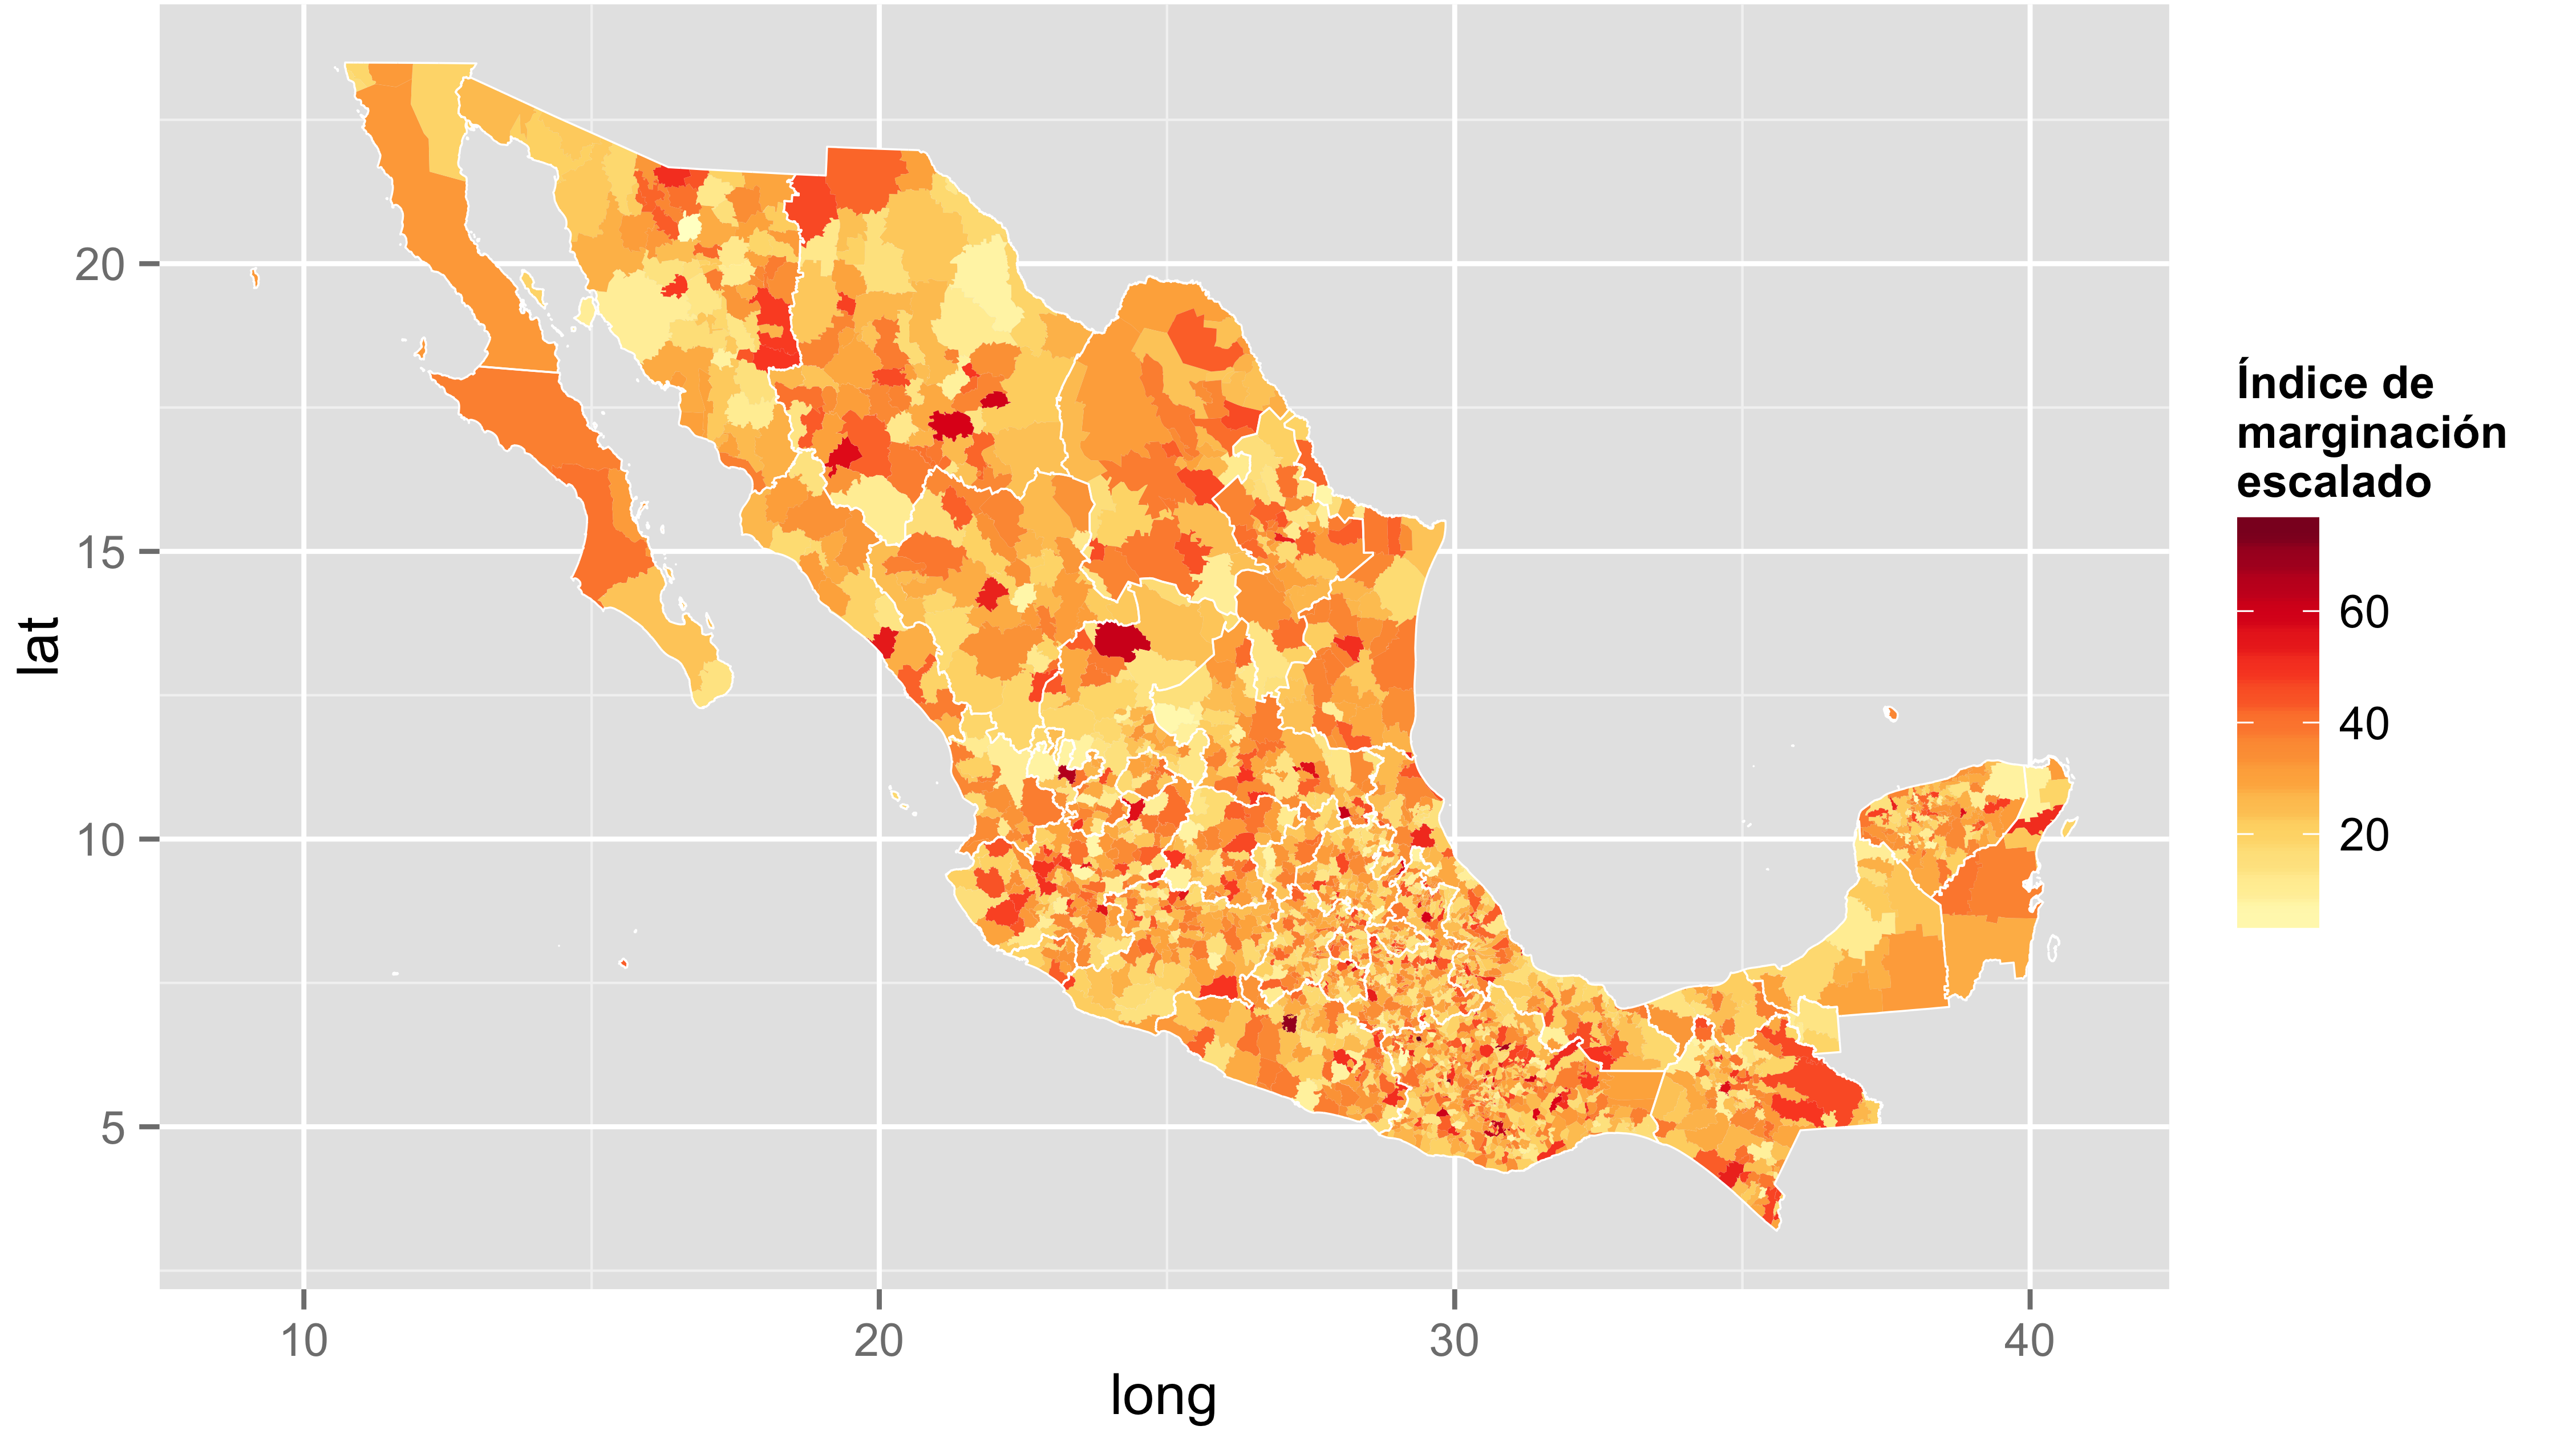
\includegraphics[width=\textwidth]{./maps/rmapmarg.png} \\
      \caption{ Permutación aleatoria del índice de marginación por municipio.}
      \label{rmap_marg_ej}  
    \end{figure}

    \item Calculamos el estadístico de interés, digamos $\mathcal{I}$, con las etiquetas permutadas. Si la variable $Y$ es continua hay $n!$ permutaciones posibles; si es discreta, $\dbinom{n}{n_1 n_2 \dots n_k}$.
    \item Repetimos 1. y 2. $n_{sim}$ veces, obteniendo una muestra de tamaño $n_{sim}$ de $\mathcal{I}$. 
    \item Comparamos el valor observado del estadístico con la muestra obtenida. Si la hipótesis alternativa. Si la $\mathcal{I}$ observada cae en un área mayor a $(1-\alpha)\%$ o menor a $\alpha\%$, entonces $\mathcal{I}$ es significativamente (positivo o negativo) a un nivel de significancia $\alpha$.
    \end{enumerate}


\subsection{Diagrama de dispersión de Moran} 
Un enfoque para visualizar asociación espacial se basa en el concepto del diagrama de dispersión de Moran propuesto por \citet{anselin93} que compara la variable de interés $y_i$  contra su retraso espacial (promedio ponderado de $Y$ en las regiones vecinas de $i$), para $i=1,2,\dots,n$. 

Si restamos $\bar{y}$ a ambos valores, la nube queda partida por los ejes en cuatro cuadrantes. Puntos en los cuadrantes Alto-Alto y Bajo-Bajo indican autocorrelación espacial positiva; mientras que puntos los cuadrantes Alto-Bajo y Bajo-Alto, autocorrelación espacial negativa.

Si colocamos el retraso espacial en el eje vertical y el valor en cada región en el eje de horizontal, el índice $\mathcal{I}$ corresponde a la pendiente de la línea de regresión ajustada.



\part{Resultados y Conclusión}
%%%%%%%%%%%%%%%%%%%%%%%%%%%%%%%%%%%%%%%%%%%%%%%%%%%%%%%%%%%%%%%%%%% 
%                                                                 %
%                         Capítulo 3                           %
%                                                                 %
%%%%%%%%%%%%%%%%%%%%%%%%%%%%%%%%%%%%%%%%%%%%%%%%%%%%%%%%%%%%%%%%%%% 

\chapter{Resultados}

\section{Descripción de la base}
  
La información sobre la cual se trabajó corresponde a la base de datos de CONAPO (Consejo Nacional de Población): ``Índice de Marginación por Entidad Federativa y Municipio 2010''. La base cuenta con $2,456$ observaciones y cada una tiene $15$ atributos descritos en la tabla \ref{descripvar} que corresponden a variables para medir el grado de marginación de un municipio.  

Para cada observación, se cuenta con un polígono geolocalizado que corresponde a la forma del municipio o delegación. Entonces, nuestra área de estudio espacial es la República Mexicana, que  corresponde a una retícula irregular, donde cada región corresponde a un municipio.

\begin{table}
\caption[Descripción de la base de datos]
            {Leyenda variables de marginación 2010.}
\label{descripvar}
\begin{tabular}{l p{10cm} r}
\hline
Variable & Descripción \\
\hline 
clave\_ent & Clave de la entidad federativa  \\	
clave\_mun & Clave de municipio	\\
nom\_mun	& Nombre del municipio \\
poblac & Población total \\
analf & \% de Población de 15 años o más analfabeta  \\ 
sprim & \%  de Población de 15 años o más sin primaria completa  \\ 
sdren  & \% Ocupantes en viviendas sin drenaje ni excusado  \\ 
selec & \% Ocupantes en viviendas sin energía eléctrica  \\ 
sagua & \% Ocupantes en viviendas sin agua entubada  \\ 
hacina & \% Viviendas con algún nivel de hacinamiento \\ 
pisot & \% Ocupantes en viviendas con piso de tierra  \\ 
pl5khab & \% Población en localidades con menos de 5 000 habitantes  \\ 
bingreso & \% Población ocupada con ingreso de hasta 2 salarios mínimos \\ 
imarg & Índice de marginación  \\ 
gmarg & Grado de marginación  \\ 
imarges & Índice de marginación escalado de 0 a 100  \\
lugar & Lugar que ocupa a nivel nacional \\
\hline 
\end{tabular} 
\end{table}

Las variables analf, sprim, sdren, selec, sagua, hacina, pisot, l5khab y bingreso son indicadores de marginación definidos por \citet{conapo04} (Consejo Nacional de Población) que miden el nivel de marginación en cuatro dimensiones: educación, vivienda, distribución de la población e ingresos monetarios. 

El valor del índice de marginación es la primera componente del método de componentes principales, aplicado a los nueve indicadores mencionados; una vez determinados los
valores para cada área, se clasifican en cinco grupos diferenciados y delimitados mediante la técnica de estratificación óptima de Dalenius y Hodges \citep{conapo11}.

\section{Análisis Exploratorio}


Empezamos observando el diagrama de dispersión  de Moran \ref{obj:moranplot} que compara el índice de marginación de un municipio contra el promedio de índice de marginación de sus vecinos, podemos observar que hay una correlación positiva muy alta. Esto es un síntoma de autocorrelación espacial positiva, pues esperamos valores parecidos de índice de marginación entre vecinos. 

Los puntos que están por arriba de la nube de puntos tienen menor índice de marginación con respecto a sus vecinos; en contraste, puntos por debajo de la nube, tienen mayor índice de marginación con respecto a sus vecinos.

Se realizó una regresión lineal simple para encontrar aquellas observaciones cuyos residuales son altos. 

\begin{figure}[!ht]
\centering
% 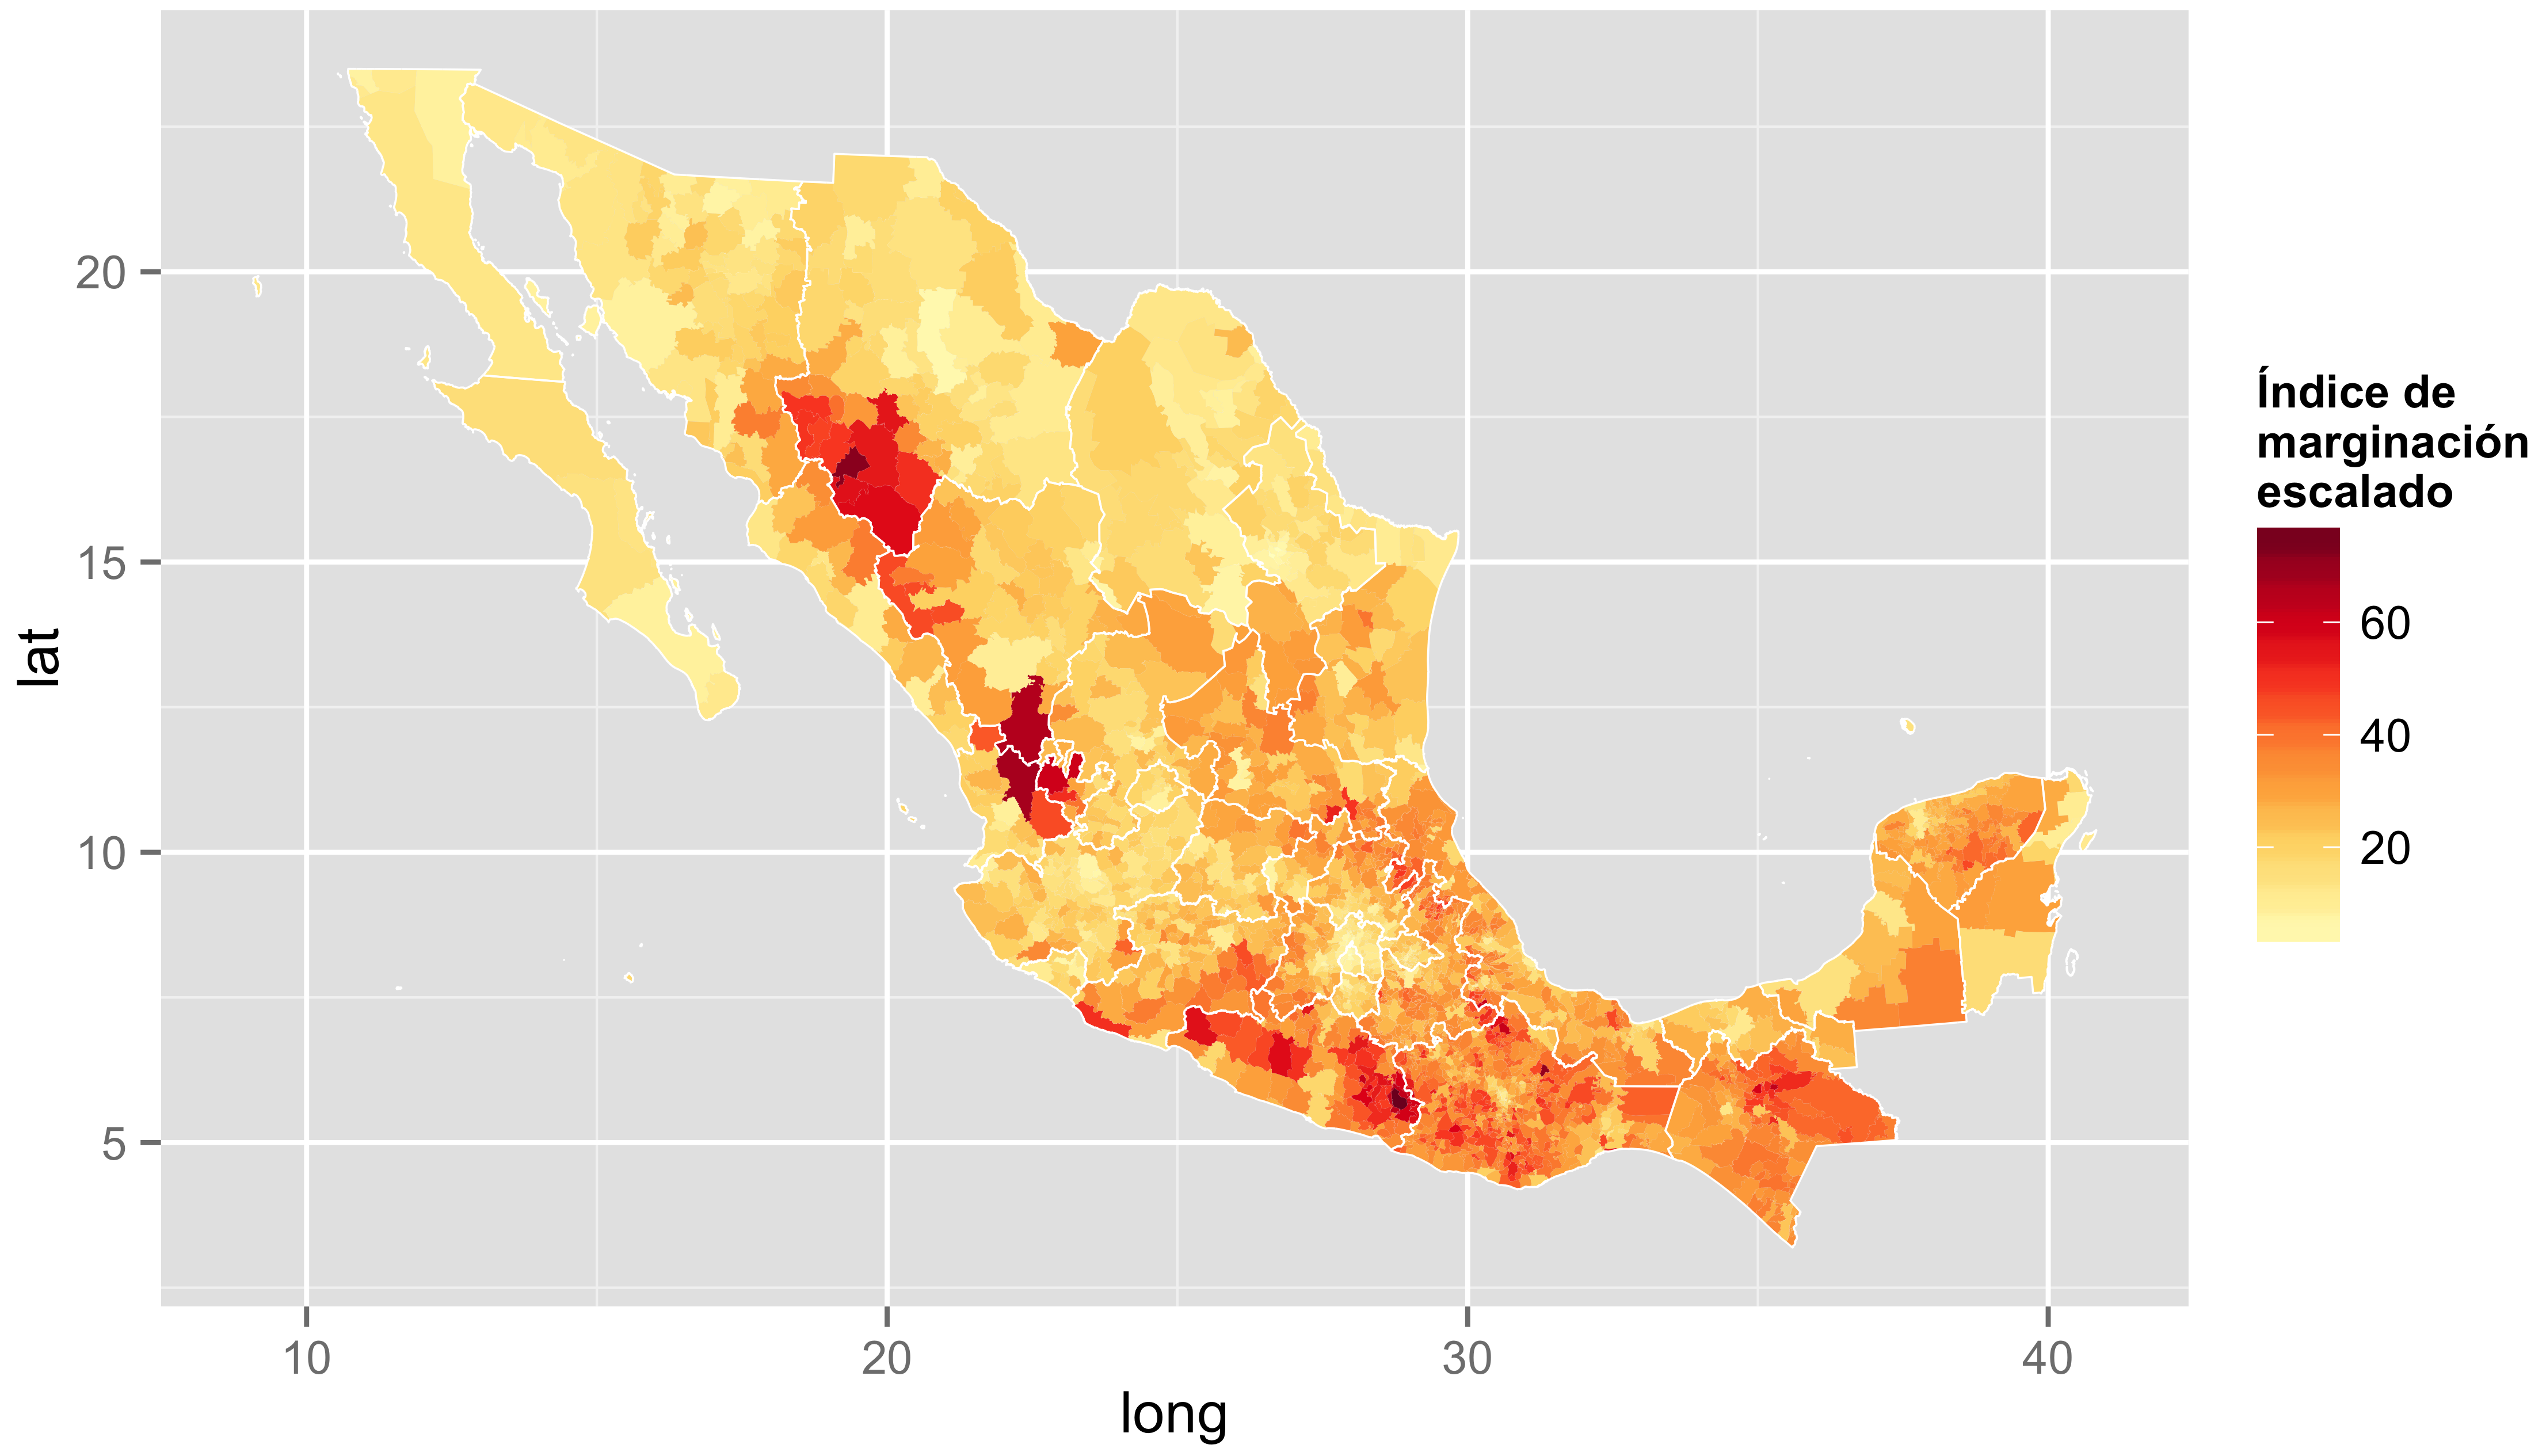
\includegraphics[scale=.20]{./maps/mapmarg.png} \\
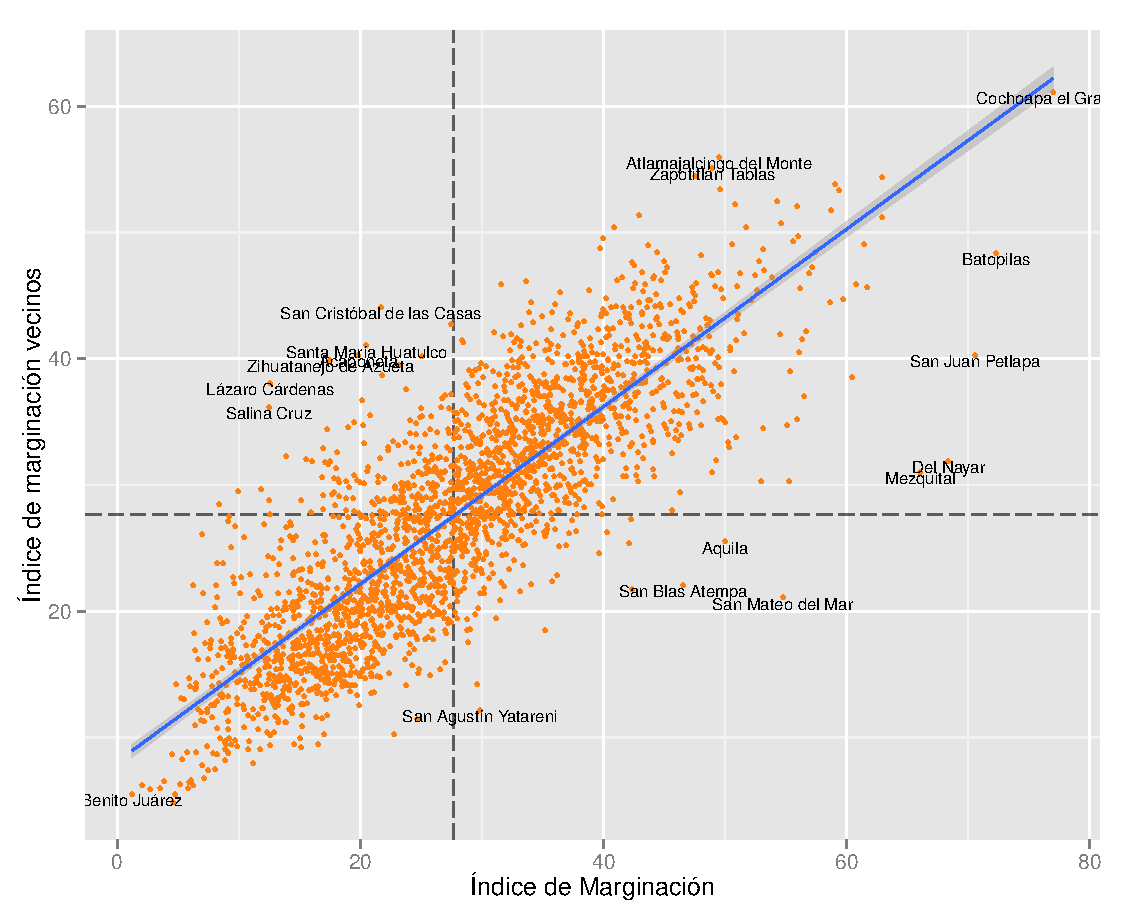
\includegraphics[width=.95\textwidth]{./plots/moran_plot.pdf} \\
\caption{Gráfica de Moran para índice de marginación.}
\label{obj:moranplot}  
\end{figure}

Algunos casos interesantes son los siguientes:
\begin{itemize}
\item Podemos ver que San Mateo del Mar está muy lejos y por debajo de la nube de puntos, su índice de marginación es muy alto en comparación con el de sus vecinos. En contraste, vemos en la parte de arriba a la izquierda al municipio de Salina Cruz, que tiene un índice de marginación más bajo. De hecho, ambos municipios son vecinos en el estado de Oaxaca. Salina Cruz es un importante centro industrial, debido a la presencia de la Refinería Ing. Antonio Dovalí Jaime de PEMEX.

\item Otros municipios que se encuentran muy por debajo de la curva, son Mezquital, en Durango y Del Nayar, en Nayarit. Estos municipios ocupan el quinto y el tercer lugar de marginación a nivel nacional respectivamente. Aunque estén en estados diferentes, ambos municipios comparten frontera y por lo tanto, tienes características similares. Los dos son municipios que se mantuvieron al margen de la evolución ocurrida en el resto de su entidad correspondiente, por la concentración de población indígena. Ambos ocupan el primer lugar de marginación dentro de su entidad. Se pueden apreciar en el mapa ~\ref{obj:mapmarg} de color rojo intenso, al sur de Durango y norte de Nayarit.

\item En el caso de San Cristobal de las Casas, está por arriba de la nube de puntos. Es el municipio de Chiapas con menor índice de marginación. Esto se puede deber al turismo y a las inversiones en la región. 
\end{itemize}

El mapa coroplético \ref{obj:mapmarg} muestra de manera clara que hay una alta autocorrelación espacial positiva en el índice de marginación. Se puede observar que en general hay una transición suave entre colores obscuros y claros, es decir, entre municipios vecinos hay colores muy parecidos, lo que indica valores de marginación cercanos.  

Encontramos puntos rojos obscuros de alta marginación en lugares como la Sierra Tarahumara al suroeste de Chihuahua, sur de Durango y norte de Nayarit (Mezquital y Del Nayar), límites entre Puebla y Veracruz,  los estados de Oaxaca, Guerrero y Chiapas, etc.

\begin{landscape}
\begin{figure}[!ht]
\centering
% 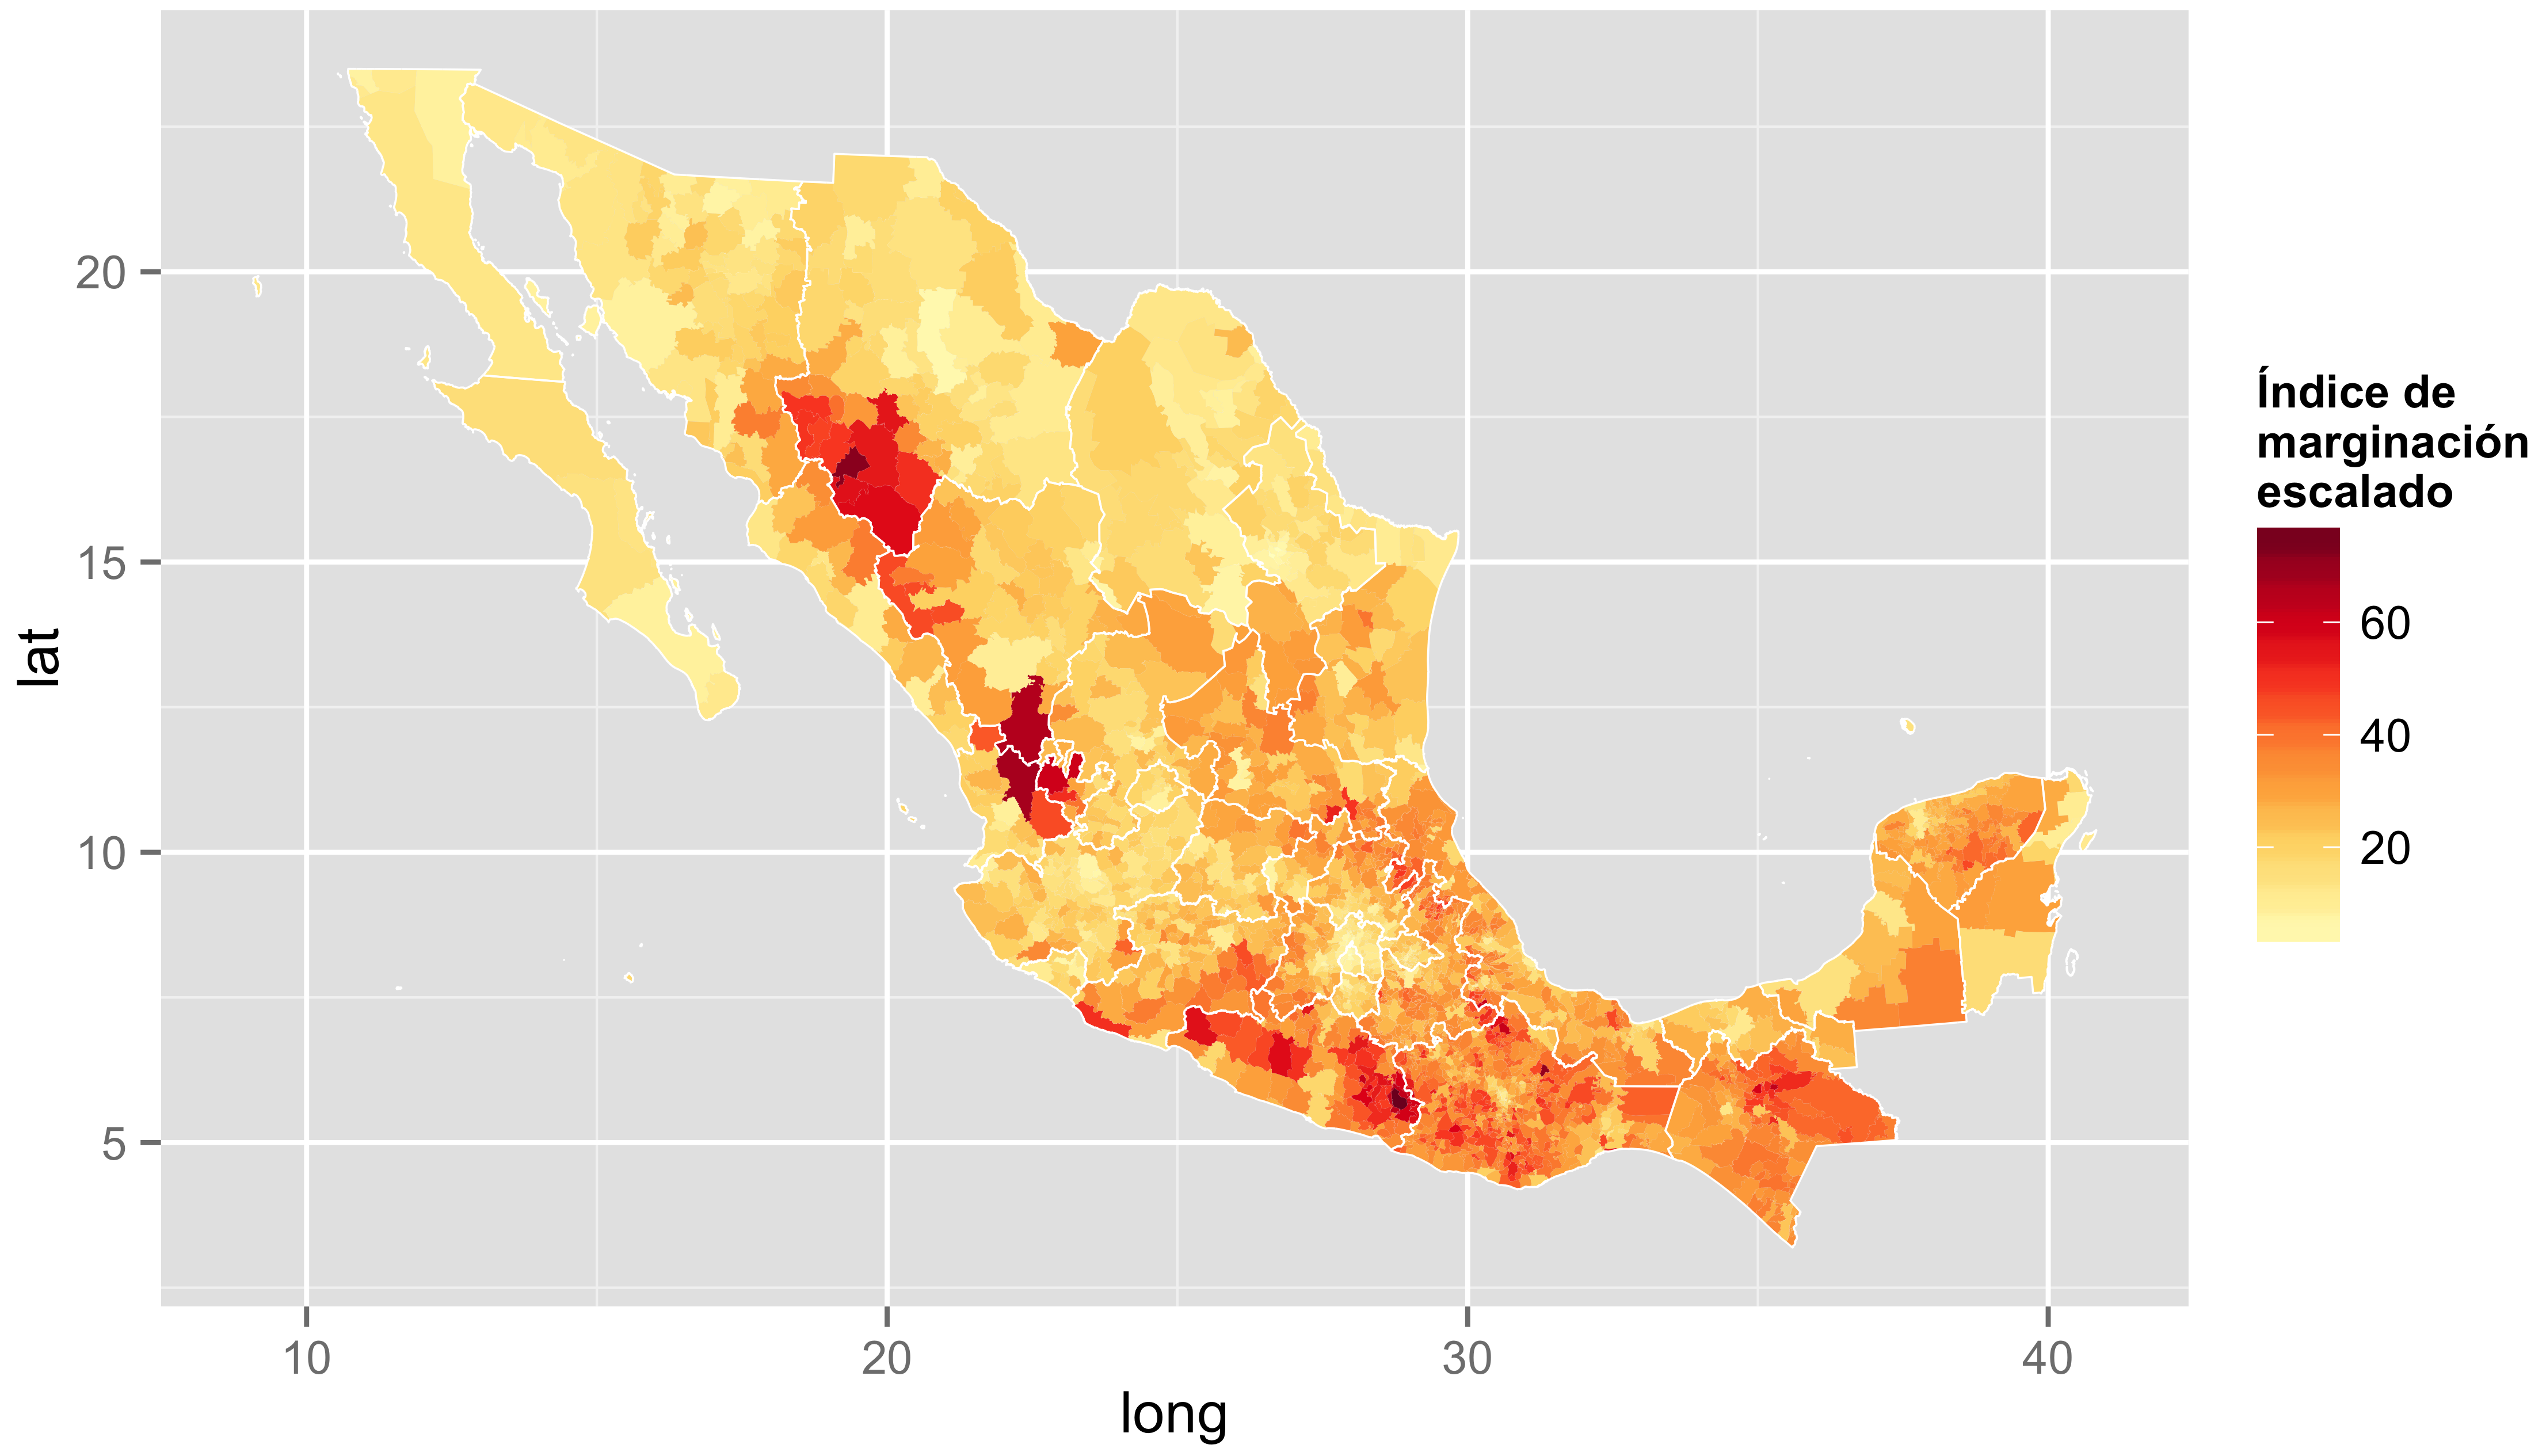
\includegraphics[scale=.20]{./maps/mapmarg.png} \\
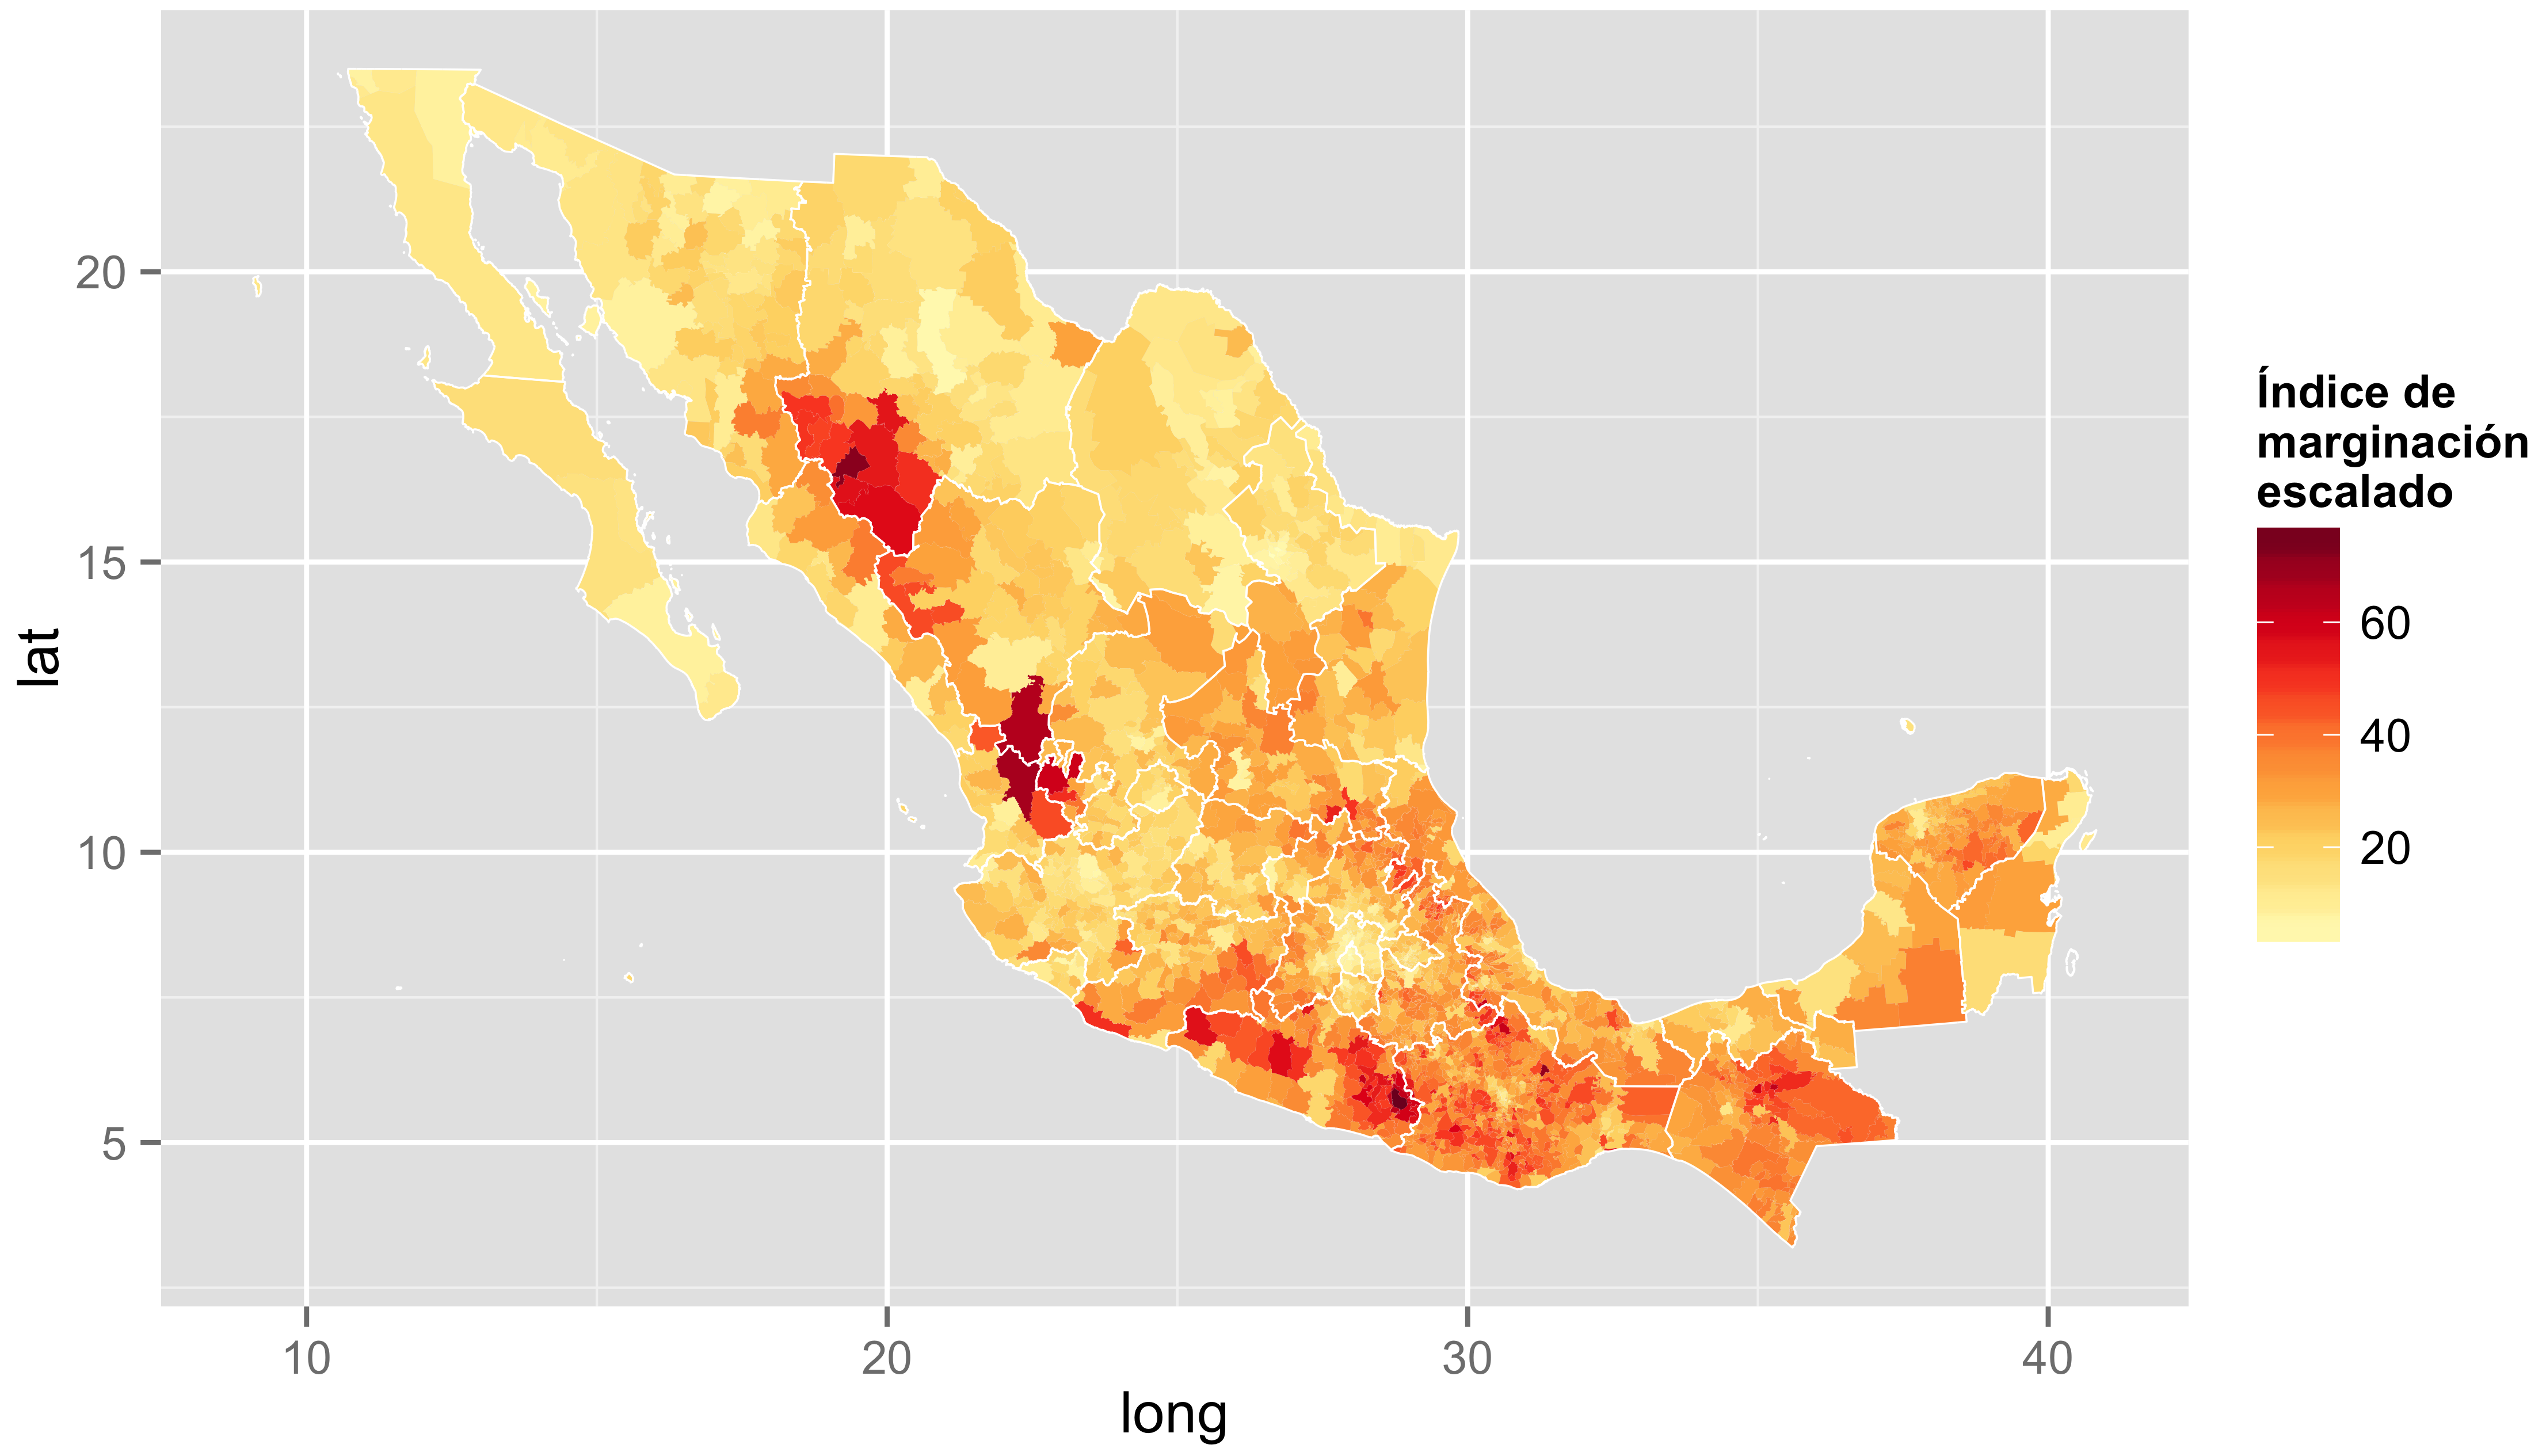
\includegraphics[width=1.4\textheight]{./maps/mapmarg.png} \\
\caption{Mapa de México coloreando cada municipio por su índice de marginación.}
\label{obj:mapmarg}  
\end{figure}
\end{landscape}

Las tabla \ref{tab:masmarg}  muestra los municipios más marginados. Aparecen los casos de Mezquital y Del Nayar mencionados anteriormente. Batopilas es un municipio que se encuentra en la Sierra Tarahumara en Chihuahua; San Juan Petlapa, en Oaxaca y  Cochoapa el Grande, el municipio más marginado, en Guerrero.

\begin{table}[ht]
\centering
\begin{tabular}{llrl}
  \hline
nom\_mun & gmarg & imarges & lugar \\ 
  \hline
  Cochoapa el Grande & Muy alto & 76.98 & 1 \\
  Batopilas & Muy alto & 72.27 & 2 \\ 
  San Juan Petlapa & Muy alto & 70.55 & 3 \\ 
  Del Nayar & Muy alto & 68.38 & 4 \\
  Mezquital & Muy alto & 66.06 & 5 \\ 
   \hline
\end{tabular}
\caption[Municipios más marginados]
            {Tabla de municipios más marginados,}
\label{tab:masmarg}
\end{table}



La lista de los municipios menos marginados se encuentra en la tabla \ref{tab:menosmarg}. Destacan tres delegaciones del Distrito Federal (Coyoacán, Miguel Hidalgo y Benito Juárez)  y dos municipios que forman parte de la zona metropolitana de la Ciudad de Monterrey en Nuevo León (San Pedro Garza García y San Nicolás de los Garza).

\begin{table}[ht]
\centering
\begin{tabular}{llrl}
  \hline
nom\_mun & gmarg & imarges & lugar \\ 
  \hline
  Coyoacán & Muy bajo & 3.86 & 2,452 \\ 
  Miguel Hidalgo & Muy bajo & 3.56 & 2,453 \\   
  San Nicolás de los Garza & Muy bajo & 2.69 & 2,454 \\ 
  San Pedro Garza García & Muy bajo & 2.09 & 2,455 \\
  Benito Juárez & Muy bajo & 1.21 & 2,456 \\ 
  \hline
\end{tabular}
\caption[Municipios menos marginados]
            {Tabla de municipios menos marginados.}
\label{tab:menosmarg}
\end{table}

En la gráfica~\ref{obj:gradosmarg} se presenta el conteo de municipios por nivel de grado de marginación por estado.

\begin{figure}[!ht]
\centering
% 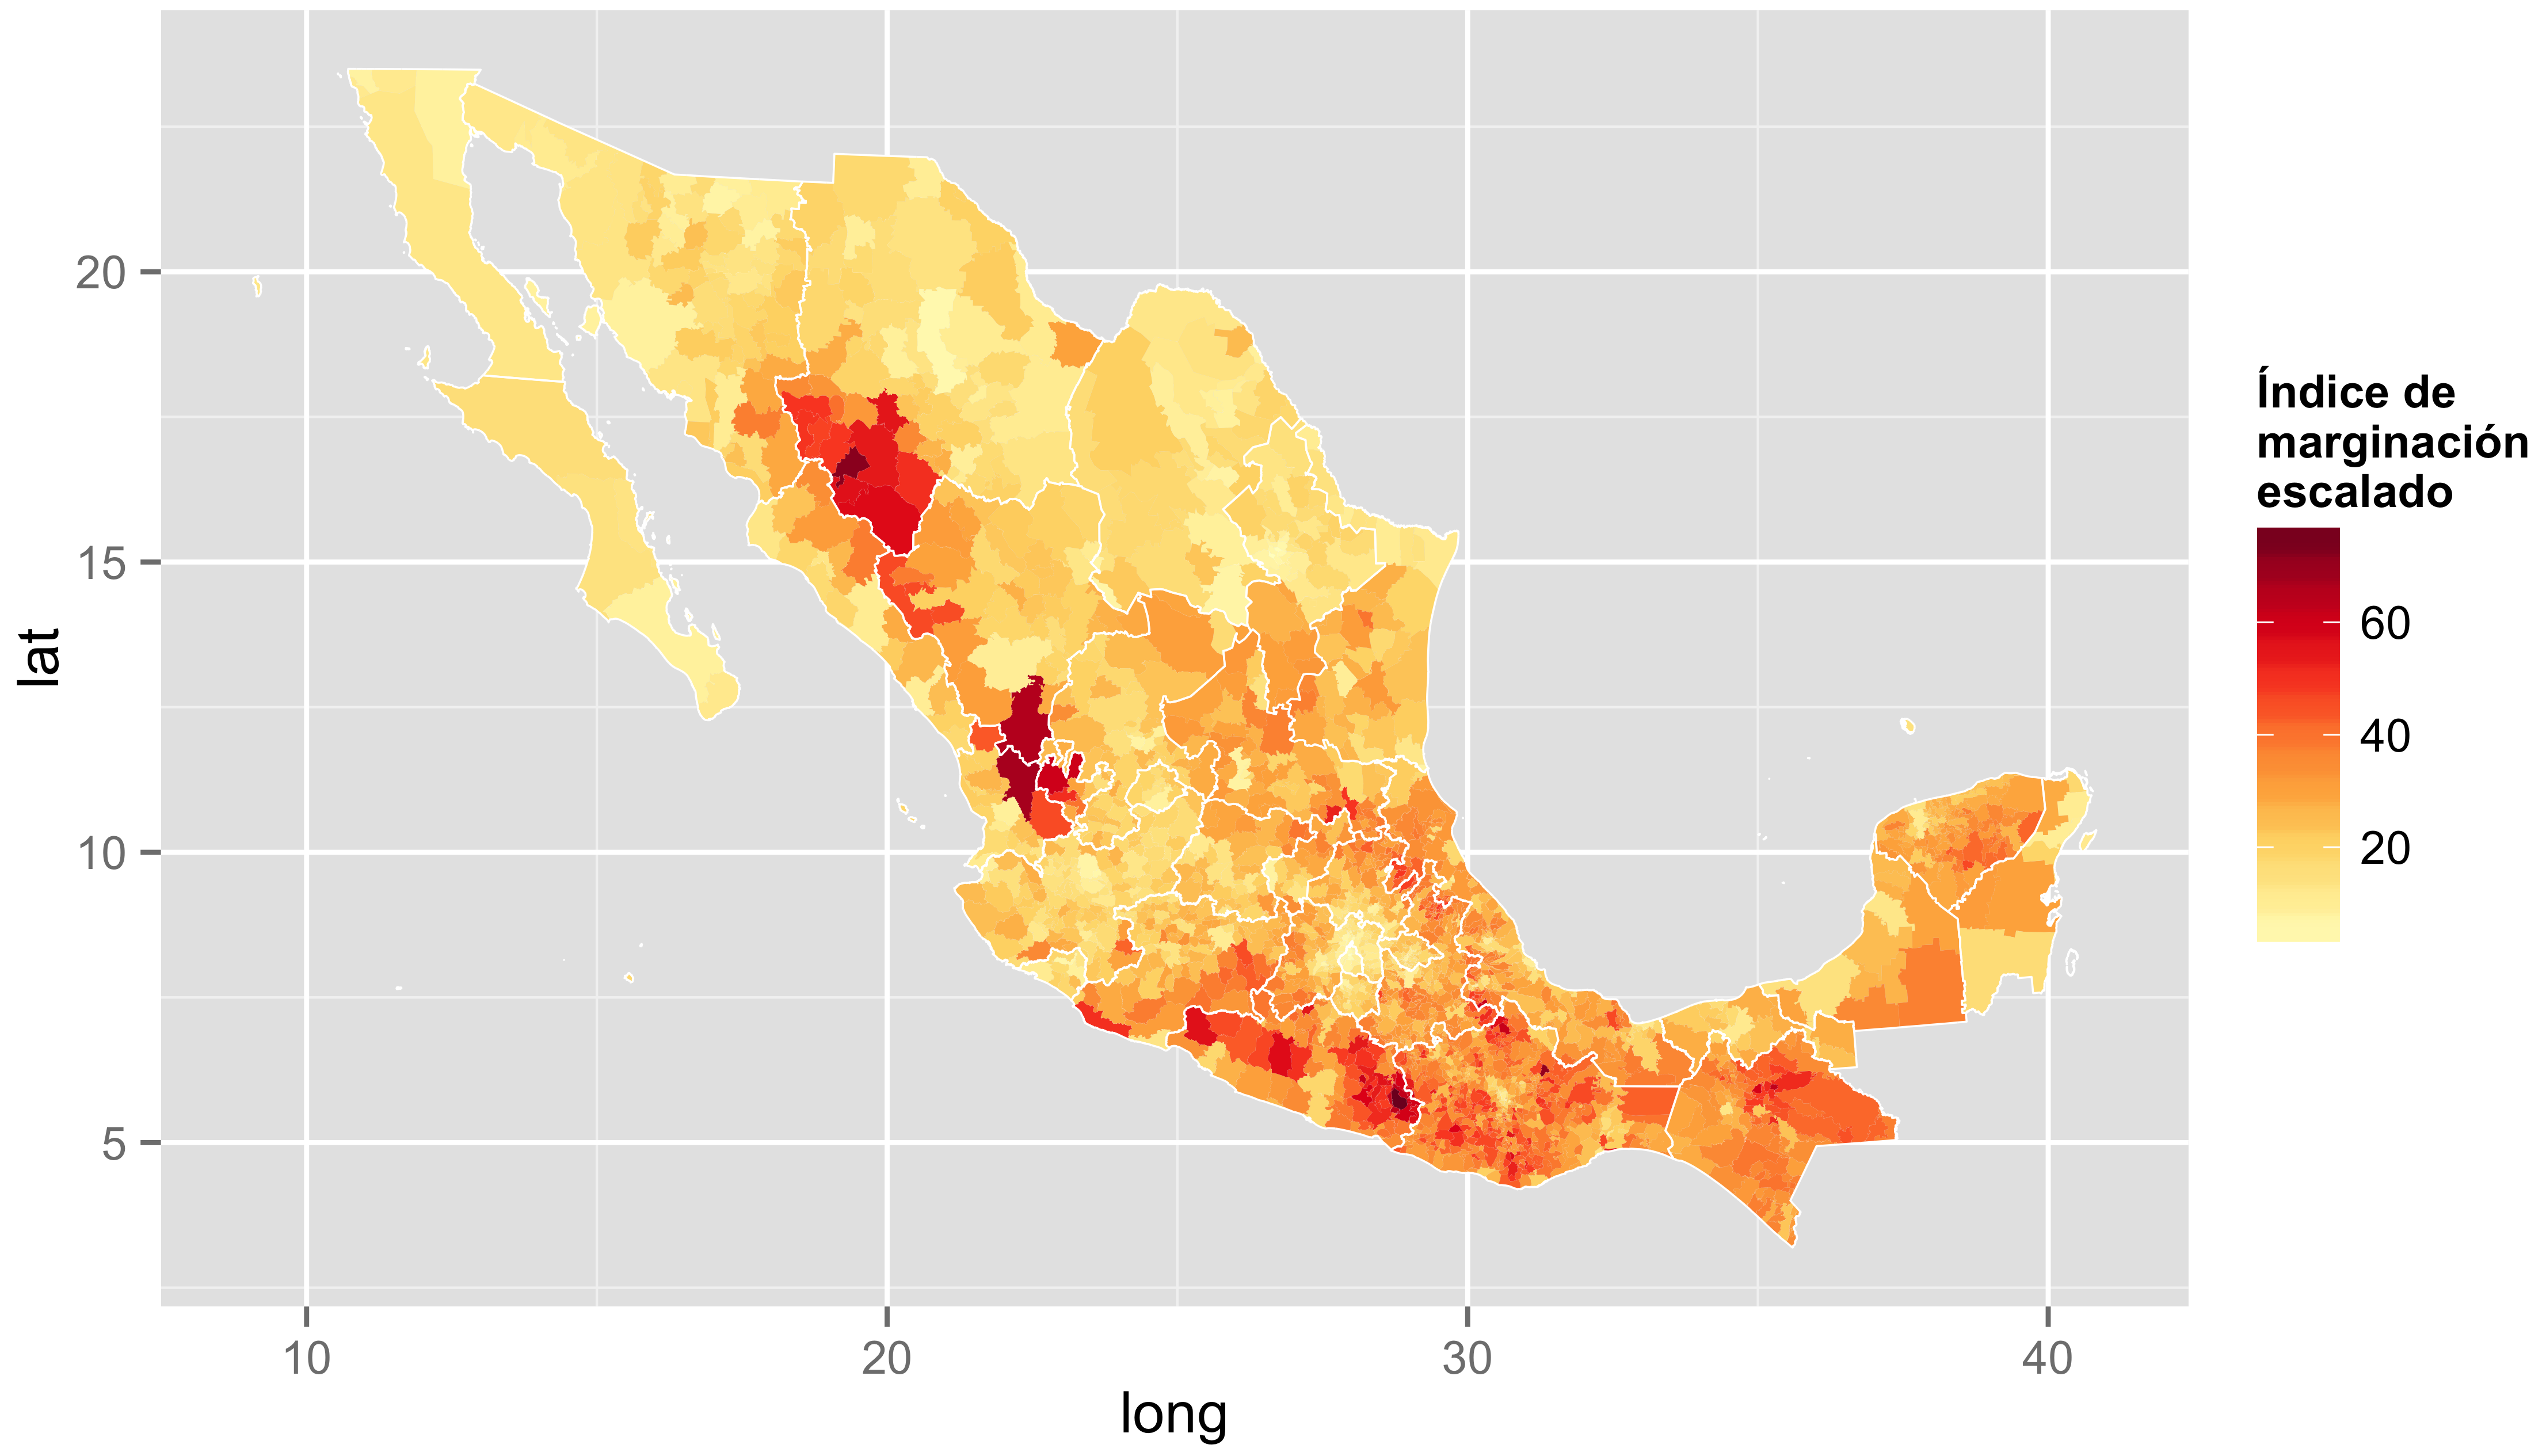
\includegraphics[scale=.20]{./maps/mapmarg.png} \\
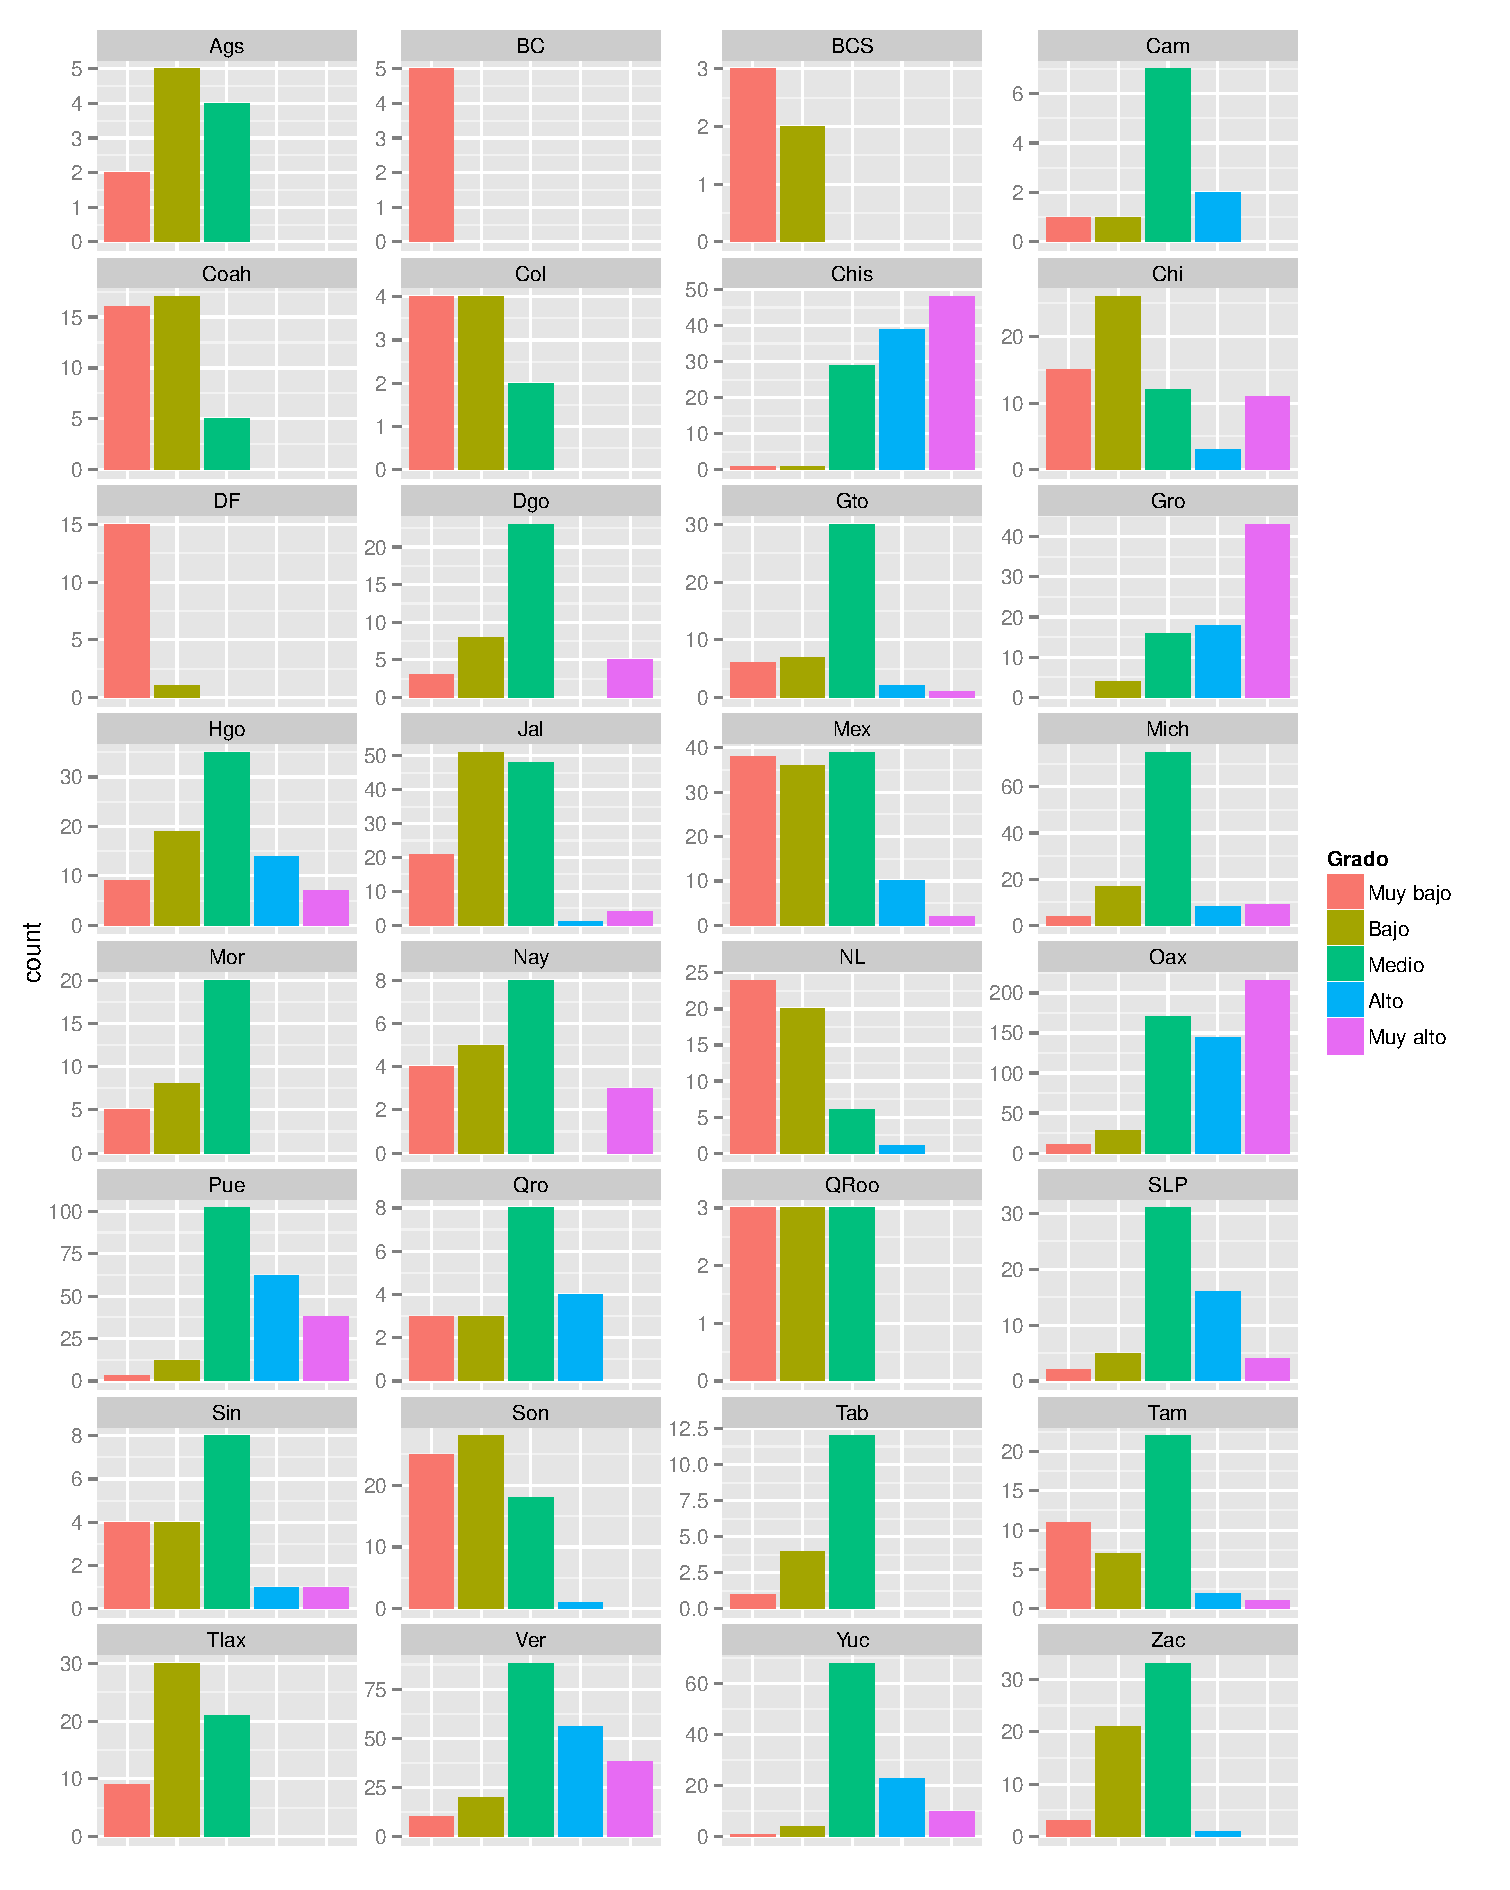
\includegraphics[width=\textwidth]{./plots/gmarg_plot.pdf} \\
\caption{Conteo grados de marginación.}
\label{obj:gradosmarg}  
\end{figure}

Observamos que Guerrero, Chiapas y Oaxaca destacan por tener gran proporción de municipios con grados de marginación ``Alto'' y ``Muy Alto'', corroborando lo que habíamos notado anteriormente con base en el mapa~\ref{obj:mapmarg}.

\section{Pruebas de autocorrelación espacial para índice de marginación}
Habiendo observado los datos, se harán las pruebas de autocorrelación espacial de Moran y de Geary para el índice de marginación.

Los pesos $w_{ij}$ a utilizar son los pesos binarios estandarizados por fila.
\subsection{Índice $\mathcal{I}$}
El valor del estimador $\mathcal{I}$, tiene el valor de 
\begin{equation}
\Hat{\mathcal{I}} = 0.703 .
\end{equation}

Sea $\mathcal{I}_0$ el valor esperado de $\mathcal{I}$ bajo la hipótesis nula, como esperamos autocorrelación espacial positiva para el índice de marginación, usamos la hipótesis alternativa $H_0: \mathcal{I}>\mathcal{I}_0$.


Utilizando los distintos supuestos, obtenemos los siguientes resultados.
\subsubsection{Bajo el supuesto de normalidad}
Se obtuvieron los siguientes resultados
\begin{align*}
\EN [ \widehat{\mathcal{I}}] =& -0.000407332,  \\ 
\VarN(\widehat{\mathcal{I}}) =& 0.000148633, \\
z =& 57.6945, \\
\mbox{valor-p} <& 2.2 \times 10^{-16}.
\end{align*}

El valor del estadístico $z$ está muy lejos de la región de no rechazo de $H_0$, es claro que rechazamos la hipótesis nula de no autocorrelación, y por lo tanto, $\Hat{\mathcal{I}}$ es significativamente mayor que $\mathcal{I}_0$.

\subsubsection{Bajo el supuesto de aleatorización}
Bajo el supuesto de aleatorización, se obtuvieron resultados bastante similares

\begin{align*}
\widehat{\ER [ \widehat{\mathcal{I}}]} =& -0.0004073320,  \\ 
\widehat{\VarN(\widehat{\mathcal{I}})} =& 0.0001486393, \\
z =& 57.6933, \\
\mbox{valor-p} <& 2.2 \times 10^{-16}.
\end{align*}

El valor del estadístico $z$ bajo este supuesto es practicamente el mismo que bajo el supuesto de normalidad, de la misma manera rechazamos la hipótesis nula de no autocorrelación espacial.
\subsubsection{Simulaciones de Monte Carlo}
Como el supuesto de normalidad es sensible es sensible a varios factores, es recomendable hacer simulaciones de Monte Carlo (vease \ref{sec:montecarlo}) para muestrear de la distribución de $\mathcal{I}$ .

Usando $n_{sim}=9999$, se obtuvieron los siguientes resultados
\begin{align*}
\mbox{orden observado} =& 10000,\\
\mbox{valor-p} =& 1\times 10^{-4}.
\end{align*}

Es decir, las  $9999$ observaciones del muestreo cayeron por debajo de $\Hat{\mathcal{I}}$. Por lo tanto, esta prueba también nos indica claramente autocorrelación espacial positiva.

En la gráfica \ref{obj:morandensity} podemos ver la densidad obtenida a partir de la muestra de Monte Carlo. 

\begin{figure}[!ht]
\centering
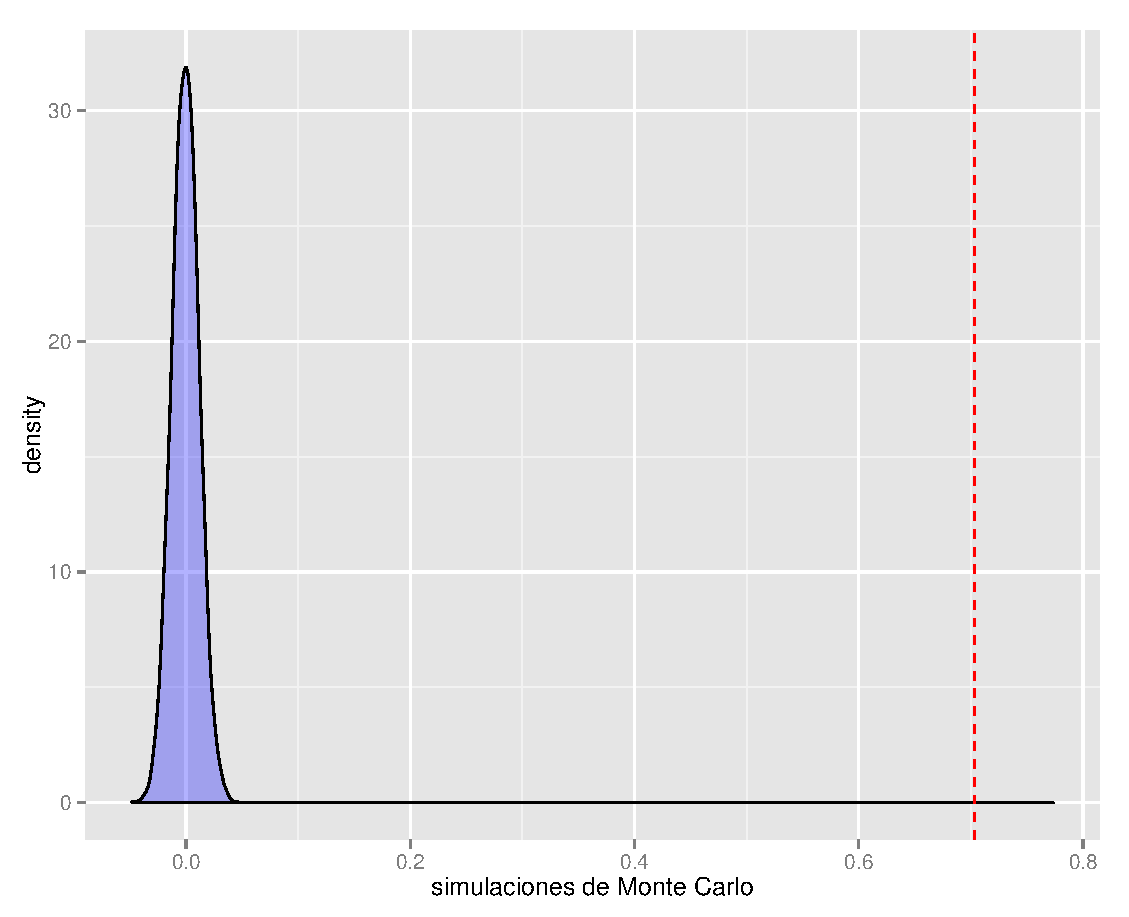
\includegraphics[width=.6\textwidth]{./plots/moran_density.pdf} \\
\caption{Densidad de la muestra de Monte Carlo de $\mathcal{I}$. La línea punteada índica donde se encuentra $\Hat{\mathcal{I}}$.}
\label{obj:morandensity}  
\end{figure}

\begin{itemize}
\item Viendo la forma de la densidad, el supuesto de normalidad parece muy razonable.  
\item Se observa como $\Hat{\mathcal{I}}$ cae muy lejos de la densidad de $I$ bajo el supuesto de no autocorrelación espacial. 
\end{itemize}



\subsection{Índice $\mathcal{C}$}
El valor del estimador $\Hat{\mathcal{C}}$, tiene el valor de 
\begin{equation}
\Hat{\mathcal{C}} = 0.2943260693 .
\end{equation}

Sea, $\mathcal{C}_0$ el valor esperado de $\mathcal{C}$ bajo la hipótesis nula, como esperamos autocorrelación espacial positiva para el índice de marginación, usamos la hipótesis alternativa $\mathcal{C}<\mathcal{C}_0$, sin embargo, como construimos el estadístico $z$ en la ecuación \ref{eq:zgeary}, esperamos que el estadístico $z$ observado sea significativamente mayor a $z$ bajo la hipótesis nula.


Así, utilizando los distintos supuestos, obtenemos los siguientes resultados.

\subsubsection{Bajo supuesto de normalidad}
Se obtuvieron los siguientes resultados
\begin{align*}
\EN [\widehat{\mathcal{C}}] =& 1,  \\ 
\VarN(\widehat{\mathcal{C}}) =& 0.0001911584, \\
z =& 51.0396, \\
\mbox{valor-p} <& 2.2 \times 10^{-16}.
\end{align*}

El valor del estadístico $z$ está muy lejos de la región de no rechazo de $H_0$, es claro que rechazamos la hipótesis nula de no autocorrelación, y por lo tanto, $\Hat{\mathcal{C}}$ es significativamente menor que $\mathcal{C}_0$.


\subsubsection{Bajo supuesto de aleatorización}

Bajo el supuesto de aleatorización, se obtuvieron resultados bastante similares

\begin{align*}
\widehat{\EN [\widehat{\mathcal{C}}]} =& 1,  \\ 
\widehat{\VarN(\widehat{\mathcal{C}})} =& 0.0001889559,  \\
z =& 51.3362, \\
\mbox{valor-p} <& 2.2 \times 10^{-16}.
\end{align*}

El valor del estadístico $z$ bajo este supuesto es practicamente el mismo que bajo el supuesto de normalidad, de la misma manera rechazamos la hipótesis nula de no autocorrelación espacial.
\subsubsection{Simulaciones de Monte Carlo}
Al igual que hicimos con el coeficiente de Morano, ahora muestreamos  de la distribución de $\mathcal{C}$. 

Usando $n_{sim}=9999$, se obtuvieron los siguientes resultados
\begin{align*}
\mbox{orden observado} &= 1,\\
\mbox{valor-p} &= 1\times 10^{-4}.
\end{align*}

Es decir, las  $9999$ observaciones del muestreo cayeron por encima de $\Hat{\mathcal{C}}$. Por lo tanto, esta prueba también nos indica claramente autocorrelación espacial positiva.

En la gráfica \ref{obj:gearydensity} podemos ver la densidad obtenida a partir de la muestra de Monte Carlo. 

\begin{figure}[!ht]
\centering
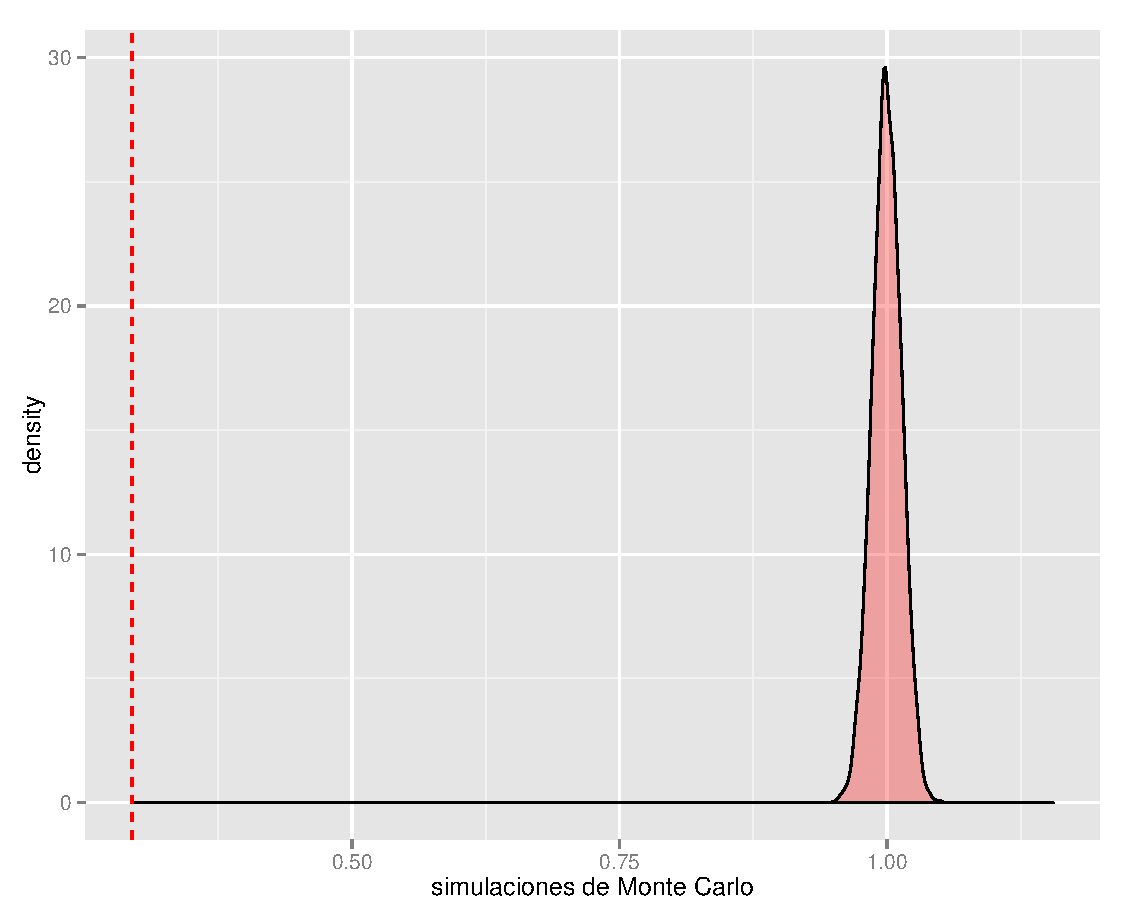
\includegraphics[width=.6\textwidth]{./plots/geary_density.pdf} \\
\caption{Densidad de la muestra de Monte Carlo de $\mathcal{C}$. La línea punteada índica donde se encuentra $\Hat{\mathcal{C}}$.}
\label{obj:gearydensity}  
\end{figure}

\begin{itemize}
\item Viendo la forma de la densidad, el supuesto de normalidad parece muy razonable.  
\item Se observa como $\Hat{\mathcal{C}}$ cae muy por debajo de la densidad de $C$ bajo el supuesto de no autocorrelación espacial. 
\end{itemize}




\section{Análisis de conglomerados}
Ahora, procedemos a agrupar los municipios por similitud. Para comparar los municipios, utilizaremos las variables que definen las cinco dimensiones de marginación propuesto por \citet{conapo04}: analf, sprim, sdren, selec, sagua, hacina, pisot, l5kha y bingreso.

Se utilizará el algoritmo de $k$-medias esférico que utiliza como medida de disimilitud entre observaciones, la disimilitud de cosenos.

\subsection{Determinación de $K^*$ utilizando el estadístico Gap}

Empezamos escogiendo el número de grupos $K^*$ a través del estadístico Gap. Escogiendo el número máximo de valores K a probar $M=10$, y $B=100$ para el tamaño de la muestra de Monte Carlo, podemos ver los resultados en la tabla~\ref{tab:gaptable}.

\begin{table}[ht]
\centering
\begin{tabular}{rrrrr}
  \hline
 & $\log{W_K}$ & $E^*\lbrace \log{W_K} \rbrace $ & $\mbox{Gap}_K$ & $s_K$ \\ 
  \hline
  1 & 5.5489 & 6.1259 & 0.5770 & 0.00389 \\ 
  2 & 5.3049 & 5.9731 & 0.6682 & 0.00318 \\ 
  3 & 5.1981 & 5.9205 & 0.7225 & 0.00298 \\ 
  4 & 5.1272 & 5.8754 & 0.7481 & 0.00305 \\ 
  5 & 5.0644 & 5.8431 & 0.7787 & 0.00283 \\ 
  6 & 5.0364 & 5.8140 & 0.7776 & 0.00307 \\ 
  7 & 5.0024 & 5.7921 & 0.7897 & 0.00307 \\ 
  8 & 4.9711 & 5.7707 & 0.7995 & 0.00290 \\ 
  9 & 4.9501 & 5.7543 & 0.8042 & 0.00293 \\ 
  10 & 4.9317 & 5.7392 & 0.8075 & 0.00300 \\ 
   \hline
\end{tabular}
\caption{Valor de Gap para $K$, $K=1,2, \dots, 10$. \label{tab:gaptable}}
\end{table}

Observando la gráfica \ref{obj:gapplot} y utilizando el criterio de \citet{hastie09} (véase la ecuación \ref{tibshiranicriteria}) encontramos que $K^*=5$.


\begin{figure}[!ht]
  \centering
  \caption{Gráfica del estadístico Gap. \label{obj:gapplot} }
  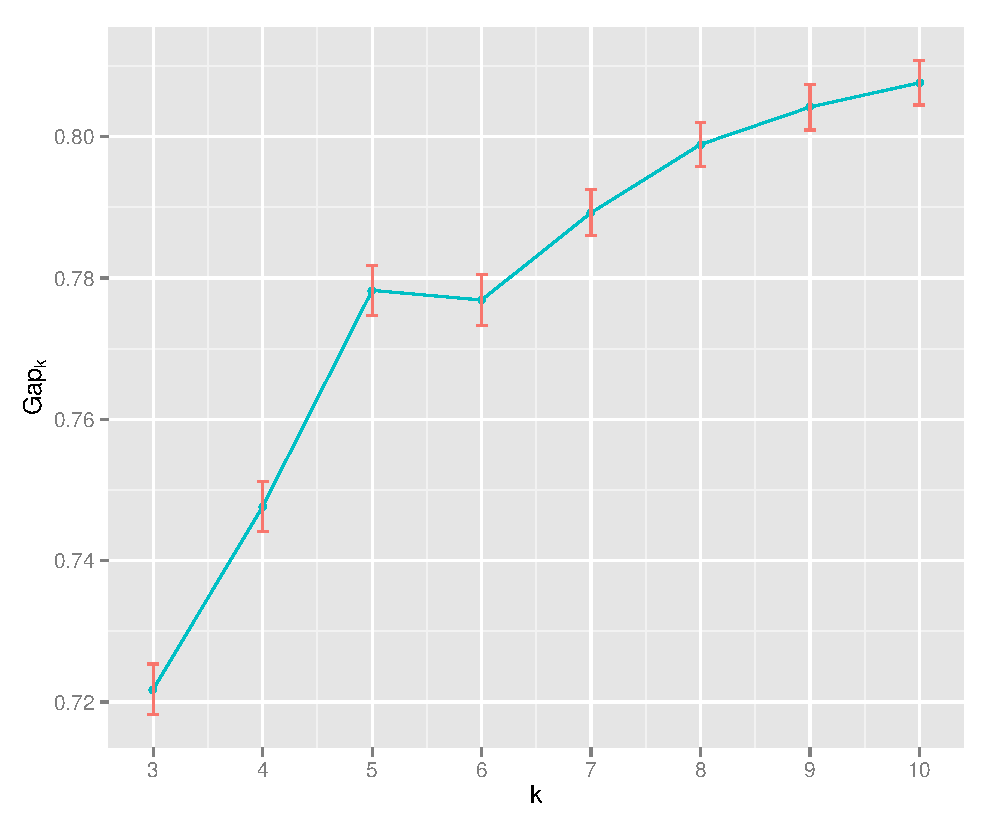
\includegraphics[width=.7\textwidth]{./plots/gap_plot.pdf}
\end{figure}

\subsection{Resultado de $K$-medias esféricas}
Habiendo obtenido que $K^*=5$, corremos el algoritmo de $k$-medias esféricas sobre las variables mencionadas anteriormente.

Podemos ver la distribución de  los 5 grupos en la tabla \ref{tabla5g} y en la gráfica \ref{obj:graf5g}.

\begin{table}[!ht]
\centering
\begin{tabular}{rrr}
  \hline
    & conteo & \% \\ 
  \hline
  1 & 490 & 20\% \\ 
  2 & 455 & 19\% \\ 
  3 & 808 & 33\% \\ 
  4 & 274 & 11\% \\ 
  5 & 429 & 17\% \\ 
   \hline
\end{tabular}
\caption{Tabla del tamaño de los 5 Grupos. \label{tabla5g}}
\end{table}

\begin{figure}[!ht]
  \centering
  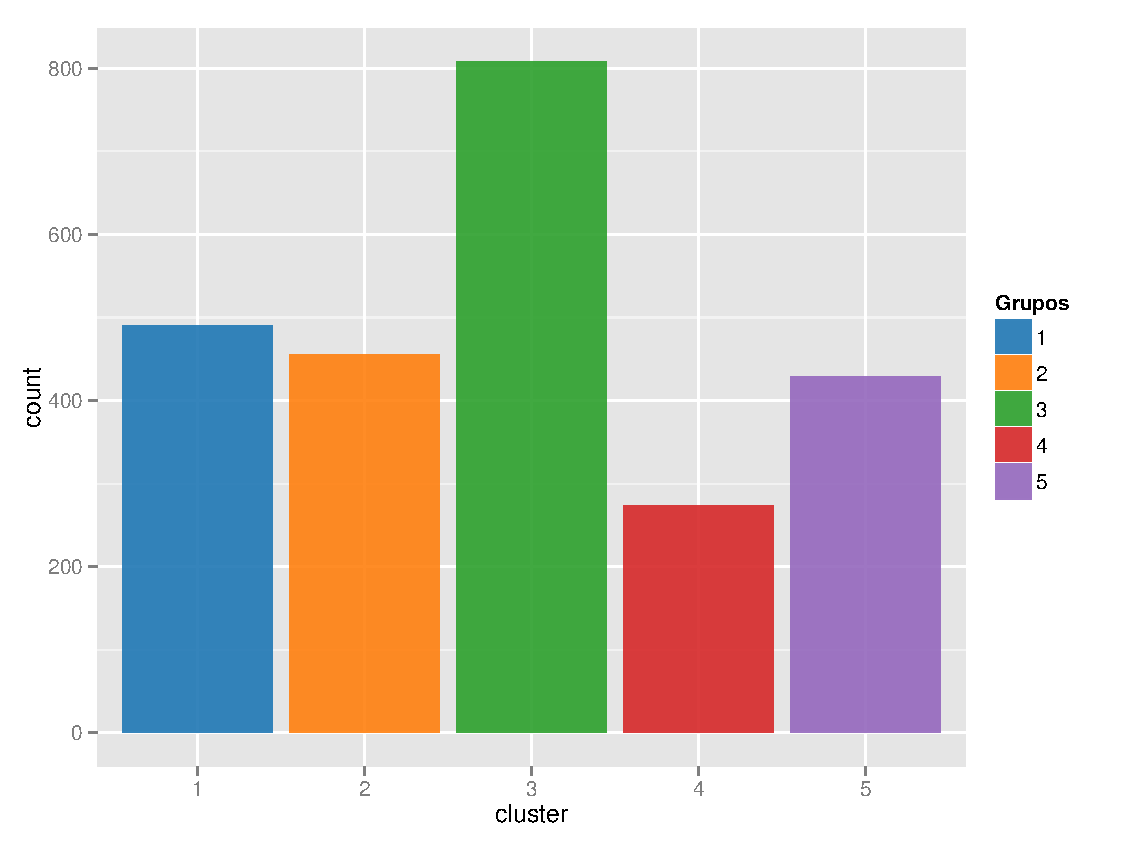
\includegraphics[width=.7\textwidth]{./plots/clustering_plot.pdf}
  \caption{Distribución de los grupos. \label{obj:graf5g} }
\end{figure}

Vemos que en el grupo 3 es donde cayeron más observaciones (33\%), mientras que en el 4 cayó el menor número de observaciones (11\%). Los demás grupos tienen una distribución similar.

Ahora, en la tabla \ref{tab:centroides} vemos los centroides de cada grupo. Éstos nos dan una caracterización de cada uno de los grupos.

\begin{table}
\centering
\begin{tabular}{rrrrrrrrrr}
  \hline
 & analf & sprim & sdren & selec & sagua & hacina & pisot & pl5khab & bingreso\\ 
  \hline
  1 & 0.07 & 0.24 & 0.05 & 0.02 & 0.05 & 0.30 & 0.05 & \textbf{0.81} & 0.44 \\ 
  2 & \textbf{0.14} & 0.29 & \textbf{0.08} & \textbf{0.06} & \textbf{0.32} & 0.37 & \textbf{0.15} & 0.60 & 0.51 \\ 
  3 & 0.13 & 0.30 & 0.05 & 0.03 & 0.07 & 0.37 & 0.12 & 0.66 & 0.54 \\ 
  4 & 0.09 & 0.30 & 0.03 & 0.02 & 0.09 & \textbf{0.67 }& 0.08 & 0.12 & \textbf{0.65} \\ 
  5 & 0.12 & \textbf{0.34} & 0.05 & 0.02 & 0.09 & 0.53 & 0.10 & 0.43 & 0.62 \\ 
   \hline
\end{tabular}
\caption{Centroides de los 5 conglomerados. \label{tab:centroides}}
\end{table}



En el mapa coroplético \ref{mapgroupsmarg} se colorea cada municipio de acuerdo al grupo en el que cayó.

\begin{landscape}
  \begin{figure}[!ht]
    \centering
    \caption[skip=0pt]{Mapa de México con los municipios coloreados por grupo. \label{mapgroupsmarg} }
    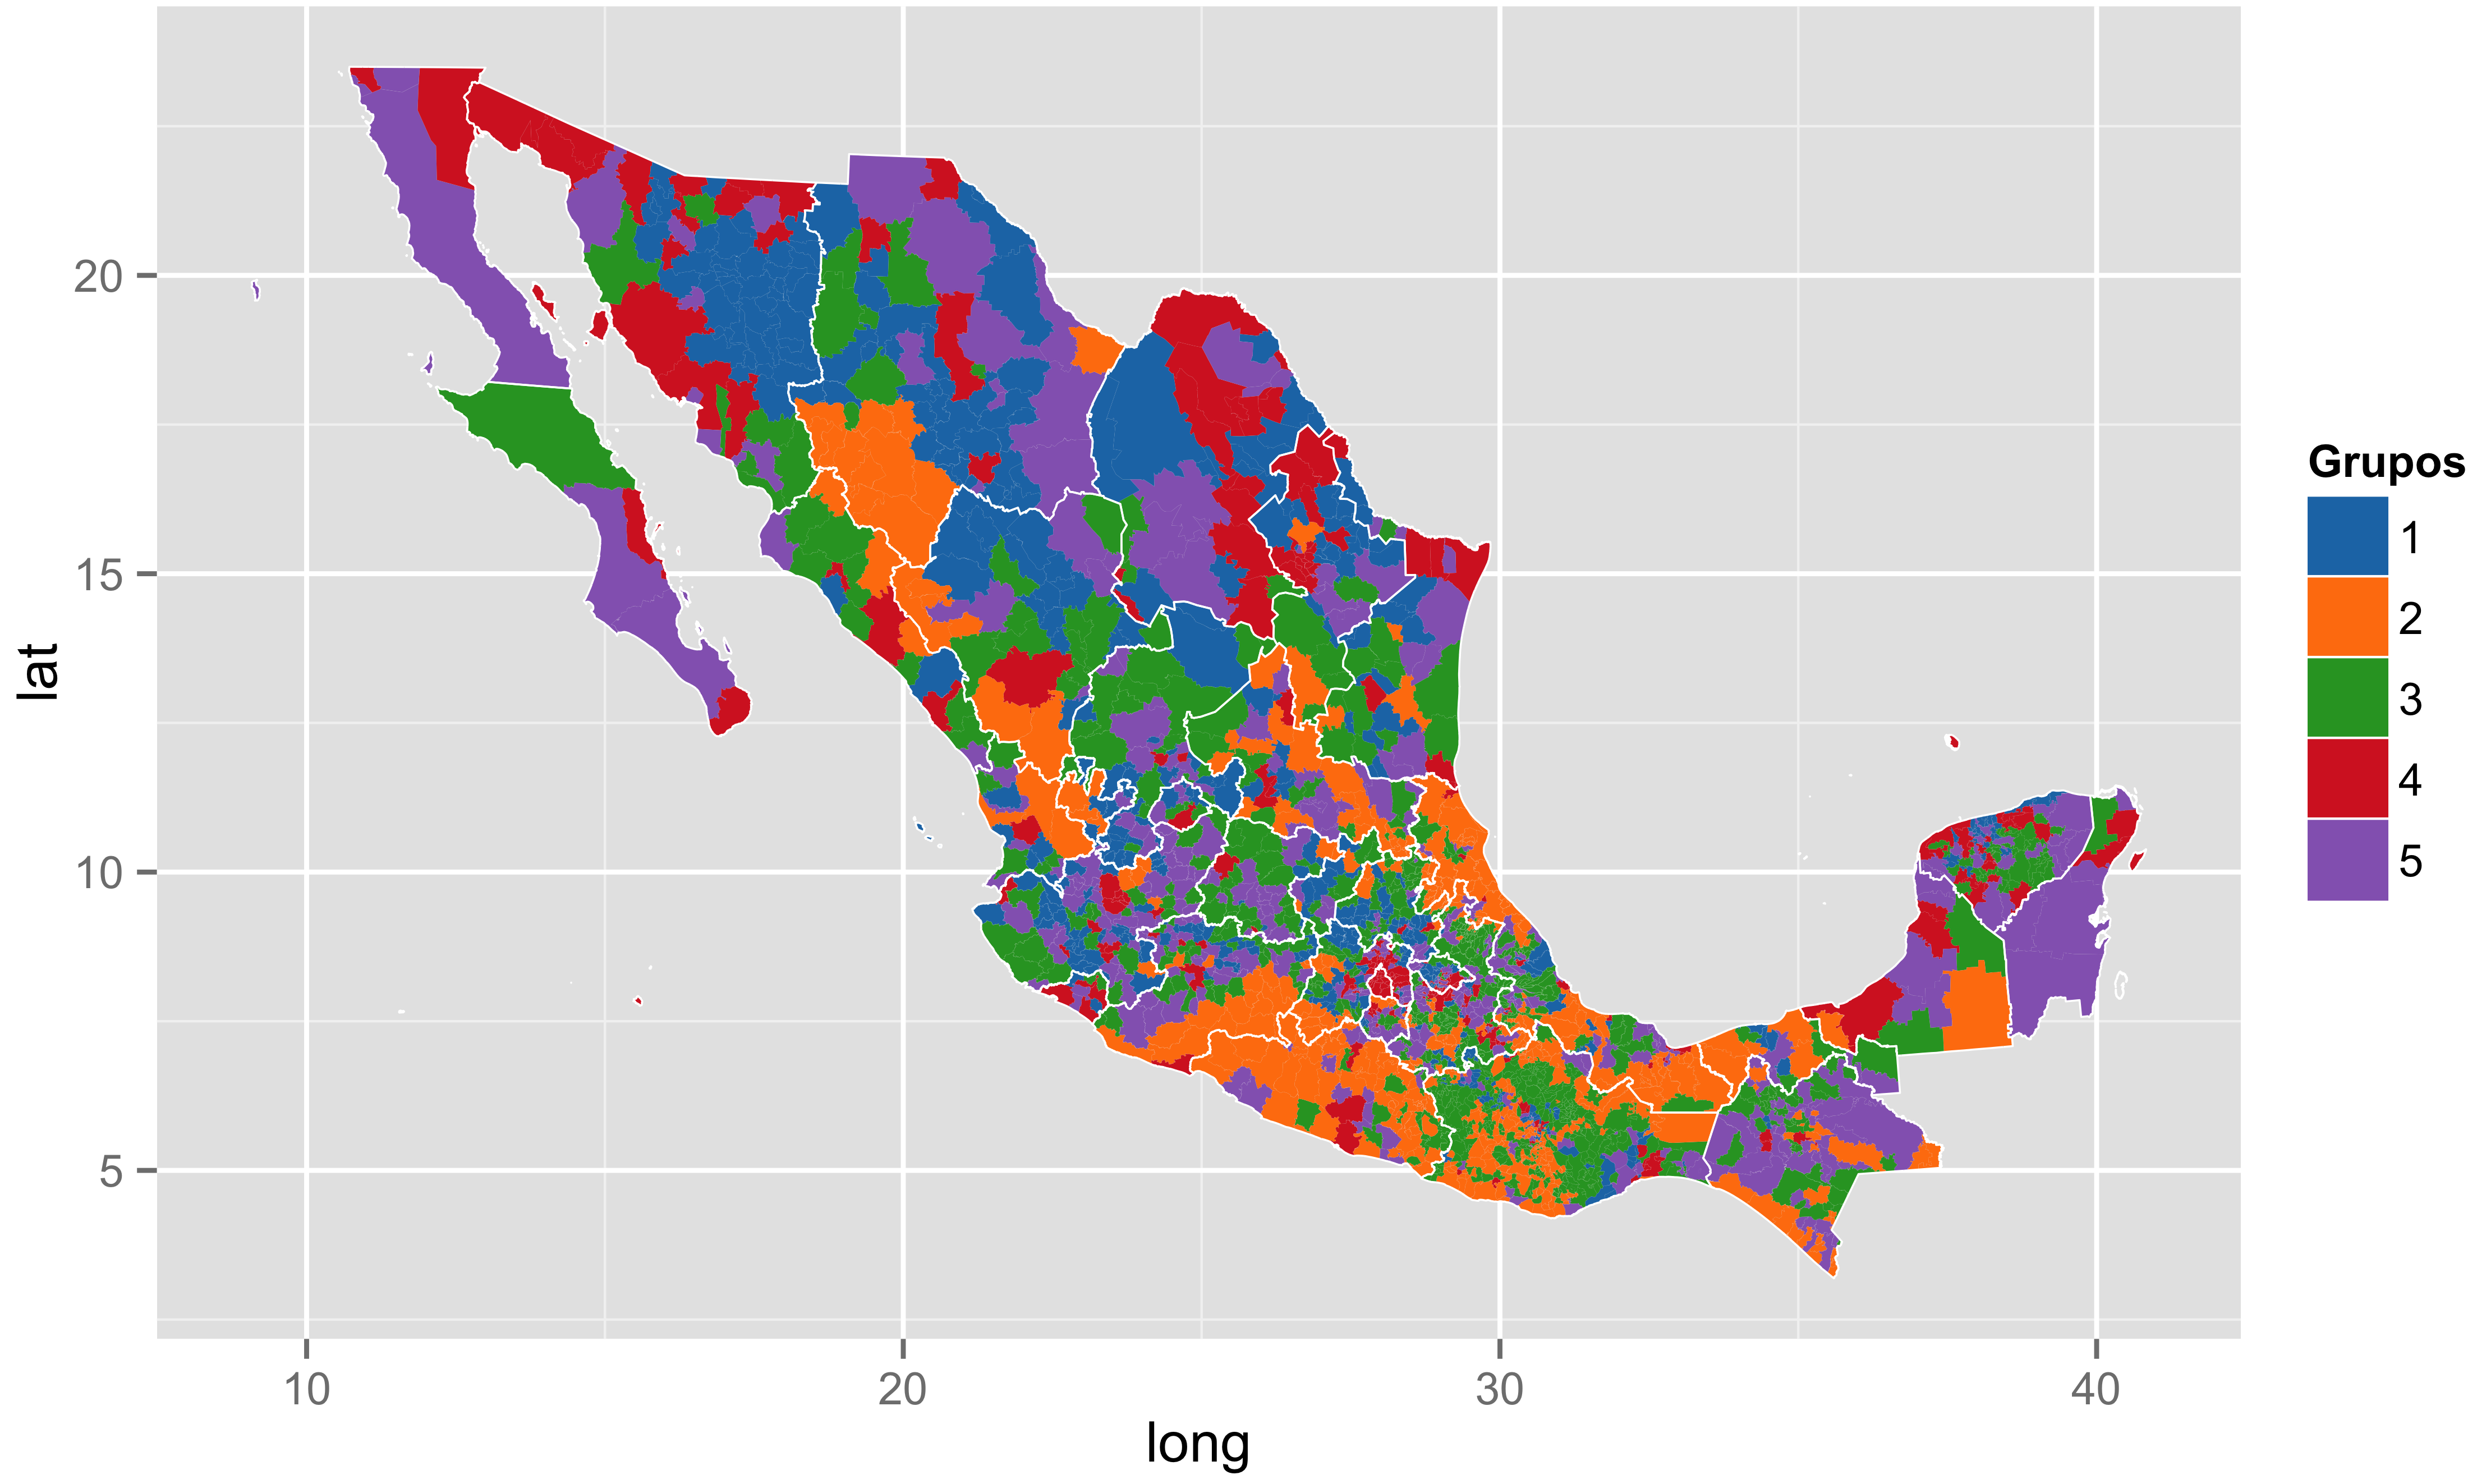
\includegraphics[width=1.4\textheight]{./maps/map5g.png}
  \end{figure}
\end{landscape}

En la gráfica \ref{obj:boxplotgroup} vemos la distribución por grupo de las 9 variables utilizadas en el algoritmo de conglomerados esféricos y en la gráfica \ref{obj:gradomarggrupos} vemos la distribución de los grupos de marginación por grupo.

\begin{figure}[!ht]
  \centering
  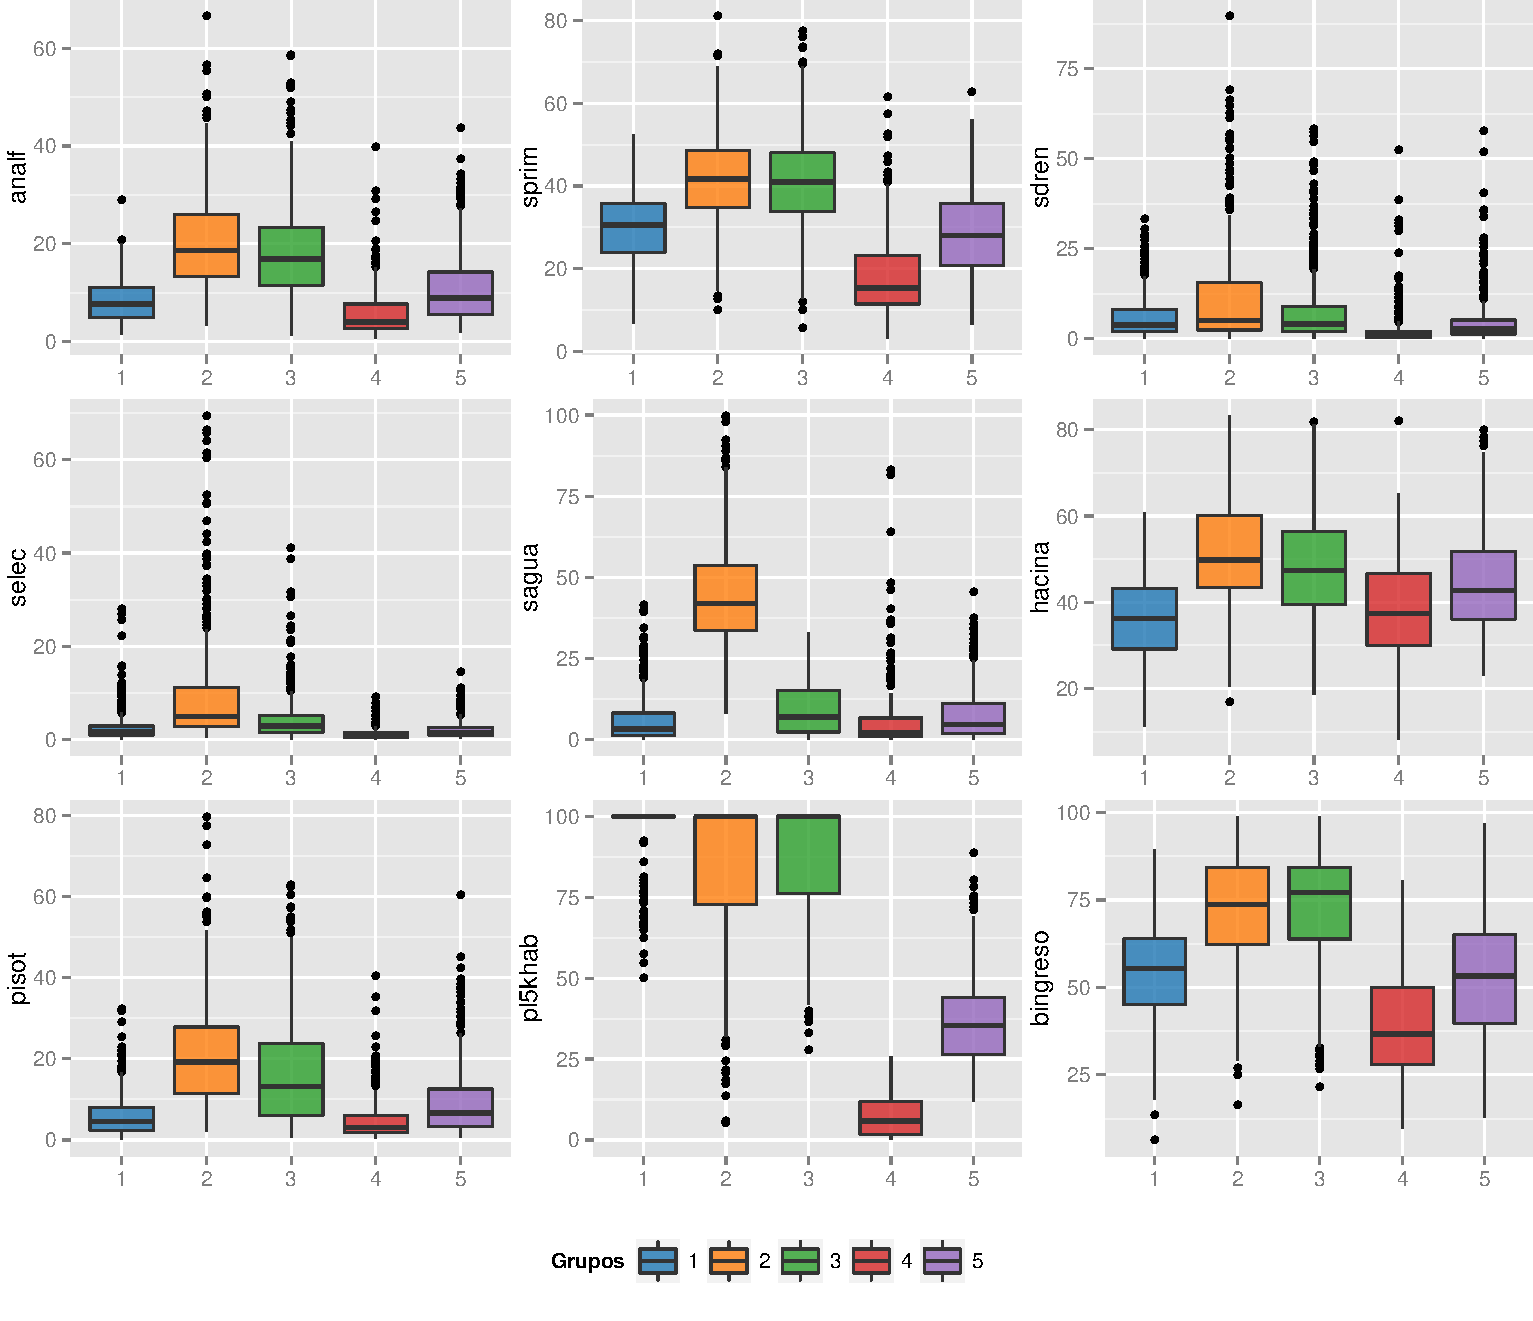
\includegraphics[width=\textwidth]{./plots/boxplot_bygroup.pdf}
  \caption{Distribución de variables de marginación por grupo. \label{obj:boxplotgroup} }
\end{figure}



\begin{figure}[!ht]
  \centering
  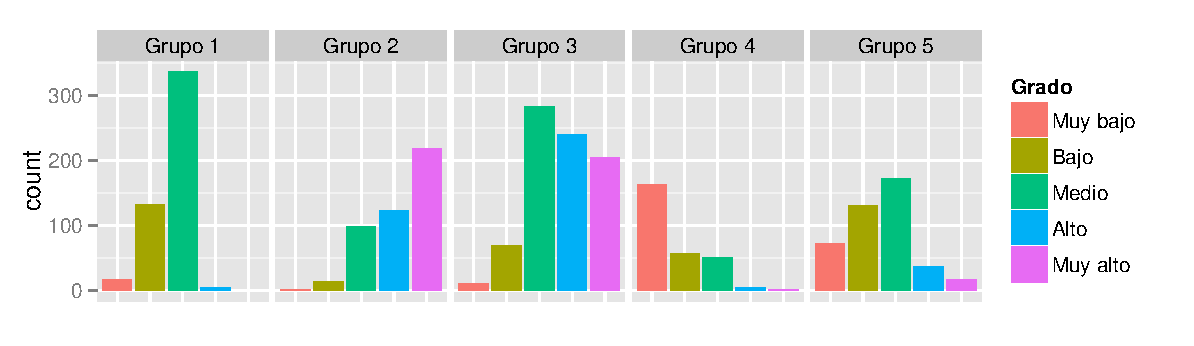
\includegraphics[width=\textwidth]{./plots/gmarg_group.pdf}
  \caption{Grado de marginación por grupo. \label{obj:gradomarggrupos} }
\end{figure}

A partir de la tabla \ref{tab:centroides}, las gráficas \ref{obj:gradomarggrupos} y \ref{obj:boxplotgroup} y observando el mapa \ref{mapgroupsmarg} podemos recalcar lo más característico de cada uno de los cinco grupos.

\begin{itemize}
\item \textbf{Grupo 1}: Se caracteriza por tener municipios con un alto porcentaje de población en localidades con menos de 5,000 habitantes y poco marginados. De hecho podemos observar en la gráfica \ref{obj:gradomarggrupos} que principalmente hay municipios con grado de marginación ``Medio'' y ``Medio Bajo''. Los municipios más cercanos al centroide los podemos ver en la tabla \ref{tab:grupo1}.

\begin{table}[!ht]
\centering
\begin{tabular}{rllrlr}
  \hline
 & nom\_mun & estado & imarges & gmarg & disim \\ 
  \hline
1 & Viesca & Coah & 21.74 & Medio & 0.00153 \\ 
  2 & San Gabriel & Jal & 22.51 & Medio & 0.00154 \\ 
  3 & Villa de la Paz & SLP & 20.62 & Medio & 0.00160 \\ 
  4 & Santa María del Oro & Nay & 23.24 & Medio & 0.00176 \\ 
  5 & Nazas & Dgo & 22.21 & Medio & 0.00206 \\ 
   \hline
\end{tabular}
\caption{Municipios más representativos del grupo 1. La columna disim corresponde a la disimilitud de cosenos entre la observación $i$ y el centroide del grupo 1. \label{tab:grupo1}}
\end{table}

\item \textbf{Grupo 2}: En este grupo se encuentran los municipios más marginados mencionados en la tabla \ref{tab:masmarg}. El grado de marginación de dichos municipios es ``Muy Alto'', ``Alto'' o ``Medio'' (ver gráfica \ref{obj:gradomarggrupos}). 
Se caracteriza por tener porcentajes altos en: población analfabeta y ocupantes en viviendas sin drenaje ni escusado, sin energía eléctrica, con piso de tierra y sin agua entubada. De hecho, es el grupo que tiene mayor porcentaje de viviendas sin agua entubada, siendo la principal característica que lo diferencia del grupo 3. Podemos ver en la tabla \ref{tab:grupo2} los municipios más representativos.

\begin{table}[ht]
\centering
\begin{tabular}{rllrlr}
  \hline
 & nom\_mun & estado & imarges & gmarg & disim \\ 
  \hline
1 & Xochiatipan & Hgo & 45.17 & Muy alto & 0.00216 \\ 
  2 & Coxquihui & Ver & 43.21 & Muy alto & 0.00356 \\ 
  3 & Playa Vicente & Ver & 32.72 & Alto & 0.00357 \\ 
  4 & Zozocolco de Hidalgo & Ver & 47.71 & Muy alto & 0.00372 \\ 
  5 & San Pedro Ixcatlán & Oax & 42.32 & Muy alto & 0.00416 \\ 
   \hline
\end{tabular}
\caption{Municipios más representativos del grupo 2. La columna disim corresponde a la disimilitud de cosenos entre la observación $i$ y el centroide del grupo 2. \label{tab:grupo2}}
\end{table}

\item \textbf{Grupo 3}: Como en el grupo 1, los municipios del grupo 3 tienen alto porcentaje de localidades pequeñas (menos de $5,000$ habitantes), pero los municipios tienen grado de marginación  ``Muy Alto'', ``Alto'' o ``Medio''. Además los municipios en este grupo, tienen porcetajes altos de población ocupada con ingreso de hasta 2 salarios mínimos. En la tabla \ref{tab:grupo3} podemos ver las observaciones más representativas.

\begin{table}[ht]
\centering
\begin{tabular}{rllrlr}
  \hline
 & nom\_mun & estado & imarges & gmarg & disim \\ 
  \hline
1 & Amatenango de la Frontera & Chis & 37.35 & Alto & 0.00102 \\ 
  2 & Coetzala & Ver & 35.01 & Alto & 0.00119 \\ 
  3 & Mártires de Tacubaya & Oax & 34.38 & Alto & 0.00160 \\ 
  4 & Totutla & Ver & 33.94 & Alto & 0.00187 \\ 
  5 & Juan N. Méndez & Pue & 36.20 & Alto & 0.00205 \\ 
   \hline
\end{tabular}
\caption{Municipios más representativos del grupo 3. La columna disim corresponde a la disimilitud de cosenos entre la observación $i$ y el centroide del grupo 3. \label{tab:grupo3}}
\end{table}

Es el grupo más grande con 808 municipios, representando un 33\% del total.

\item \textbf{Grupo 4}: En este grupo podemos encontrar muchos municipios con baja marginación. Es el grupo más pequeño con tan solo el 11\% de las observaciones. Todas las delegaciones del Distrito Federal y los principales municipios de la Ciudad de Monterrey, en Nuevo León, están en este grupo. En este grupo, los municipios tienen un porcentaje relativamente bajo de viviendas con algún nivel de hacinamiento, bajo porcentaje de población ocupada con ingreso de hasta 2 salarios mínimos y bajo porcentaje de población de 15 años o más sin primaria completa. Los cinco municipios más representativos los podemos ver en la tabla  \ref{tab:grupo4}.


\begin{table}[!ht]
\centering
\begin{tabular}{rllrlr}
  \hline
 & nom\_mun & estado & imarges & gmarg & disim \\ 
  \hline
1 & Jiutepec & Mor & 8.60 & Muy bajo & 0.00143 \\ 
  2 & Cuernavaca & Mor & 7.26 & Muy bajo & 0.00187 \\ 
  3 & Coatzacoalcos & Ver & 11.22 & Muy bajo & 0.00188 \\ 
  4 & Matamoros & Tam & 10.82 & Muy bajo & 0.00382 \\ 
  5 & Río Bravo & Tam & 13.51 & Muy bajo & 0.00392 \\ 
   \hline
\end{tabular}
\caption{Municipios más representativos del grupo 4. La columna disim corresponde a la disimilitud de cosenos entre la observación $i$ y el centroide del grupo 4. \label{tab:grupo4}}
\end{table}

Podemos encontrar también algunos lugares turísticos como San Cristóbal de las Casas, Acapulco, Benito Juárez en Quintana Roo (aquí se encuentra Cancún), Los Cabos, Puerto Vallarta, Veracruz, etc.

\item \textbf{Grupo 5}: Este grupo es muy parecido al grupo 1, pero los municipios dentro del grupo 5 tienen mayor porcentaje de poblaciones con más de $5,000$ habitantes, es decir, tienen poblaciones más grandes. Los cinco municipios más cerca del centroide 5 se encuentran en la tabla \ref{tab:grupo5}.

\begin{table}[ht]
\centering
\begin{tabular}{rllrlr}
  \hline
 & nom\_mun & estado & imarges & gmarg & disim \\ 
  \hline
1 & Villagrán & Gto & 16.83 & Bajo & 0.00137 \\ 
  2 & Cortazar & Gto & 16.38 & Bajo & 0.00186 \\ 
  3 & Angel Albino Corzo & Chis & 35.21 & Alto & 0.00232 \\ 
  4 & San Juan Bautista Tuxtepec & Oax & 19.51 & Bajo & 0.00277 \\ 
  5 & Celaya & Gto & 11.76 & Muy bajo & 0.00294 \\ 
   \hline
\end{tabular}
\caption{Municipios más representativos del grupo 5. La columna disim corresponde a la disimilitud de cosenos entre la observación $i$ y el centroide del grupo 5. \label{tab:grupo5}}
\end{table}

\end{itemize}

Otro punto que podemos destacar observando el mapa \ref{mapgroupsmarg}, es que existe cierta uniformidad espacial entre miembros del mismo grupo. Es decir, vemos que regiones que pertenecen al mismo grupo, comparten frontera. 

En la próxima sección se harán las pruebas de hipótesis para detectar la presencia de autocorrelación espacial positiva.


\section{Prueba de conteo de fronteras para conglomerados}

Sean $\Hat{N_{rs}}$ los conteo observado,  $N_{rs,0}$ los conteo esperado de fronteras del tipo $rs$, $r,s=1,2,3,4,5$.

Dado que no contamos con las $p_i$'s (probabilidad de que una región sea de tipo $i$) a priori, las estimamos a partir de los datos. Por lo tanto, en el siguiente análisis de autocorrelación espacial se utilizará el supuesto de muestreo sin reemplazo. También se utilizarán los pesos binarios estandarizados por renglón.

La tabla \ref{tab:conteobordes} donde se muestran los conteos de fronteras observados conteos esperados y las varianzas bajo muestreo sin reemplazo y el valor $z$ calculado. 
\begin{table}[ht]
\centering
\begin{tabular}{rrrrr}
  \hline
 & $\Hat{N_{rs}}$  & $N_{rs,0}$ & $\Var$ & $z$ \\ 
  \hline
  1:1 & 98.61 & 48.80 & 6.53 & 19.49 \\ 
  2:2 & 110.35 & 42.07 & 5.77 & 28.43 \\ 
  3:3 & 194.99 & 132.80 & 14.00 & 16.62 \\ 
  4:4 & 50.36 & 15.23 & 2.36 & 22.88 \\ 
  5:5 & 63.59 & 37.40 & 5.22 & 11.46 \\ 
  2:1 & 35.95 & 90.81 & 12.56 & -15.48 \\ 
  3:1 & 103.48 & 161.27 & 20.00 & -12.92 \\ 
  3:2 & 138.83 & 149.75 & 18.74 & -2.52 \\ 
  4:1 & 48.76 & 54.69 & 7.96 & -2.10 \\ 
  4:2 & 18.10 & 50.78 & 7.48 & -11.95 \\ 
  4:3 & 42.67 & 90.18 & 11.81 & -13.82 \\ 
  5:1 & 82.05 & 85.63 & 11.93 & -1.03 \\ 
  5:2 & 55.61 & 79.51 & 11.19 & -7.14 \\ 
  5:3 & 122.55 & 141.19 & 17.79 & -4.42 \\ 
  5:4 & 62.10 & 47.88 & 7.11 & 5.33 \\ 
  Jtot & 710.10 & 951.70 & 37.24 & -39.59 \\ 
   \hline
\end{tabular}
\caption{Conteo de fronteras.}
\label{tab:conteobordes}
\end{table}

Los conteos de fronteras entre municipios del mismo color son mucho mayores que lo esperado.Viendo el valor $z$ entre las fronteras del tipo $rr$, podemos resaltar que, para $1:1$, es el más alto con $28.43$; mientras que para $5:5$, es el más bajo. Esto indica que 
que las regiones del grupo $1$ están más aglomeradas que las regiones del grupo $5$ (ver mapa \ref{mapgroupsmarg}. 

Otro punto a mencionar es el caso del conteo $N_{54}$, es el único conteo de fronteras de tipo $rs$ con $r\neq s$, cuyo valor $z$ es positivo. Es decir, el número de fronteras entre regiones del grupo $4$ y $5$ es mayor a esperado. Podemos corroborarlo en el mapa \ref{mapgroupsmarg}, muchos municipios rojos tienen frontera con morados.

Como ejemplo de no autocorrelación espacial, se presenta el mapa \ref{fig:rmap_5g_ej}, donde las etiquetas de los grupos están permutadas de manera aleatoria. 

\begin{figure}[!ht]
  \centering
  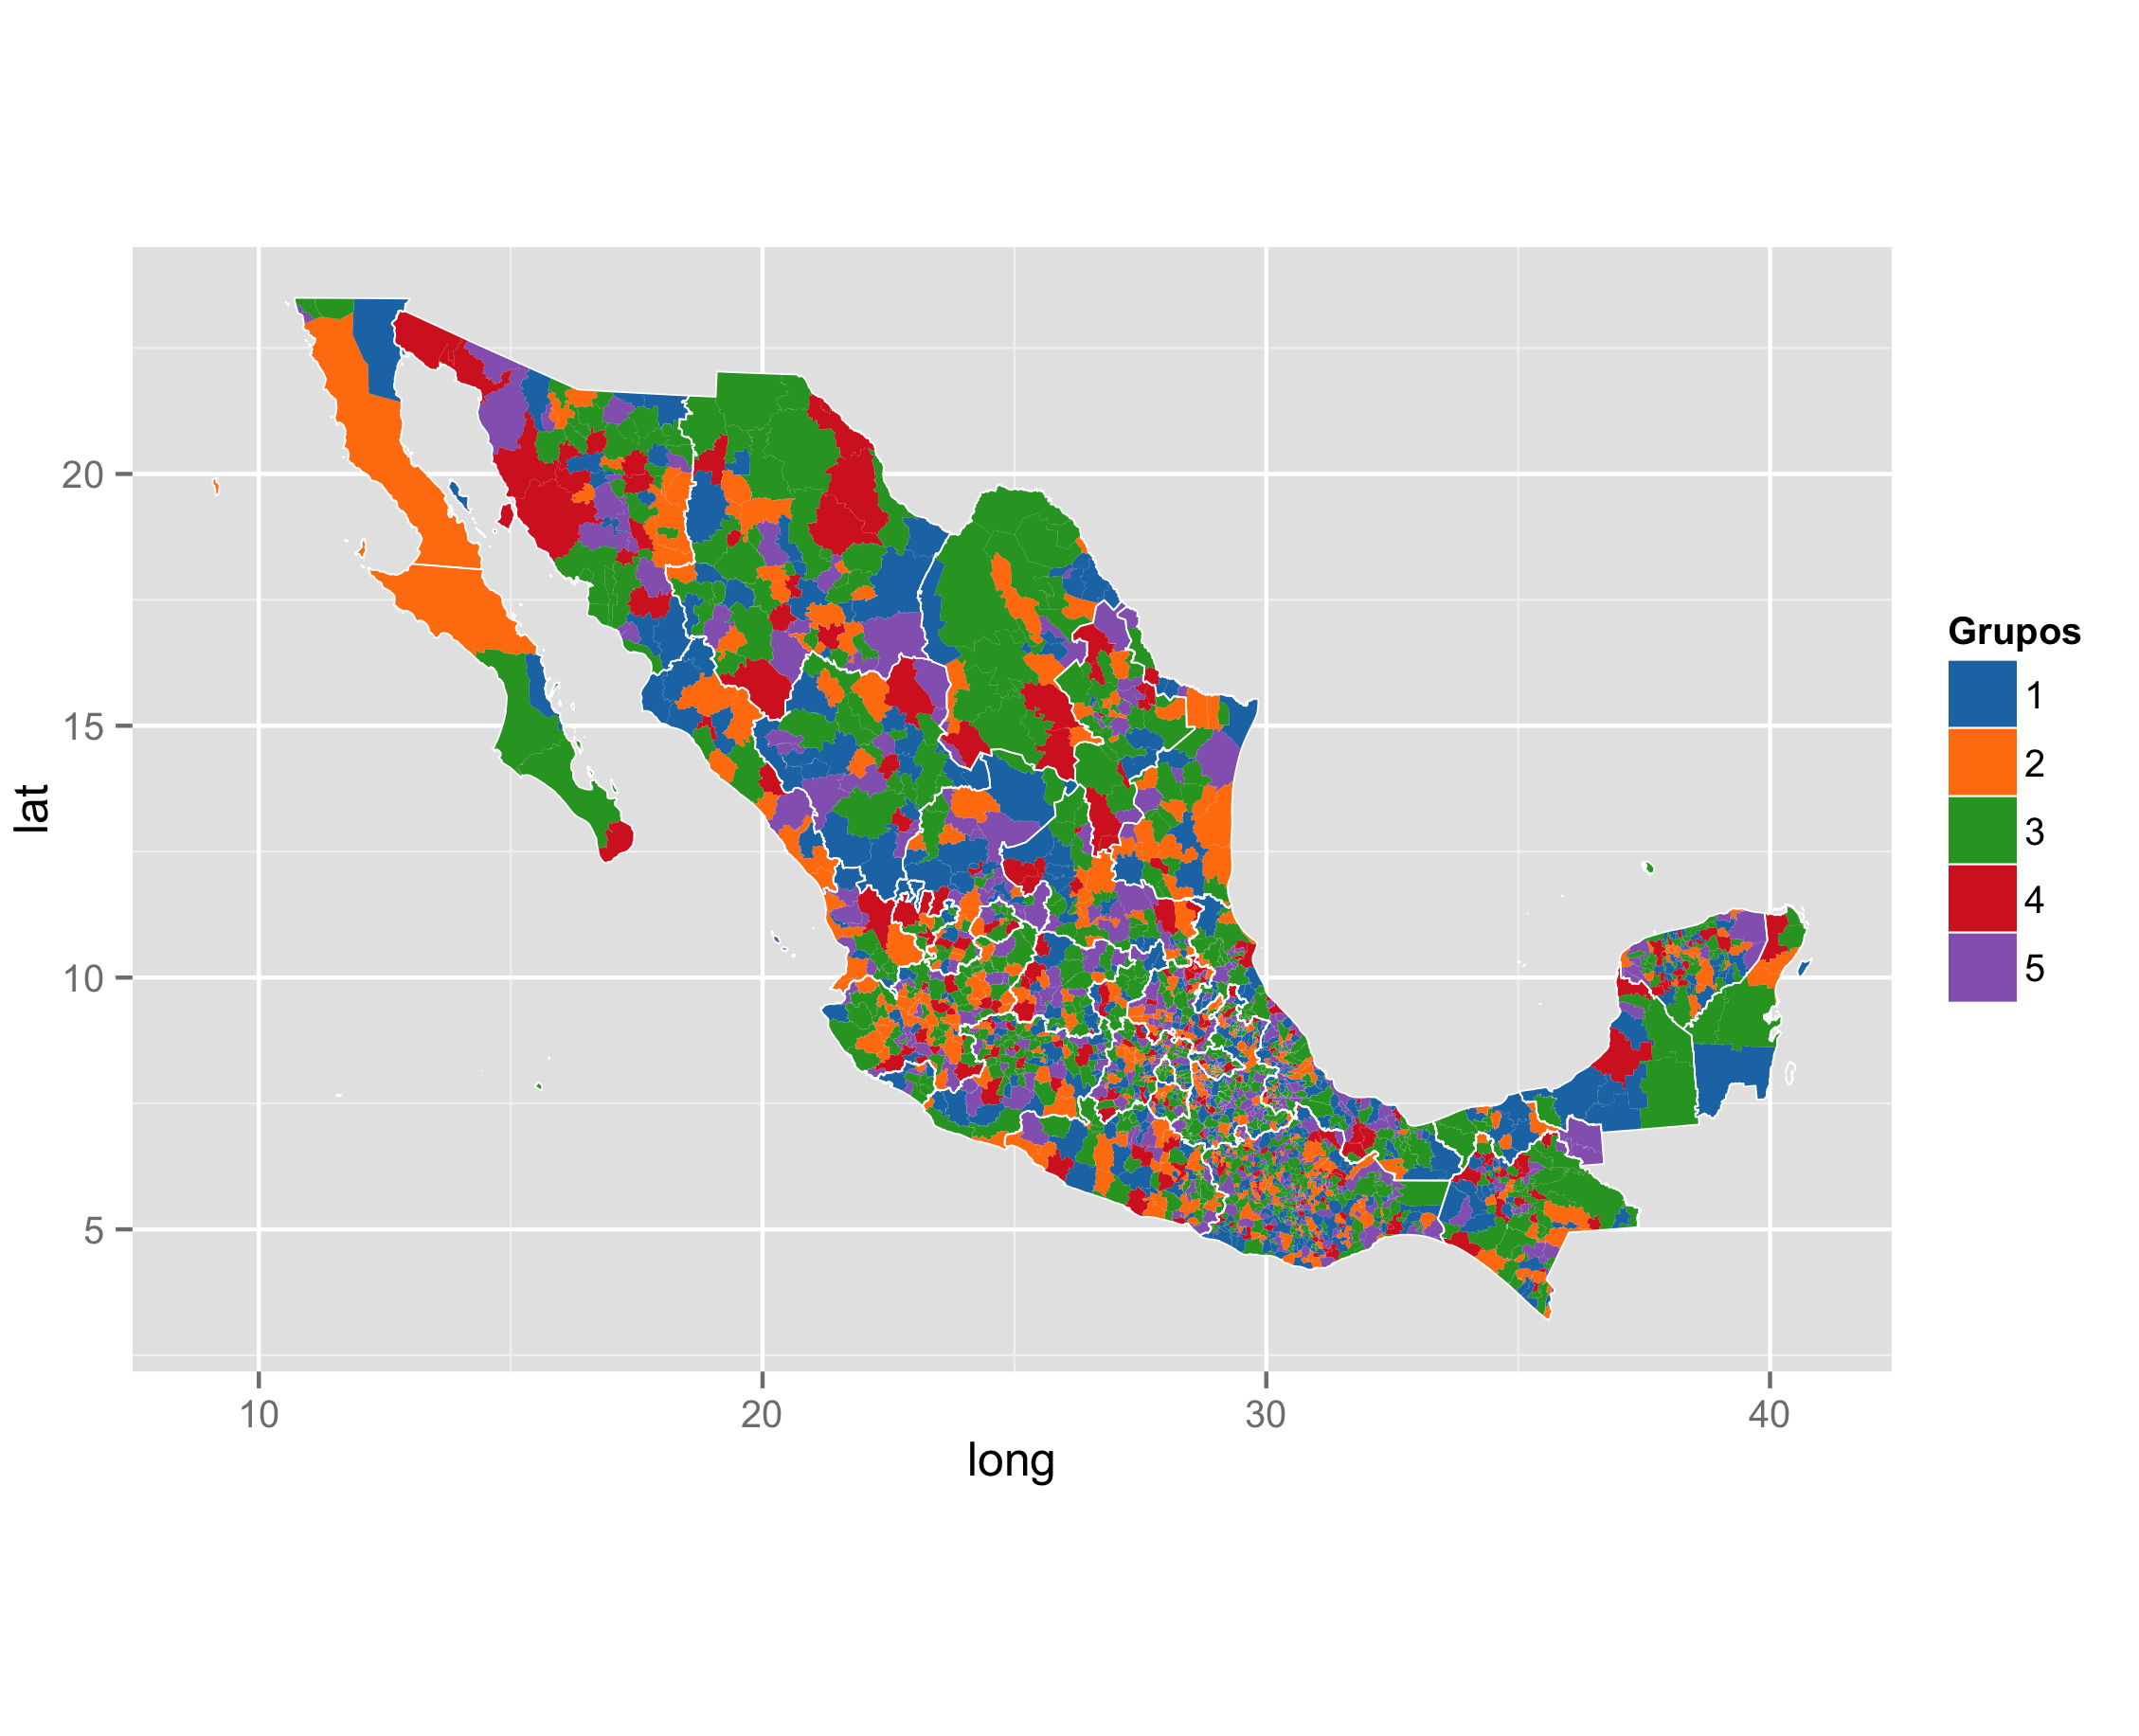
\includegraphics[width=\textwidth]{./maps/rmap5g.png} \\
  \caption{ Permutación aleatoria de los grupos obtenidos mediante el algoritmo de $k$-medias esféricas.}
  \label{fig:rmap_5g_ej}  
\end{figure}
Ahora, corroboramos lo dicho haciendo pruebas de hipótesis sobre $N_{rr}$ , $r=1, 2, 3, 4, 5$.

\subsubsection{Bajo supuesto de normalidad}
Suponiendo que $N_{11}, N_{22}, \dots, N_{55}$ se distribuyen normal, la tabla \ref{tab:conteobordesprueba} muestra la misma información que la tabla \ref{tab:conteobordes} para conteo de bordes del mismo tipo, pero se añade el valor $p$ porque ya estamos suponiendo una distribución.

\begin{table}[ht]
\centering
\begin{tabular}{rrrrrr}
  \hline
  grupo & $\Hat{N_{rs}}$  & $N_{rs,0}$ & $\Var$ & $z$ & valor-p \\ 
  \hline
  1 & 98.61 & 48.80 & 6.53 & 19.49 & $< 2.2 \times 10^{-16}$ \\ 
  2 & 110.35 & 42.07 & 5.77  & 28.43 & $< 2.2 \times 10^{-16}$ \\ 
  3 & 194.99 & 132.80 & 14.00 & 16.62 & $< 2.2 \times 10^{-16}$ \\ 
  4 & 50.36 & 15.23 & 2.36 & 22.88 & $< 2.2 \times 10^{-16}$ \\ 
  5 & 63.59 & 37.40 & 5.22 & 11.46 & $< 2.2 \times 10^{-16}$ \\ 
   \hline
\end{tabular}
\caption{Pruebas de hipótesis para $N_{rr}$ , $r=1, 2, 3, 4, 5$.}
\label{tab:conteobordesprueba}
\end{table}

Ahora, interpretando el valor $z$ bajo el supuesto de normalidad, los conteos $\Hat{N_{rs}}$'s caen muy lejos de la región de no rechazo. Por lo tanto, rechazamos la hipótesis nula de no autocorrelación espacial.


\subsubsection{Simulaciones de Monte Carlo}
Ahora, realizamos la prueba omitiendo el supuesto de normalidad. Sean $N_{rs,0}^*$ y $\Var^*$ el valor esperado y la varianza esperada, ambos calculados a partir de la muestra de Monte Carlo. Usando una muestra de tamaño $n_{sim}=9999$, podemos ver los resultados en la tabla \ref{tab:joincountsmontecarlo}.

% latex table generated in R 3.0.2 by xtable 1.7-3 package
% Thu Oct 30 11:32:06 2014
\begin{table}[!ht]
\centering
\begin{tabular}{rrrrrr}
  \hline
 grupo & $\Hat{N_{rs}}$  & $N_{rs,0}^*$ & $\Var^*$ & orden & valor-p \\ 
  \hline
  1 & 98.61 & 48.82 & 6.44 & 10000 & $1\times 10^{-4}$ \\ 
  2 & 110.35 & 42.11 & 5.92 & 10000 & $1\times 10^{-4}$ \\ 
  3 & 194.99 & 132.86 & 13.68 & 10000 & $1\times 10^{-4}$ \\ 
  4 & 50.36 & 15.23 & 2.34 & 10000 & $1\times 10^{-4}$ \\ 
  5 & 63.59 & 37.37 & 5.26 & 10000 & $1\times 10^{-4}$ \\ 
   \hline
\end{tabular}
\caption{Resultados de simulaciones de Monte Carlo.}
\label{tab:joincountsmontecarlo}
\end{table}

El conteo $\Hat{N_{rr}}$ es mayor que las $9,999$ simulaciones de Monte Carlo , para $r=1,2,3,4,5$. Es decir, para todos los grupos, se rechaza la hipótesis nula de no autocorrelación. Podemos ver la distribución de las muestras simuladas y donde caen los valores observados en la gráfica \ref{obj:jcdensity}.

\begin{figure}[!ht]
  \centering
  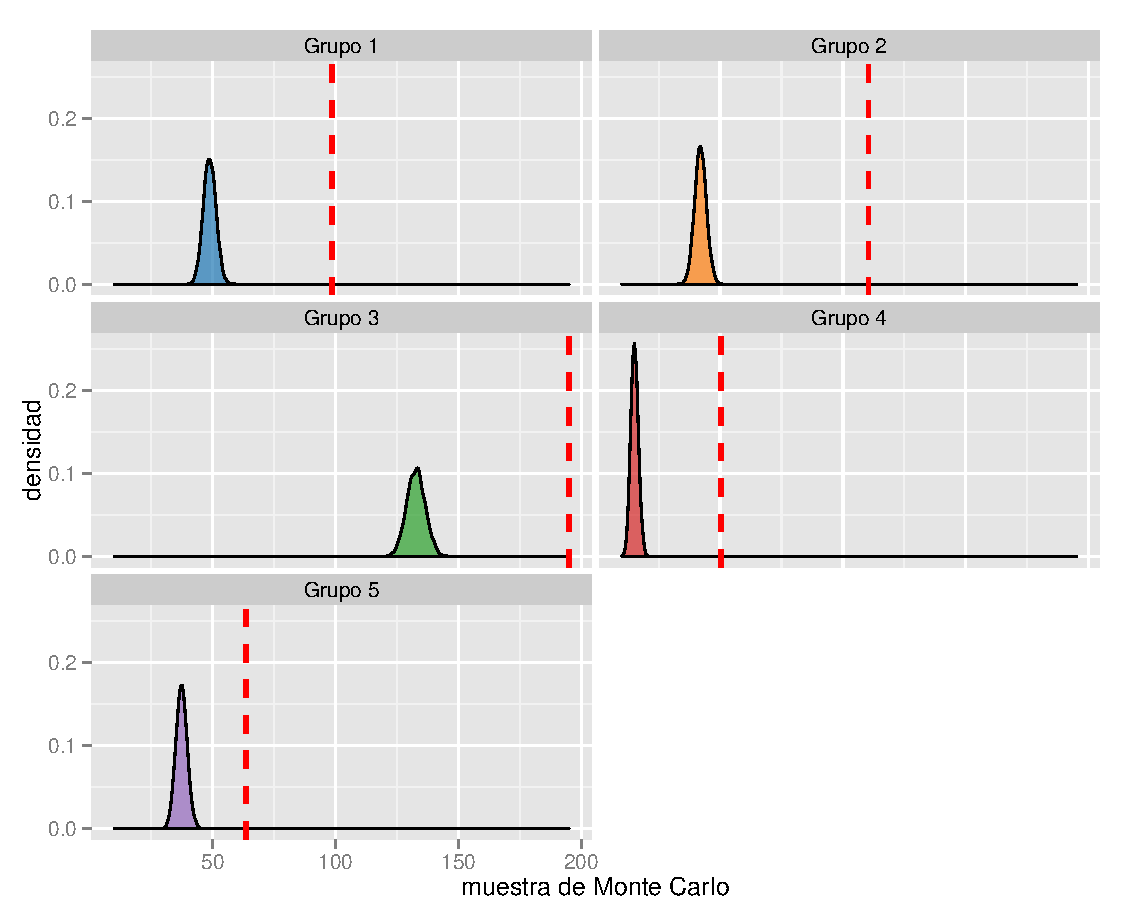
\includegraphics[width=\textwidth]{./plots/jc_density.pdf}
  \caption{Densidad de la muestra de Monte Carlo de $N_{rr}$. La línea punteada índica donde se encuentra $\Hat{N_{rr}}$. \label{obj:jcdensity} }
\end{figure}

\chapter{Conclusiones}
Después de haber realizado el análisis de conglomerados y las pruebas de autocorrelación espacial, se obtuvieron los siguientes resultados:

\begin{itemize}

\item Las pruebas sobre los índices $\mathcal{I}$ y $\mathcal{C}$ mostraron alta autocorrelación espacial positiva en el índice de marginación. Cómo se observó en el mapa \ref{obj:mapmarg} hay aglomeraciones muy marcadas. Las zonas más marginadas corresponden principalmente a municipios con población indígena y de difícil acceso.

\item A partir del análisis de conglomerados esférico sobre las variables de marginación, se encontró una estructura espacial latente entre los municipios:

\begin{itemize}
\item Dentro del análisis de conglomerados, el estadístico Gap mostró que 5 es un número óptimo de grupos y se utilizó el algoritmo de $k$-medias esféricas para hacer los conglomerados. En el primer grupo cayeron municipios con localidades de pocos habitantes y con grado marginación de media a bajo; en el segundo, cayeron los municipios más marginados cuyo principal rasgo es la carencia de agua entubada; el tercer grupo tiene municipios con grado de marginación de medio a alto, lo que lo separa del grupo dos es que tiene mayor porcentaje de viviendas con agua entubada; en el cuarto, se agruparon los municipios con menor grado de marginación; y en el quinto, cayeron municipios con características similares al del primer grupo pero se diferencia en que cuenta con localidades más grandes.

\item Para comprobar la autocorrelación espacial positiva de los grupos obtenidos, se utilizaron los estadísticos $N_{ss}$ de conteo de fronteras. Los conteos entre fronteras del mismo grupo son significativamente mayores a los conteos esperados, indicando un grado de asociación espacial alto.
\end{itemize}
\end{itemize}

La importancia de este estudio está en que nos permite identificar aglomeraciones en el mapa y conocer las necesidades de éstas. Esto permite definir estrategias en materia de infraestructura para poder atender las carencias o necesidades de cada uno de los municipios. Por ejemplo, la instalación de centros de salud o de atención en una zona céntrica en la Sierra Tarahumara. 

Es importante señalar que la marginación de un municipio podría estar correlacionada con otras variables, como la dificultad de acceso o las condiciones geográficas del municipio.

\section*{Otros enfoques posibles}
\begin{itemize}
\item Podría realizarse un análisis similar para identificar focos rojos de violencia, necesidades en cuestión de salud e incluso para identificar segmentos de mercado por región.
\item Si quisiéramos hacer un estudio más puntual, podríamos realizar el mismo estudio a nivel AGEB (Área Geoestadística Básica) o por manzana, enfocándonos en una región específica.
\item También es posible realizar estudios espacio-temporales para ver la evolución de la marginación de los municipios a través del tiempo.
\end{itemize}









\appendix
\chapter{Software y Reproducibilidad}
Se puede encontrar una copia de este trabajo en el siguiente URL: \href{https://github.com/carlosespino11/tesis}{https://github.com/carlosespino11/tesis}. 

Ahí se encuentran todos los datos y archivos necesarios para generar todas las figuras, el documento escrito y el código para replicar todos los resultados de este trabajo.

Software utilizado:
\begin{itemize}
\item R
\item \LaTeX
\end{itemize}
{
\nocite{*}
\ssp
\def\newblock{}
\bibliographystyle{myplainnat}
\bibliography{biblio}

}

\end{document}
